% Complex Tori and Elliptic Curves -- textbook expansion of
% ../torus_elliptic_group_law_notes.tex.  See PLAN.md for the full outline.
%
% Build (run from inside book/ so \sagedir = ../sagemath resolves):
%     cd book && pdflatex main.tex && pdflatex main.tex
% Re-run sagemath/build_coords.sh first if any Sage figure script changed.

\documentclass[11pt]{book}

\usepackage[margin=1in]{geometry}
\usepackage{amsmath,amssymb,amsthm,mathtools}
\usepackage{enumitem}
\usepackage{hyperref}
\usepackage{tikz}
\usetikzlibrary{arrows.meta,calc,positioning,decorations.markings,decorations.pathmorphing,
  patterns,shadings,shapes.geometric,fadings,backgrounds,intersections,bending}

\definecolor{formteal}{HTML}{1f4e79}
\definecolor{formgold}{HTML}{b88a14}
\definecolor{formrust}{HTML}{a8431d}
\definecolor{formplum}{HTML}{6b2e6e}
\definecolor{formsage}{HTML}{467b3a}
\definecolor{formslate}{HTML}{3a5168}
\definecolor{formivory}{HTML}{f6efe0}

% Location of the Sage-generated coordinate files, relative to the directory
% pdflatex is run from. Compile the book from inside book/:
%     cd book && pdflatex main.tex
% If you compile from elsewhere, redefine \sagedir to point at ../sagemath.
\newcommand{\sagedir}{../sagemath}

% Sage-computed precise coordinates for every TikZ figure.
% Generated by sagemath/build_coords.sh.
\input{\sagedir/coords.tex}

% Precise torus rendering computed by sagemath/08_torus_render.sage.
% Includes the outer and inner silhouettes plus six meridians and four
% latitude circles, each split into visible/hidden arcs.
\input{\sagedir/coords_torus.tex}

% Precise elliptic curve y^2 = 4x^3 - 4x sample points.
% Computed by sagemath/12_curve_sample.sage.
% Provides \curveOvalFull (smooth-cycle), \curveOvalUpper, \curveOvalLower,
% \curveBranchUpper, \curveBranchLower (all clipped at y = \curveYclip).
\input{\sagedir/coords_curve_sample.tex}

% Convenience macro that paints the precise torus inside the current scope.
% Usage:  \begin{scope}[shift={(...)}, scale=...] \drawprecisetorus \end{scope}
% The sage script computes for tilt angle beta = 60 deg:
%   - outer silhouette  (\torusOuter, closed curve)
%   - inner silhouette  (\torusInner, closed curve = donut-hole outline)
%   - 8 meridians at v = k pi/4 (small circles), split into visible/hidden arcs
%   - 4 longitudes at u in {0, pi/2, pi, 3pi/2} (latitude circles),
%     split into visible/hidden arcs
\newcommand{\drawprecisetorus}{%
  % (1) Fill the visible torus body with light teal.
  \fill[formteal!13, line join=round]
    plot[smooth cycle] coordinates {\torusOuter};
  % (2) Cut out the donut hole using the inner silhouette curve.
  \fill[white, line join=round]
    plot[smooth cycle] coordinates {\torusInner};
  % (3) Visible meridian arcs (eight small circles spaced 45 deg apart).
  % Back meridians (v in [0, pi]) form one visible arc each;
  % front meridians (v in (pi, 2 pi)) wrap across u = 0 and are split
  % into two visible chunks (VA and VB) by the sampling boundary.
  \draw[draw=formteal!60!black, line width=0.42pt, line join=round, opacity=0.9]
    plot[smooth] coordinates {\torusMerZeroVA};
  \draw[draw=formteal!60!black, line width=0.42pt, line join=round, opacity=0.9]
    plot[smooth] coordinates {\torusMerOneVA};
  \draw[draw=formteal!60!black, line width=0.42pt, line join=round, opacity=0.9]
    plot[smooth] coordinates {\torusMerTwoVA};
  \draw[draw=formteal!60!black, line width=0.42pt, line join=round, opacity=0.9]
    plot[smooth] coordinates {\torusMerThreeVA};
  \draw[draw=formteal!60!black, line width=0.42pt, line join=round, opacity=0.9]
    plot[smooth] coordinates {\torusMerFourVA};
  \draw[draw=formteal!60!black, line width=0.42pt, line join=round, opacity=0.9]
    plot[smooth] coordinates {\torusMerFiveVA};
  \draw[draw=formteal!60!black, line width=0.42pt, line join=round, opacity=0.9]
    plot[smooth] coordinates {\torusMerFiveVB};
  \draw[draw=formteal!60!black, line width=0.42pt, line join=round, opacity=0.9]
    plot[smooth] coordinates {\torusMerSixVA};
  \draw[draw=formteal!60!black, line width=0.42pt, line join=round, opacity=0.9]
    plot[smooth] coordinates {\torusMerSixVB};
  \draw[draw=formteal!60!black, line width=0.42pt, line join=round, opacity=0.9]
    plot[smooth] coordinates {\torusMerSevenVA};
  \draw[draw=formteal!60!black, line width=0.42pt, line join=round, opacity=0.9]
    plot[smooth] coordinates {\torusMerSevenVB};
  % (4) Visible longitude arcs (the four canonical latitude circles).
  % Outer (u=0) is visible only on the front half (v in (pi, 2 pi)),
  % inner (u=pi) only on the back half (v in (0, pi)); the top crest
  % (u=pi/2) is visible everywhere; the bottom (u=3pi/2) is fully hidden.
  \draw[draw=formteal!60!black, line width=0.5pt, line join=round, opacity=0.95]
    plot[smooth] coordinates {\torusLonTopVA};
  \draw[draw=formteal!60!black, line width=0.42pt, line join=round, opacity=0.8]
    plot[smooth] coordinates {\torusLonOuterVA};
  \draw[draw=formteal!60!black, line width=0.42pt, line join=round, opacity=0.8]
    plot[smooth] coordinates {\torusLonInnerVA};
  % (5) Crisp silhouette outlines drawn last so they sit on top.
  \draw[draw=formteal!65!black, line width=0.95pt, line join=round]
    plot[smooth cycle] coordinates {\torusOuter};
  \draw[draw=formteal!65!black, line width=0.8pt, line join=round]
    plot[smooth cycle] coordinates {\torusInner};
}

% Precise sphere (CP^1) rendering, matching the torus style.
% Computed by sagemath/10_sphere_render.sage at gamma = 30 deg elevation.
% Provides:
%   \sphereOutline    -- silhouette as a closed coordinate list (unit circle)
%   \sphereLatXY{V,H}A -- equator/tropics/etc. visible/hidden arcs
%   \sphereMerXyz{V,H}A -- eight meridians at v = k*pi/4
%   \sphereNorth{x,y}, \sphereSouth{x,y} -- pole projection coordinates
\newcommand{\drawprecisesphere}{%
  % Color tone matches the torus (formteal) for visual unity across figures.
  % (1) Flat-filled body of the sphere (same filling style as the torus)
  \fill[formteal!13, line join=round]
    plot[smooth cycle] coordinates {\sphereOutline};
  % (2) Visible latitude arcs
  \draw[draw=formteal!60!black, line width=0.45pt, line join=round, opacity=0.9]
    plot[smooth] coordinates {\sphereLatEquatorVA};
  \draw[draw=formteal!60!black, line width=0.4pt, line join=round, opacity=0.85]
    plot[smooth] coordinates {\sphereLatNorthVA};
  \draw[draw=formteal!60!black, line width=0.4pt, line join=round, opacity=0.85]
    plot[smooth] coordinates {\sphereLatNorthVB};
  \draw[draw=formteal!60!black, line width=0.4pt, line join=round, opacity=0.85]
    plot[smooth] coordinates {\sphereLatTropicVA};
  \draw[draw=formteal!60!black, line width=0.4pt, line join=round, opacity=0.85]
    plot[smooth] coordinates {\sphereLatTropicVB};
  \draw[draw=formteal!60!black, line width=0.4pt, line join=round, opacity=0.85]
    plot[smooth] coordinates {\sphereLatSouthVA};
  % (3) Visible meridian arcs (eight meridians at v = k pi/4)
  \draw[draw=formteal!60!black, line width=0.42pt, line join=round, opacity=0.9]
    plot[smooth] coordinates {\sphereMerZeroVA};
  \draw[draw=formteal!60!black, line width=0.42pt, line join=round, opacity=0.9]
    plot[smooth] coordinates {\sphereMerOneVA};
  \draw[draw=formteal!60!black, line width=0.42pt, line join=round, opacity=0.9]
    plot[smooth] coordinates {\sphereMerTwoVA};
  \draw[draw=formteal!60!black, line width=0.42pt, line join=round, opacity=0.9]
    plot[smooth] coordinates {\sphereMerThreeVA};
  \draw[draw=formteal!60!black, line width=0.42pt, line join=round, opacity=0.9]
    plot[smooth] coordinates {\sphereMerFourVA};
  \draw[draw=formteal!60!black, line width=0.42pt, line join=round, opacity=0.9]
    plot[smooth] coordinates {\sphereMerFiveVA};
  \draw[draw=formteal!60!black, line width=0.42pt, line join=round, opacity=0.9]
    plot[smooth] coordinates {\sphereMerSixVA};
  \draw[draw=formteal!60!black, line width=0.42pt, line join=round, opacity=0.9]
    plot[smooth] coordinates {\sphereMerSevenVA};
  % (4) Hidden back arcs as dashed light strokes
  \draw[draw=formteal!50!black, dashed, line width=0.3pt, line join=round, opacity=0.55]
    plot[smooth] coordinates {\sphereLatEquatorHA};
  % (5) Crisp silhouette outline on top
  \draw[draw=formteal!65!black, line width=0.95pt, line join=round]
    plot[smooth cycle] coordinates {\sphereOutline};
}

% Convenience macro that draws the real locus of E: y^2 = 4x^3 - 4x
% using pre-computed coordinate lists from sagemath/12_curve_sample.sage.
% Usage:  \begin{scope}[shift={(...)}, scale=...] \drawprecisecurve \end{scope}
% The scope should set up an appropriate coordinate system.
% This macro draws only the curve arcs and branch-point dots; the caller
% is responsible for axes and labels.
\newcommand{\drawprecisecurve}{%
  % Oval (compact component, x in [-1,0]): draw as closed smooth cycle.
  \draw[draw=formteal!60!black, line width=0.88pt, line join=round]
    plot[smooth cycle, tension=0.85] coordinates {\curveOvalFull};
  % Branch (unbounded component, x >= 1): upper and lower arcs.
  \draw[draw=formteal!60!black, line width=0.88pt, line join=round]
    plot[smooth, tension=0.9] coordinates {\curveBranchUpper};
  \draw[draw=formteal!60!black, line width=0.88pt, line join=round]
    plot[smooth, tension=0.9] coordinates {\curveBranchLower};
  % Branch points (Weierstrass roots e1=-1, e2=0, e3=1)
  \fill[formteal!70!black] (-1,0) circle (1.8pt);
  \fill[formteal!70!black] ( 0,0) circle (1.8pt);
  \fill[formteal!70!black] ( 1,0) circle (1.8pt);
}

\setlist[enumerate]{leftmargin=*, itemsep=0.35em}
\setlist[itemize]{leftmargin=*, itemsep=0.25em}
\allowdisplaybreaks
\emergencystretch=2em

\newcommand{\C}{\mathbb{C}}
\newcommand{\R}{\mathbb{R}}
\newcommand{\Z}{\mathbb{Z}}
\newcommand{\Q}{\mathbb{Q}}
\newcommand{\F}{\mathbb{F}}
\newcommand{\CP}{\mathbb{CP}}
\newcommand{\HH}{\mathbb{H}}
\newcommand{\OO}{\mathcal{O}}
\newcommand{\M}{\mathcal{M}}
\newcommand{\Div}{\operatorname{Div}}
\newcommand{\Pic}{\operatorname{Pic}}
\newcommand{\Prin}{\operatorname{Prin}}
\newcommand{\Jac}{\operatorname{Jac}}
\newcommand{\smap}{\mathfrak{s}}% Abel--Jacobi sum map Div^0(T) -> T (distinct from Weierstrass sigma)
\newcommand{\Span}{\operatorname{span}}
\newcommand{\divisor}{\operatorname{div}}
\newcommand{\ord}{\operatorname{ord}}
\newcommand{\id}{\operatorname{id}}
\newcommand{\Res}{\operatorname{Res}}
\newcommand{\degdiv}{\operatorname{deg}}
\newcommand{\dd}{\,d}
\newcommand{\wpprime}{\wp'}
\newcommand{\LambdaLat}{\Lambda}

% Textbook theorem environments: all share a single counter that resets each
% chapter (Theorem 2.1, Proposition 2.2, Definition 2.3, ...) so statements read
% in one sequence. thmtools' `sibling=theorem' gives the shared numbering, while
% each environment keeps its OWN label type, so cleveref prints the right word
% (\cref to a Proposition reads "proposition 2.2", not "theorem 2.2").
% Environment NAMES match the source notes, so reused content drops in unchanged.
\usepackage{thmtools}
\declaretheorem[name=Theorem,numberwithin=chapter]{theorem}
\declaretheorem[name=Proposition,sibling=theorem]{proposition}
\declaretheorem[name=Lemma,sibling=theorem]{lemma}
\declaretheorem[name=Corollary,sibling=theorem]{corollary}
\declaretheorem[name=Definition,sibling=theorem,style=definition]{definition}
\declaretheorem[name=Example,sibling=theorem,style=definition]{example}
\declaretheorem[name=Remark,sibling=theorem,style=remark]{remark}
% `warning' cannot use that environment name directly inside thmtools, because
% the internal \@warning is already reserved (by amsmath/mathtools). We declare
% it under the safe name `warningthm' (sibling => shared theorem counter, so it
% joins the Theorem/Proposition/... sequence) and alias \warning to it, so
% authors still write \begin{warning} ... \end{warning}.
\declaretheorem[name=Warning,sibling=theorem,style=remark]{warningthm}
\let\warning\warningthm
\let\endwarning\endwarningthm
% Exercises run on their own per-chapter counter.
\declaretheorem[name=Exercise,numberwithin=chapter,style=definition]{exercise}

\newenvironment{keyidea}[1]{%
  \par\medskip
  \begin{center}
  \begin{minipage}{0.92\textwidth}
  \hrule
  \smallskip
  \textbf{#1.}\quad\ignorespaces
}{%
  \smallskip
  \hrule
  \end{minipage}
  \end{center}
  \medskip
}

\tikzset{
  arrow/.style={-{Latex[length=2mm]}, thick},
  point/.style={circle, fill=black, inner sep=1.5pt},
  labelnode/.style={font=\small, align=center},
  note/.style={draw=black!55, rounded corners=2pt, align=center, inner sep=5pt, fill=black!3},
  visualnode/.style={draw=black!60, rounded corners=2pt, align=center, inner sep=6pt, fill=black!2}
}

% Smart cross-references (\cref / \Cref). Load last, after hyperref.
\usepackage{cleveref}
% cleveref has built-in names for theorem/proposition/lemma/corollary/
% definition/remark/example, so those resolve automatically. The two custom
% types -- `warning' and `exercise' -- have no built-in, so name them here.
% Lowercase singular is for \cref ("exercise 2.3"); capitalized for \Cref.
\crefname{warningthm}{warning}{warnings}
\Crefname{warningthm}{Warning}{Warnings}
\crefname{exercise}{exercise}{exercises}
\Crefname{exercise}{Exercise}{Exercises}


\title{Complex Tori and Elliptic Curves\\
\large Why the Abelian Group Law Must Be the Chord--Tangent Law\\
via the $\wp$-Embedding}
\author{}
\date{Spring 2026}

\begin{document}

\frontmatter
\maketitle

\begin{center}
\emph{A textbook developed from midterm and final exam themes:
differential forms, residues, compact Riemann surfaces, divisors,
Riemann--Roch, complex tori, and the Weierstrass $\wp$-function.}
\end{center}

\chapter*{Preface}
\addcontentsline{toc}{chapter}{Preface}

This book explains one fact in full: the chord--tangent law on a smooth plane
cubic is not an arbitrary geometric trick but the abelian group law on the complex
torus $\C/\Lambda$, carried onto the cubic by the Weierstrass functions $\wp$ and
$\wp'$. Addition on the torus is addition of complex numbers modulo a lattice ---
associative and commutative for the most elementary reasons --- and the embedding
$z \mapsto [\wp(z):\wp'(z):1]$ turns it into ``draw a line, take the third
intersection, reflect.'' Seen this way, every feature of the chord--tangent rule,
including the puzzling reflection step, is forced.

The treatment is meant to be \emph{self-contained}. The genus-one theory is built
from a single course in complex analysis: the dimension counts that single out
$1, \wp, \wp'$ are derived elementarily from Liouville's theorems and the explicit
Weierstrass functions, and the converse of Abel's law is proved constructively
with the Weierstrass $\sigma$-function. Riemann--Roch is stated as the general
theorem for context, but nothing in the book depends on it. Every figure is drawn
from coordinates computed exactly by the Sage scripts of \cref{app:C}, so the
pictures are reproducible rather than schematic, and roughly eighty exercises, all
with complete solutions in \cref{app:D}, let the reader reconstruct the theory.

\paragraph{Audience and prerequisites.}
The intended reader is a strong final-year undergraduate or beginning graduate
student. We assume one course in single-variable complex analysis (holomorphic and
meromorphic functions, Laurent series, residues, Liouville's theorem, the argument
principle --- all recalled in \cref{app:A}), comfort with quotient spaces, and the
rudiments of abelian groups and linear algebra. No prior acquaintance with Riemann
surfaces, divisors, or Riemann--Roch is needed.

\paragraph{How to read it.}
The chapters are linear, and \cref{fig:dependency} maps the whole argument on the
first pages. A reader meeting the subject for the first time may skim the
convergence, Eisenstein-series, and field-generation material of
\cref{ch:weierstrass_wp} --- the most technical in the book --- without losing the
main thread. The List of Symbols that follows fixes notation, and \cref{app:B}
records how the material grew out of a course's midterm and final.

\tableofcontents

\chapter*{List of Symbols}
\addcontentsline{toc}{chapter}{List of Symbols}

\begin{center}
\footnotesize
\begin{tabular}{@{}ll@{}}
\multicolumn{2}{@{}l}{\itshape Number systems and spaces}\\
\(\C, \R, \Z, \Q\) & complex, real, integer, rational numbers\\
\(\F\) & a field (e.g.\ a finite field \(\F_p\))\\
\(\CP^n\) & complex projective space\\
\(\HH\) & upper half-plane \(\{\operatorname{Im}\tau>0\}\)\\[2pt]
\multicolumn{2}{@{}l}{\itshape Lattices and the torus}\\
\(\Lambda = \Z\omega_1+\Z\omega_2\) & a lattice; \(\omega_1,\omega_2\) its periods\\
\(\tau = \omega_2/\omega_1\) & period ratio, normalized to \(\HH\)\\
\(P_\Lambda\) & fundamental parallelogram\\
\(T = \C/\Lambda\) & the complex torus\\
\(O\) & identity; image of \(0\); point at infinity of \(E\)\\
\(m(\Lambda)\) & least length of a nonzero lattice vector\\[2pt]
\multicolumn{2}{@{}l}{\itshape Weierstrass functions}\\
\(\wp,\ \wp'\) & Weierstrass function (double pole) and derivative\\
\(\zeta = \sigma'/\sigma\) & Weierstrass zeta function, \(\zeta' = -\wp\)\\
\(\sigma\) & Weierstrass sigma function\\
\(G_k\) & Eisenstein series of weight \(k\)\\
\(g_2, g_3\) & invariants, \(g_2 = 60G_4\), \(g_3 = 140G_6\)\\
\(\Delta\) & discriminant \(g_2^3 - 27g_3^2\)\\
\(e_1, e_2, e_3\) & roots of \(4x^3-g_2x-g_3\); values \(\wp(\omega_i/2)\)\\
\(\eta_k\) & quasi-periods, \(\eta_k = 2\zeta(\omega_k/2)\)\\
\(j\) & the \(j\)-invariant \(1728\,g_2^3/\Delta\)\\[2pt]
\multicolumn{2}{@{}l}{\itshape Functions and fields}\\
\(\OO,\ \M\) & holomorphic, meromorphic functions\\
\(\C(\wp,\wp')\) & field of elliptic functions\\[2pt]
\multicolumn{2}{@{}l}{\itshape Divisors and Riemann--Roch}\\
\(\Div(X),\ \Div^0(X)\) & divisors; degree-zero divisors\\
\(\divisor(f)\) & divisor of \(f\) (a principal divisor)\\
\(\ord_p,\ \Res,\ \degdiv\) & order at \(p\), residue, degree\\
\(\Prin(X)\) & principal divisors\\
\(\Pic(X),\ \Pic^0(X)\) & Picard group; degree-zero Picard group\\
\(K\) & canonical divisor (\(K\sim0\) on \(T\))\\
\(L(D),\ \ell(D)\) & Riemann--Roch space and its dimension\\
\(\smap,\ \bar\smap\) & Abel--Jacobi sum map \(\Div^0(T)\!\to\!T\) and \(\Pic^0(T)\!\to\!T\)\\[2pt]
\multicolumn{2}{@{}l}{\itshape The cubic and its group law}\\
\(E\) & the cubic \(Y^2Z = 4X^3 - g_2XZ^2 - g_3Z^3\)\\
\(\Phi\) & Weierstrass embedding \(T \to E\)\\
\(\oplus,\ \ominus\) & group law on \(E\) and its inverse (reflection)\\
\(\boxplus\) & chord--tangent operation (equal to \(\oplus\))\\
\end{tabular}
\end{center}

\mainmatter

\part{Tori as Riemann Surfaces}
% Introduction and Overview  (source §1; added: reading guide, dependency
% diagram as a labeled figure, main theorem stated up front)
\chapter{Introduction and Overview}
\label{ch:intro}

\section{A Construction That Should Not Work}
\label{sec:intro-construction}

Take a smooth cubic curve in the plane, for instance
\[
  E:\quad y^2 = 4x^3 - g_2 x - g_3,
\]
and the following recipe for ``adding'' two of its points. Given points
\(P\) and \(Q\) on \(E\), draw the straight line through them. A line meets a
cubic in three points, so it strikes \(E\) at one further point \(R\). Reflect
\(R\) across the \(x\)-axis to obtain a point we call \(P \oplus Q\). To add a
point to itself, use the tangent line at \(P\) in place of the chord. This is
the \emph{chord--tangent law}.

Nothing about this recipe looks like it should produce a group. Reflecting a
third intersection point is a geometric gesture, not an algebraic operation;
there is no visible reason for it to be associative, and no visible reason for
inverses to behave. Yet the chord--tangent law \emph{is} an abelian group law,
with associativity holding exactly. The standard elementary proofs of
associativity are long case analyses or invocations of the Cayley--Bacharach
theorem, and they leave the impression that the group structure is a lucky
accident of plane geometry.

It is not an accident. These notes explain the following single fact, which
makes every group axiom transparent at once.

\begin{quote}
The chord--tangent law on a smooth plane cubic is not an arbitrary geometric
trick. It is exactly the abelian group law on the complex torus
\(T = \C/\Lambda\), transported to the cubic by the Weierstrass functions
\(\wp\) and \(\wp'\).
\end{quote}

The slogan is
\[
  \boxed{
    \text{addition on } \C/\Lambda
    \quad\Longleftrightarrow\quad
    \text{chord--tangent addition on } E
  }
\]
where, in homogeneous coordinates \([X:Y:Z]\) on \(\CP^2\),
\[
  E:\quad Y^2 Z = 4X^3 - g_2 X Z^2 - g_3 Z^3 .
\]
On the torus side, addition is nothing more than addition of complex numbers
modulo a lattice \(\Lambda\); it is associative and commutative for the most
elementary of reasons. The entire mystery of the chord--tangent law dissolves
once we exhibit a dictionary between the two pictures.

\section{The Answer Stated First}
\label{sec:intro-answer}

We state the destination now, before any of the machinery is built, so that
every later chapter can be read as a step toward it. The terms appearing here
(\emph{lattice}, \emph{Weierstrass function}, \emph{divisor}, \emph{point at
infinity}) are defined from scratch in the chapters that follow; forward
references point to the precise statements.

\begin{theorem}[Main theorem]
\label{thm:main}
Let \(\Lambda \subset \C\) be a lattice and let \(\wp\) be the Weierstrass
function of \(\Lambda\), with derivative \(\wp'\). Set
\[
  E:\quad Y^2 Z = 4X^3 - g_2 X Z^2 - g_3 Z^3 \subset \CP^2 ,
\]
with \(g_2, g_3\) the invariants of \(\Lambda\). Then the map
\[
  \Phi : \C/\Lambda \longrightarrow E,
  \qquad
  \Phi(z) =
  \begin{cases}
    [\wp(z) : \wp'(z) : 1], & z \notin \Lambda,\\[2pt]
    [0 : 1 : 0] =: O,       & z \in \Lambda,
  \end{cases}
\]
is an isomorphism of compact Riemann surfaces, and it is an isomorphism of
groups when \(E\) carries the chord--tangent law and \(\C/\Lambda\) carries
addition modulo \(\Lambda\). Equivalently: three points of \(E\), counted with
intersection multiplicity, are collinear if and only if their \(\Phi\)-preimages
in \(\C/\Lambda\) sum to \(0\).
\end{theorem}

The map \(\Phi\) is constructed in \cref{ch:embedding}; that it lands on \(E\)
comes from the differential equation for \(\wp\) in \cref{ch:weierstrass_wp};
that it is a bijection of Riemann surfaces is \cref{ch:embedding}; and the
collinearity statement, which is the heart of the matter, is proved in
\cref{ch:lines_divisors,ch:transport} using Abel's sum law from
\cref{ch:abel}.

\begin{keyidea}{Main conclusion}
If a line meets the cubic in three points \(P, Q, R\), counted with
intersection multiplicity, then those three points add to zero in the group law
transported from the torus:
\[
  P + Q + R = O .
\]
Solving for \(P + Q\) gives
\[
  P + Q = -R .
\]
Geometrically, this means: draw the line through \(P\) and \(Q\), take the
third intersection \(R\), then reflect \(R\) across the \(x\)-axis.
\end{keyidea}

\section{The Chain of Ideas}
\label{sec:intro-chain}

The proof of \cref{thm:main} is a chain of structural facts, each of which is
of independent interest and each of which occupies one part of this book. The
logical skeleton is shown in \cref{fig:dependency}.

\begin{figure}[ht]
\centering
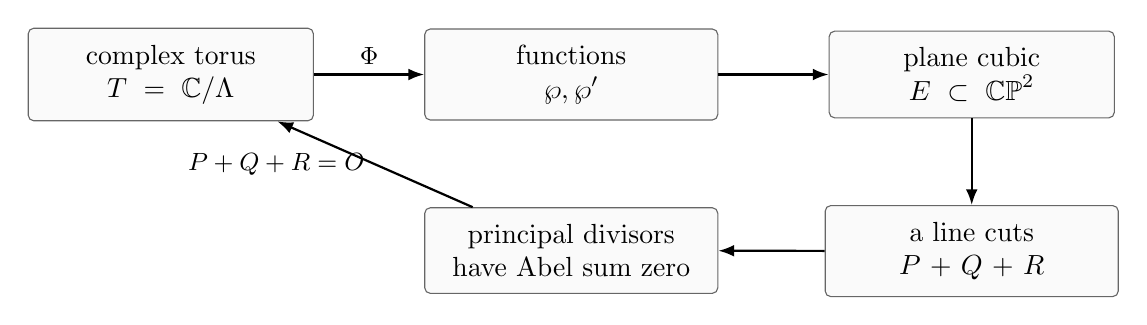
\begin{tikzpicture}[node distance=1.2cm]
  \node[visualnode, text width=3.2cm] (torus) {complex torus\\\(T=\C/\Lambda\)};
  \node[visualnode, text width=3.3cm, right=1.4cm of torus] (wp) {functions\\\(\wp,\wp'\)};
  \node[visualnode, text width=3.2cm, right=1.4cm of wp] (cubic) {plane cubic\\\(E\subset\CP^2\)};
  \node[visualnode, text width=3.3cm, below=1.1cm of wp] (div) {principal divisors\\have Abel sum zero};
  \node[visualnode, text width=3.3cm, below=1.1cm of cubic] (line) {a line cuts\\\(P+Q+R\)};
  \draw[arrow] (torus) -- node[above, labelnode] {\(\Phi\)} (wp);
  \draw[arrow] (wp) -- (cubic);
  \draw[arrow] (line) -- (div);
  \draw[arrow] (div) -- node[left, labelnode] {\(P+Q+R=O\)} (torus);
  \draw[arrow] (cubic) -- (line);
\end{tikzpicture}
\caption{The chain of ideas behind \cref{thm:main}. The torus supplies the
group law; the Weierstrass functions \(\wp,\wp'\) carry it onto the cubic
\(E\); a line meeting \(E\) in \(P,Q,R\) records the divisor \(P+Q+R\); that
divisor is principal, so by Abel's sum law its points sum to \(0\) back on the
torus. The loop closes, and the chord--tangent law is forced.}
\label{fig:dependency}
\end{figure}

Read clockwise from the upper left, the chain runs as follows.

\begin{enumerate}
\item \textbf{The torus carries an obvious group law.} The quotient
\(\C/\Lambda\) inherits addition from \(\C\). Associativity, commutativity, and
inverses are immediate because they already hold in \(\C\)
(\cref{ch:lattices,ch:torus_group_surface}).

\item \textbf{The torus is a Riemann surface of genus one.} As a smooth compact
surface \(\C/\Lambda \cong S^1 \times S^1\) is a doughnut; as a Riemann surface
it has genus one. This is what eventually forces the cubic equation
(\cref{ch:torus_group_surface}).

\item \textbf{Meromorphic functions on the torus are scarce.} A nonconstant
holomorphic function cannot exist (Liouville), and the orders of zeros and poles
of a meromorphic function obey rigid global constraints
(\cref{ch:elliptic_liouville,ch:divisors}).

\item \textbf{Riemann--Roch counts those functions.} On a genus-one surface the
dimension counts are sharp enough to single out a function with a double pole
(\(\wp\)) and one with a triple pole (\(\wp'\)), and to force a single algebraic
relation between them (\cref{ch:riemann_roch,ch:weierstrass_wp}).

\item \textbf{That relation is the cubic.} The differential equation
\(\wp'^2 = 4\wp^3 - g_2\wp - g_3\) says precisely that \((\wp,\wp')\) traces out
\(E\). The map \(\Phi\) of \cref{thm:main} is the resulting embedding
(\cref{ch:weierstrass_wp,ch:embedding}).

\item \textbf{Lines cut principal divisors.} A line meeting \(E\) at \(P,Q,R\)
defines a meromorphic function on \(E\) whose divisor is
\(P + Q + R - 3O\). Pulled back to the torus, principal divisors have Abel sum
zero, which is exactly \(P + Q + R = O\)
(\cref{ch:abel,ch:lines_divisors,ch:transport}).
\end{enumerate}

Everything after that --- the explicit chord and tangent formulas, the role of
the point at infinity as the identity, the two-torsion points, the closed-form
addition laws --- is the working-out of this one loop
(\crefrange{ch:chord_tangent_cases}{ch:synthesis}).

\section{How to Read This Book}
\label{sec:intro-reading}

The book is organized into six parts that follow the chain above.

\begin{description}[leftmargin=1.4em, style=nextline]
\item[Part I --- Tori as Riemann Surfaces
  (\cref{ch:lattices,ch:torus_group_surface}).]
  Lattices, the quotient \(\C/\Lambda\), its complex structure, its group law,
  and its genus.
\item[Part II --- Elliptic Functions
  (\cref{ch:elliptic_liouville,ch:divisors}).]
  Doubly periodic meromorphic functions, Liouville's theorems, orders, and
  divisors.
\item[Part III --- Riemann--Roch on Genus One (\cref{ch:riemann_roch}).]
  The spaces \(L(D)\), the canonical divisor, and the dimension counts that
  make \(\wp\) and \(\wp'\) inevitable.
\item[Part IV --- The Weierstrass Functions
  (\cref{ch:weierstrass_wp,ch:embedding}).]
  Construction of \(\wp\), the differential equation, and the embedding
  \(\Phi\) into \(\CP^2\). The convergence, Eisenstein-series, and
  field-generation material of \cref{ch:weierstrass_wp} is the most technical in
  the book (graduate level) and may be skimmed on a first reading without losing
  the main thread.
\item[Part V --- The Group Law on the Cubic
  (\crefrange{ch:abel}{ch:chord_tangent_cases}).]
  Abel's sum law, lines as principal divisors, the transport of the group law,
  and the chord--tangent law case by case.
\item[Part VI --- Formulas, Computations, and Synthesis
  (\crefrange{ch:coordinate_formulas}{ch:synthesis}).]
  Closed-form addition and doubling formulas, the analytic addition formula, a
  fully worked numerical example, and pointers onward.
\end{description}

Four appendices support the main text.
\Cref{app:A} is a self-contained refresher on the complex analysis the book
relies on (Liouville's theorem, residues, the argument principle, Laurent
series); a reader who is rusty should skim it first.
\Cref{app:B} records how the present material grew out of a course's midterm and
final examinations, for readers who want that bridge.
\Cref{app:C} documents the Sage scripts that compute the exact coordinates for
every figure, so that all pictures are reproducible.
\Cref{app:D} contains full solutions to every exercise.

\paragraph{Prerequisites.}
We assume one course in single-variable complex analysis (holomorphic and
meromorphic functions, Laurent series, residues, Liouville's theorem, the
argument principle), comfort with quotient spaces from point-set topology, and
the basics of abelian groups and linear algebra. No prior exposure to Riemann
surfaces, divisors, or Riemann--Roch is assumed; these are developed here in the
single case of genus one.

\paragraph{Standing notation.}
The following symbols are fixed throughout. The complex numbers, reals, and
integers are \(\C\), \(\R\), \(\Z\); the upper half-plane is \(\HH\); and
\(\CP^n\) is complex projective space. A \emph{lattice} is written
\(\Lambda = \Z\omega_1 + \Z\omega_2\), and the associated \emph{complex torus}
is \(T = \C/\Lambda\), with \(O\) the image of \(0\), which will turn out to be
the group identity. The Weierstrass function and its derivative are \(\wp\) and
\(\wp'\); the invariants of \(\Lambda\) are \(g_2, g_3\), with discriminant
\(\Delta = g_2^3 - 27 g_3^2\). We write \(\Div\) for divisors, \(\divisor(f)\)
for the divisor of a function, \(\ord_p\) for order at \(p\), and \(L(D)\) for
the Riemann--Roch space of a divisor \(D\). Addition on the torus is written
\(+\); the chord--tangent law on \(E\) is written \(\oplus\) until
\cref{thm:main} identifies the two, after which we use \(+\) for both.

\section{Summary}
\label{sec:intro-summary}

The chord--tangent law looks like an arbitrary geometric construction, but it is
the image of ordinary addition on a complex torus under the Weierstrass
embedding \(\Phi\). \Cref{thm:main} is the precise statement, and
\cref{fig:dependency} is its proof in outline: the torus gives the group law,
\(\wp\) and \(\wp'\) carry it to the cubic, and the fact that a line cuts a
principal divisor closes the loop. The rest of the book builds each link of that
chain in turn.

\section*{Exercises}
\addcontentsline{toc}{section}{Exercises}

\begin{exercise}
\label{ex:intro-thirdpoint}
In the chord--tangent recipe, a line through two points \(P, Q\) of a cubic is
asserted to meet the curve in exactly one further point \(R\). Assuming the
points are counted with multiplicity and that we work in the projective plane,
explain informally why a third intersection point must exist. (The precise tool
is B\'ezout's theorem; see \cref{ch:lines_divisors}.)
\end{exercise}

\begin{exercise}
\label{ex:intro-tangent}
Explain why \emph{doubling} a point \(P\) (computing \(P \oplus P\)) uses the
tangent line at \(P\) rather than a chord. What happens to the chord through
\(P\) and \(Q\) as \(Q \to P\)?
\end{exercise}

\begin{exercise}
\label{ex:intro-liouville}
Recall Liouville's theorem: a bounded entire function is constant. Granting that
a meromorphic function on the torus \(\C/\Lambda\) with no poles is, in effect,
a bounded entire function, explain in one sentence why there is no nonconstant
holomorphic function on \(\C/\Lambda\). (This is proved carefully in
\cref{ch:elliptic_liouville}.)
\end{exercise}

\begin{exercise}
\label{ex:intro-map-arrows}
Using \cref{fig:dependency} and the chapter list in
\cref{sec:intro-reading}, match each of the five arrows in the diagram to the
chapter that establishes it.
\end{exercise}

% Lattices and the Complex Torus  (source §3.1–3.2; added: lattice
% equivalence/homothety, the period ratio tau, explicit charts proving
% C/Lambda is a Riemann surface)
\chapter{Lattices and the Complex Torus}
\label{ch:lattices}

The object that carries the group law in \cref{thm:main} is the quotient
\(\C/\Lambda\) of the plane by a lattice. This chapter introduces lattices and
their fundamental parallelograms, records the one piece of freedom in choosing a
basis (the period ratio \(\tau\) and the action of \(\mathrm{SL}_2(\Z)\)), and
then builds the complex structure on \(\C/\Lambda\) explicitly, proving that it
is a compact Riemann surface. The group law and the genus are taken up in
\cref{ch:torus_group_surface}.

\section{Lattices}
\label{sec:lat-lattices}

\begin{definition}
\label{def:lattice}
A \emph{lattice} in \(\C\) is a subgroup
\[
  \Lambda = \Z\omega_1 + \Z\omega_2
\]
where \(\omega_1, \omega_2 \in \C\) are linearly independent over \(\R\). The
pair \((\omega_1, \omega_2)\) is called a \emph{basis} of \(\Lambda\), and
\(\omega_1, \omega_2\) are its \emph{periods}.
\end{definition}

Real-linear independence of \(\omega_1\) and \(\omega_2\) is equivalent to the
condition
\[
  \frac{\omega_2}{\omega_1} \notin \R ,
\]
and it says geometrically that the two periods span a parallelogram of nonzero
area. That parallelogram,
\[
  P_\Lambda = \{\, s\omega_1 + t\omega_2 : 0 \le s, t \le 1 \,\},
\]
is the \emph{fundamental parallelogram} of the basis (\cref{fig:lattice}). Every
point of \(\C\) is congruent modulo \(\Lambda\) to exactly one point of the
half-open parallelogram \(\{ s\omega_1 + t\omega_2 : 0 \le s, t < 1 \}\), so
\(P_\Lambda\) tiles the plane under translation by \(\Lambda\).

\begin{figure}[ht]
\centering
\begin{tikzpicture}[scale=0.9, every node/.style={font=\small}]
  % Lattice basis vectors (from sagemath/coords.tex)
  \pgfmathsetmacro{\axa}{\latwax}
  \pgfmathsetmacro{\aya}{\latway}
  \pgfmathsetmacro{\bxb}{\latwbx}
  \pgfmathsetmacro{\byb}{\latwby}
  % Tile the plane with lattice translates
  \foreach \i in {-2,-1,0,1,2}{
    \foreach \j in {-1,0,1}{
      \pgfmathsetmacro{\xa}{\i*\axa+\j*\bxb}
      \pgfmathsetmacro{\ya}{\i*\aya+\j*\byb}
      \pgfmathsetmacro{\xb}{(\i+1)*\axa+\j*\bxb}
      \pgfmathsetmacro{\yb}{(\i+1)*\aya+\j*\byb}
      \pgfmathsetmacro{\xc}{(\i+1)*\axa+(\j+1)*\bxb}
      \pgfmathsetmacro{\yc}{(\i+1)*\aya+(\j+1)*\byb}
      \pgfmathsetmacro{\xd}{\i*\axa+(\j+1)*\bxb}
      \pgfmathsetmacro{\yd}{\i*\aya+(\j+1)*\byb}
      \draw[draw=formteal!55!black, fill=formteal!6, line width=0.4pt, opacity=0.85]
        (\xa,\ya) -- (\xb,\yb) -- (\xc,\yc) -- (\xd,\yd) -- cycle;
    }
  }
  % Lattice points
  \foreach \i in {-2,-1,0,1,2,3}{
    \foreach \j in {-1,0,1,2}{
      \pgfmathsetmacro{\xx}{\i*\axa+\j*\bxb}
      \pgfmathsetmacro{\yy}{\i*\aya+\j*\byb}
      \fill[formteal!85!black] (\xx,\yy) circle (1.3pt);
    }
  }
  % Highlight the fundamental parallelogram at origin
  \draw[draw=formrust!70!black, fill=formrust!15, line width=0.9pt]
    (0,0) -- (\latwax,\latway) -- (\latsxc,\latsyc) -- (\latwbx,\latwby) -- cycle;
  \draw[-{Latex[length=2mm]}, thick, formrust!75!black] (0,0) -- (\latwax,\latway)
    node[midway, below] {$\omega_1$};
  \draw[-{Latex[length=2mm]}, thick, formrust!75!black] (0,0) -- (\latwbx,\latwby)
    node[midway, left] {$\omega_2$};
  \fill[black] (0,0) circle (1.6pt) node[below left] {$0$};
  \node[formrust!50!black] at (\latcellcx,\latcellcy) {$P_\Lambda$};
  % Annotation: sage-verified facts
  \node[draw=black!40, rounded corners=2pt, fill=formivory, align=left,
        inner sep=4pt, anchor=west, font=\scriptsize] at (7.3,1.8)
    {$\omega_1=\latomegaone$\\
     $\omega_2=\latomegatwo$\\
     $\tau=\omega_2/\omega_1$ has\\$\operatorname{Im}\tau\approx 0.6707>0$.\\
     Cell area $=3.9050$.};
\end{tikzpicture}
\caption{A lattice \(\Lambda = \Z\omega_1 + \Z\omega_2\) and the fundamental
parallelogram \(P_\Lambda\) (shaded). The translates of \(P_\Lambda\) tile the
plane. The coordinates shown are computed by \texttt{sagemath/01\_lattice.sage}.}
\label{fig:lattice}
\end{figure}

\begin{remark}
\label{rem:lat-discrete}
A lattice is a \emph{discrete} subgroup of \(\C\): the distance
\[
  m(\Lambda) := \min_{\lambda \in \Lambda \setminus \{0\}} |\lambda|
\]
is strictly positive. Indeed, the values \(|s\omega_1 + t\omega_2|\) for
\((s,t)\) ranging over the compact set \(\{ \max(|s|,|t|) = 1\}\) attain a
positive minimum \(c > 0\) by real-linear independence, and any nonzero
\(\lambda = a\omega_1 + b\omega_2\) with \(a,b \in \Z\) has
\(|\lambda| \ge c \cdot \max(|a|,|b|) \ge c\). This number \(m(\Lambda)\) reappears
when we build coordinate charts in \cref{sec:lat-charts}.
\end{remark}

\section{Bases and the Period Ratio}
\label{sec:lat-basis}

A lattice has many bases. If \((\omega_1, \omega_2)\) is a basis, so is any pair
obtained from it by an integer change of variables with determinant \(\pm 1\).

\begin{proposition}[Change of basis]
\label{prop:lat-basis-change}
Let \(\Lambda = \Z\omega_1 + \Z\omega_2\). A pair \((\omega_1', \omega_2')\) is
another basis of \(\Lambda\) if and only if
\[
  \begin{pmatrix} \omega_2' \\ \omega_1' \end{pmatrix}
  =
  \begin{pmatrix} a & b \\ c & d \end{pmatrix}
  \begin{pmatrix} \omega_2 \\ \omega_1 \end{pmatrix},
  \qquad
  M = \begin{pmatrix} a & b \\ c & d \end{pmatrix} \in \mathrm{GL}_2(\Z),
\]
that is, with \(a,b,c,d \in \Z\) and \(\det M = ad - bc = \pm 1\).
\end{proposition}

\begin{proof}
If \((\omega_1', \omega_2')\) is given by an integer matrix \(M\), then
\(\omega_1', \omega_2' \in \Lambda\), so \(\Z\omega_1' + \Z\omega_2' \subseteq
\Lambda\). When \(\det M = \pm 1\) the inverse \(M^{-1}\) is again an integer
matrix, so \(\omega_1, \omega_2 \in \Z\omega_1' + \Z\omega_2'\) and the inclusion
is an equality; the two periods are \(\R\)-independent because \(\det M \ne 0\).
Conversely, if both pairs are bases of \(\Lambda\), then each \(\omega_i'\) is an
integer combination of \(\omega_1, \omega_2\) and vice versa, giving integer
matrices \(M\) and \(N\) with \(MN = I\); hence \(\det M \det N = 1\) with both
determinants integers, so \(\det M = \pm 1\).
\end{proof}

The shape of \(\Lambda\), as opposed to its scale and rotation, is captured by a
single complex number.

\begin{definition}
\label{def:tau}
The \emph{period ratio} of a basis \((\omega_1, \omega_2)\) is
\[
  \tau = \frac{\omega_2}{\omega_1} \in \C \setminus \R .
\]
After possibly swapping \(\omega_1\) and \(\omega_2\) we may, and from now on do,
choose the basis so that \(\operatorname{Im}\tau > 0\); we call such a basis
\emph{positively oriented} and regard \(\tau\) as an element of the upper
half-plane \(\HH\).
\end{definition}

\begin{proposition}[\texorpdfstring{$\tau$}{tau} transforms by a M\"obius map]
\label{prop:lat-tau-mobius}
If \((\omega_1', \omega_2')\) is obtained from \((\omega_1, \omega_2)\) by the
matrix \(M = \left(\begin{smallmatrix} a & b \\ c & d \end{smallmatrix}\right)
\in \mathrm{GL}_2(\Z)\) as in \cref{prop:lat-basis-change}, then the period
ratios are related by
\[
  \tau' = \frac{a\tau + b}{c\tau + d},
  \qquad
  \operatorname{Im}\tau' = \frac{\det M}{|c\tau + d|^2}\,\operatorname{Im}\tau .
\]
In particular, both bases are positively oriented if and only if
\(\det M = +1\), i.e.\ \(M \in \mathrm{SL}_2(\Z)\).
\end{proposition}

\begin{proof}
Dividing numerator and denominator of \(\omega_2'/\omega_1' =
(a\omega_2 + b\omega_1)/(c\omega_2 + d\omega_1)\) by \(\omega_1\) gives the stated
formula for \(\tau'\). For the imaginary part, a direct computation with
\(\tau = x + iy\) gives
\(\operatorname{Im}\frac{a\tau+b}{c\tau+d}
= \frac{(ad-bc)\,y}{|c\tau+d|^2}\), which is the claim. Since
\(\operatorname{Im}\tau > 0\) and \(|c\tau+d|^2 > 0\), the sign of
\(\operatorname{Im}\tau'\) equals the sign of \(\det M\).
\end{proof}

\section{Lattice Equivalence and Homothety}
\label{sec:lat-homothety}

The Riemann surface \(\C/\Lambda\) does not change if we rotate and rescale the
whole picture. The precise notion is homothety.

\begin{definition}
\label{def:homothety}
Two lattices \(\Lambda, \Lambda'\) are \emph{homothetic} (or \emph{equivalent})
if \(\Lambda' = \alpha\Lambda\) for some \(\alpha \in \C^\times\).
\end{definition}

Multiplication by \(\alpha\) is a holomorphic automorphism of \(\C\) carrying
\(\Lambda\) onto \(\Lambda'\), so it descends to a biholomorphism
\(\C/\Lambda \xrightarrow{\sim} \C/\Lambda'\), \([z] \mapsto [\alpha z]\)
(\cref{ch:torus_group_surface} checks it also respects the group law).
Homothetic lattices therefore give isomorphic tori, and every lattice has a
preferred representative in its class.

\begin{proposition}[Normal form]
\label{prop:lat-normal-form}
Every lattice is homothetic to a lattice of the form
\[
  \Lambda_\tau = \Z + \Z\tau, \qquad \tau \in \HH .
\]
Two such lattices are homothetic, \(\Lambda_\tau \sim \Lambda_{\tau'}\), if and
only if
\[
  \tau' = \frac{a\tau + b}{c\tau + d}
  \quad\text{for some }
  \begin{pmatrix} a & b \\ c & d \end{pmatrix} \in \mathrm{SL}_2(\Z).
\]
Consequently homothety classes of lattices are in bijection with the orbit space
\(\HH / \mathrm{SL}_2(\Z)\).
\end{proposition}

\begin{proof}
Given \(\Lambda = \Z\omega_1 + \Z\omega_2\) with a positively oriented basis,
scale by \(\alpha = 1/\omega_1\): then \(\alpha\Lambda = \Z + \Z\tau\) with
\(\tau = \omega_2/\omega_1 \in \HH\). This proves the normal form.

For the equivalence, suppose \(\Lambda_{\tau'} = \alpha\Lambda_\tau\). Then
\((\alpha, \alpha\tau)\) and \((1, \tau')\) are two positively oriented bases of
the same lattice \(\Lambda_{\tau'}\), so by
\cref{prop:lat-basis-change,prop:lat-tau-mobius} they differ by a matrix in
\(\mathrm{SL}_2(\Z)\), and the period ratios obey
\(\tau' = (a\tau+b)/(c\tau+d)\). Conversely, if \(\tau'\) is the M\"obius image
of \(\tau\) under \(M \in \mathrm{SL}_2(\Z)\), then \(c\tau + d\) scales
\(\Lambda_\tau\) onto \(\Lambda_{\tau'}\), so the two are homothetic. The final
statement is a restatement: the class of \(\tau\) modulo
\(\mathrm{SL}_2(\Z)\) determines, and is determined by, the homothety class.
\end{proof}

\begin{remark}
\label{rem:lat-moduli}
The quotient \(\HH / \mathrm{SL}_2(\Z)\) is the \emph{moduli space} of complex
tori: it parametrizes them up to isomorphism. A single complex invariant, the
\(j\)-invariant \(j(\tau)\), gives a bijection of this quotient with \(\C\). We
will not need the modular theory here; it is sketched among the further
directions in \cref{ch:synthesis}. What matters now is only that, up to
isomorphism, we may always take \(\Lambda = \Z + \Z\tau\).
\end{remark}

\section{The Quotient Surface}
\label{sec:lat-quotient}

Fix a lattice \(\Lambda\). Define an equivalence relation on \(\C\) by
\[
  z \sim w \quad\Longleftrightarrow\quad z - w \in \Lambda,
\]
and form the quotient
\[
  T = \C/\Lambda .
\]
A point of \(T\) is a coset \([z] = z + \Lambda\), and the \emph{quotient map}
\[
  \pi : \C \to \C/\Lambda, \qquad z \mapsto [z]
\]
is given the quotient topology: \(U \subseteq T\) is open exactly when
\(\pi^{-1}(U)\) is open in \(\C\). Geometrically, \(T\) is the fundamental
parallelogram with opposite edges glued (\cref{fig:glue}).

\begin{figure}[ht]
\centering
\begin{tikzpicture}[scale=1.0, every node/.style={font=\small}]
  % Left: fundamental parallelogram with side identifications
  \begin{scope}
    \draw[draw=formteal!55!black, fill=formteal!8, line width=0.7pt]
      (0,0) -- (2.4,0.2) -- (3.0,1.7) -- (0.6,1.5) -- cycle;
    % Side identification arrows (double-arrow markers)
    \draw[postaction={decorate, decoration={markings, mark=at position 0.55 with {\arrow[draw=formrust!75!black]{>}}, mark=at position 0.5 with {\arrow[draw=formrust!75!black, shift={(2pt,0)}]{>}}}}, formrust!75!black, line width=0.8pt] (0,0) -- (2.4,0.2);
    \draw[postaction={decorate, decoration={markings, mark=at position 0.55 with {\arrow[draw=formrust!75!black]{>}}, mark=at position 0.5 with {\arrow[draw=formrust!75!black, shift={(2pt,0)}]{>}}}}, formrust!75!black, line width=0.8pt] (0.6,1.5) -- (3.0,1.7);
    \draw[postaction={decorate, decoration={markings, mark=at position 0.55 with {\arrow[draw=formgold!75!black]{>}}}}, formgold!75!black, line width=0.8pt] (0,0) -- (0.6,1.5);
    \draw[postaction={decorate, decoration={markings, mark=at position 0.55 with {\arrow[draw=formgold!75!black]{>}}}}, formgold!75!black, line width=0.8pt] (2.4,0.2) -- (3.0,1.7);
    % Annotations
    \node at (1.2,0.0) {$\omega_1$};
    \node at (0.0,0.75) {$\omega_2$};
    \node[formteal!60!black] at (1.5,0.95) {$P_\Lambda$};
    \node at (1.5,-0.55) {\textbf{fundamental parallelogram}};
  \end{scope}
  % Arrow with quotient
  \draw[-{Latex[length=3mm]}, formplum, line width=1pt] (3.6,0.85) -- (4.6,0.85);
  \node[formplum] at (4.1,1.2) {$\pi$};
  \node[formplum, font=\scriptsize] at (4.1,0.5) {glue};
  % Right: precise torus rendered from sage
  \begin{scope}[xshift=6.5cm, yshift=0.85cm, scale=0.65]
    \drawprecisetorus
    \node at (0,-1.85) {\textbf{torus }$T=\C/\Lambda$};
  \end{scope}
\end{tikzpicture}
\caption{Gluing opposite edges of the fundamental parallelogram (matching
arrowheads) produces the torus \(T = \C/\Lambda\). The torus on the right is
rendered from coordinates computed by \texttt{sagemath/08\_torus\_render.sage}.}
\label{fig:glue}
\end{figure}

\begin{proposition}[Topology of the torus]
\label{prop:lat-topology}
The map \(\pi\) is continuous, open, and surjective, and \(T = \C/\Lambda\) is a
compact, connected, Hausdorff topological space.
\end{proposition}

\begin{proof}
Continuity and surjectivity are immediate from the definition of the quotient
topology. For openness, if \(V \subseteq \C\) is open then
\(\pi^{-1}(\pi(V)) = \bigcup_{\lambda \in \Lambda} (V + \lambda)\) is a union of
translates of \(V\), hence open; so \(\pi(V)\) is open. Compactness follows
because \(\pi\) maps the compact parallelogram \(P_\Lambda\) onto all of \(T\)
(every coset has a representative in \(P_\Lambda\)), and the continuous image of
a compact set is compact; connectedness is inherited from \(\C\) the same way.

For the Hausdorff property, let \([z] \ne [w]\). Set \(\delta = \tfrac13
\min_{\lambda \in \Lambda}|z - w - \lambda| > 0\) (the minimum is positive
because \([z] \ne [w]\) and \(\Lambda\) is discrete). The saturated open sets
\(\pi(D(z,\delta))\) and \(\pi(D(w,\delta))\) are disjoint neighborhoods of
\([z]\) and \([w]\): if they met, some \(z' \in D(z,\delta)\) and
\(w' \in D(w,\delta)\) would satisfy \(z' - w' \in \Lambda\), forcing
\(|z - w - \lambda| < 2\delta\) for some \(\lambda\), contradicting the choice of
\(\delta\).
\end{proof}

\section{The Complex Structure: Explicit Charts}
\label{sec:lat-charts}

So far \(T\) is only a topological space. We now equip it with a holomorphic
atlas and prove it is a Riemann surface. The idea is simple: away from scale
\(m(\Lambda)\) of \cref{rem:lat-discrete}, the quotient map \(\pi\) is injective,
so its local inverses serve as charts, and the transition maps are translations
by lattice vectors --- biholomorphic.

\begin{theorem}[\texorpdfstring{$\C/\Lambda$}{C/Lambda} is a compact Riemann surface]
\label{thm:lat-riemann-surface}
The quotient \(T = \C/\Lambda\) carries a unique complex structure for which the
projection \(\pi : \C \to T\) is holomorphic. With this structure \(T\) is a
compact Riemann surface, and \(\pi\) is a holomorphic covering map and a local
biholomorphism.
\end{theorem}

\begin{proof}
Let \(m = m(\Lambda)\) and fix \(r\) with \(0 < r < m/2\). For any
\(z_0 \in \C\) the restriction \(\pi|_{D(z_0, r)}\) is injective: if
\(\pi(z) = \pi(z')\) with \(z, z' \in D(z_0, r)\), then
\(z - z' \in \Lambda\) and \(|z - z'| < 2r < m\), so \(z - z' = 0\). Hence
\(\pi|_{D(z_0,r)}\) is a continuous open bijection onto the open set
\(U_{z_0} = \pi(D(z_0, r))\), i.e.\ a homeomorphism. Define the chart
\[
  \varphi_{z_0} = \bigl(\pi|_{D(z_0,r)}\bigr)^{-1} : U_{z_0} \to D(z_0, r)
  \subseteq \C .
\]
As \(z_0\) ranges over \(\C\), the sets \(U_{z_0}\) cover \(T\).

\emph{Transition maps.} Suppose \(U_{z_0} \cap U_{z_1} \ne \varnothing\) and let
\(p\) lie in the overlap, with \(\varphi_{z_0}(p) = z\) and
\(\varphi_{z_1}(p) = z'\). Then \(\pi(z) = \pi(z') = p\), so
\(\lambda := z - z' \in \Lambda\). On the connected component of the overlap
containing \(p\), the difference \(\varphi_{z_0} - \varphi_{z_1}\) is a
continuous \(\Lambda\)-valued function, hence locally constant, so
\[
  \varphi_{z_0} \circ \varphi_{z_1}^{-1}(w) = w + \lambda
\]
is translation by a fixed \(\lambda \in \Lambda\). Translations are
biholomorphic, so the charts \(\{(U_{z_0}, \varphi_{z_0})\}\) form a holomorphic
atlas. The underlying space is compact, connected, and Hausdorff by
\cref{prop:lat-topology}, so \(T\) is a compact Riemann surface.

\emph{The projection.} In the chart \(\varphi_{z_0}\) the map \(\pi\) reads, for
\(z \in D(z_0, r)\), as \(\varphi_{z_0}(\pi(z)) = z\); that is, \(\pi\) is the
identity in these coordinates. Thus \(\pi\) is holomorphic and a local
biholomorphism. Each \(U_{z_0}\) is evenly covered ---
\(\pi^{-1}(U_{z_0}) = \bigsqcup_{\lambda \in \Lambda} (D(z_0,r) + \lambda)\) is a
disjoint union of disks each mapped homeomorphically onto \(U_{z_0}\) --- so
\(\pi\) is a covering map.

\emph{Uniqueness.} If \(T\) carried another complex structure making \(\pi\)
holomorphic, then \(\pi\), being a local homeomorphism, would be a local
biholomorphism for it as well, and the two structures would share the local
inverses \(\varphi_{z_0}\) as charts; hence they coincide.
\end{proof}

\begin{remark}
\label{rem:lat-translation-holo}
Because the charts above use the coordinate \(z\) of \(\C\) directly, a function
\(f : T \to \C\) is holomorphic at \([z_0]\) precisely when its lift
\(f \circ \pi\) is holomorphic at \(z_0\) in the ordinary sense. Holomorphic and
meromorphic functions on \(T\) are therefore the same thing as
\(\Lambda\)-periodic holomorphic and meromorphic functions on \(\C\) --- the
\emph{elliptic functions} of \cref{ch:elliptic_liouville}. Likewise every
translation \(z \mapsto z + a\) of \(\C\) descends to a biholomorphism of \(T\),
a fact we use constantly once the group law is in place.
\end{remark}

\section{Summary}
\label{sec:lat-summary}

A lattice \(\Lambda = \Z\omega_1 + \Z\omega_2\) is a discrete, rank-two subgroup
of \(\C\); its bases differ by \(\mathrm{GL}_2(\Z)\), and a positively oriented
basis pins down a period ratio \(\tau \in \HH\) on which \(\mathrm{SL}_2(\Z)\)
acts by M\"obius transformations. Up to homothety every lattice is
\(\Z + \Z\tau\), and homothety classes form the moduli space
\(\HH/\mathrm{SL}_2(\Z)\). The quotient \(T = \C/\Lambda\) is a compact Riemann
surface: its charts are the local inverses of \(\pi\), valid on disks of radius
below \(m(\Lambda)/2\), and the transition maps are lattice translations. With
this structure holomorphic functions on \(T\) are exactly the
\(\Lambda\)-periodic holomorphic functions on \(\C\).

\section*{Exercises}
\addcontentsline{toc}{section}{Exercises}

\begin{exercise}
\label{ex:lat-area}
Show that the area of the fundamental parallelogram \(P_\Lambda\) equals
\(|\operatorname{Im}(\overline{\omega_1}\,\omega_2)|\), and verify that this
number is independent of the choice of basis. (Use
\cref{prop:lat-basis-change}.)
\end{exercise}

\begin{exercise}
\label{ex:lat-discrete}
Prove in detail the estimate \(|a\omega_1 + b\omega_2| \ge c\,\max(|a|,|b|)\)
from \cref{rem:lat-discrete}, identifying the constant \(c\) as a minimum over a
compact set. Conclude that a lattice has only finitely many points in any
bounded region.
\end{exercise}

\begin{exercise}
\label{ex:lat-square}
Let \(\Lambda = \Z + \Z i\) (the square lattice, \(\tau = i\)). Find a matrix in
\(\mathrm{SL}_2(\Z)\) fixing \(\tau = i\) under the M\"obius action of
\cref{prop:lat-tau-mobius}, and interpret it as a symmetry of the lattice.
\end{exercise}

\begin{exercise}
\label{ex:lat-homothety-iso}
Let \(\Lambda' = \alpha\Lambda\) with \(\alpha \in \C^\times\). Verify directly
that \([z] \mapsto [\alpha z]\) is a well-defined homeomorphism
\(\C/\Lambda \to \C/\Lambda'\), and that in the charts of
\cref{thm:lat-riemann-surface} it is biholomorphic.
\end{exercise}

\begin{exercise}
\label{ex:lat-chart-radius}
Show that the radius in \cref{thm:lat-riemann-surface} cannot exceed
\(m(\Lambda)/2\): exhibit a lattice and a disk of radius \(r > m(\Lambda)/2\) on
which \(\pi\) fails to be injective. Check, conversely, that the injectivity
argument in the proof goes through for every \(r \le m(\Lambda)/2\), so the
threshold \(m(\Lambda)/2\) is sharp.
\end{exercise}

% The Torus as Group and as Surface  (source §3.3–3.5; added: full S^1 x S^1
% proof, genus / Euler-characteristic computation via a CW structure, and the
% distinction between the topological and the complex structure)
\chapter{The Torus as Group and as Surface}
\label{ch:torus_group_surface}

\Cref{ch:lattices} made \(T = \C/\Lambda\) into a compact Riemann surface. This
chapter adds the two structures that make it the right home for the elliptic
group law. First, \(T\) is an abelian group, and its operations are holomorphic,
so \(T\) is a complex Lie group; this is the group whose law \cref{thm:main}
transports to the cubic. Second, \(T\) is topologically a torus of genus one,
and that single integer is what gives Riemann--Roch its simple shape in
\cref{ch:riemann_roch}. We close by separating what is topological (the same for
every \(\Lambda\)) from what is complex-analytic (the part that depends on
\(\Lambda\)).

\section{The Group Law}
\label{sec:tg-group-law}

The complex plane is an abelian group under addition, and \(\Lambda\) is a
subgroup, so the quotient inherits an operation.

\begin{proposition}
\label{prop:tg-welldef}
The formula
\[
  [u] + [v] = [u + v]
\]
is well defined on \(\C/\Lambda\) and makes it an abelian group with identity
\(0_T = [0]\) and inverses \(-[z] = [-z]\).
\end{proposition}

\begin{proof}
Suppose \(u' \equiv u\) and \(v' \equiv v \pmod \Lambda\), say
\(u' = u + \lambda_1\) and \(v' = v + \lambda_2\) with
\(\lambda_1, \lambda_2 \in \Lambda\). Then
\(u' + v' = (u + v) + (\lambda_1 + \lambda_2)\), and
\(\lambda_1 + \lambda_2 \in \Lambda\) because \(\Lambda\) is a subgroup, so
\([u' + v'] = [u + v]\); the operation does not depend on representatives. The
group axioms are inherited from \((\C, +)\): associativity and commutativity
descend immediately, \([0]\) is a two-sided identity, and \([-z]\) is the
inverse of \([z]\).
\end{proof}

Equivalently, \(\pi : \C \to T\) is a surjective homomorphism of abelian groups
with kernel \(\Lambda\), so \(T \cong \C/\Lambda\) as groups --- the quotient in
the group-theoretic sense agrees with the quotient as a space. Adding two
classes is carried out by lifting, adding in \(\C\), and reducing back into the
fundamental parallelogram (\cref{fig:grouplaw}).

\begin{figure}[ht]
\centering
\begin{tikzpicture}[scale=1.05, every node/.style={font=\small}]
  % Fundamental parallelogram with sage-verified geometry
  \draw[draw=formteal!55!black, fill=formteal!8, line width=0.7pt]
    (0,0) -- (\latwax,\latway) -- (\latsxc,\latsyc) -- (\latwbx,\latwby) -- cycle;
  % Adjacent translate (where u+v lands)
  \draw[draw=formteal!45!black, dashed, line width=0.35pt, opacity=0.5]
    (\latwax,\latway) -- (2*\latwax,2*\latway)
    -- ({2*\latwax+\latwbx},{2*\latway+\latwby})
    -- (\latsxc,\latsyc);
  % Two points u, v
  \fill[formrust!85!black] (\grupux,\grupuy) circle (1.8pt);
  \node[formrust!60!black, below right] at (\grupux,\grupuy) {$[u]$};
  \fill[formrust!85!black] (\grupvx,\grupvy) circle (1.8pt);
  \node[formrust!60!black, above left] at (\grupvx,\grupvy) {$[v]$};
  % u+v lifted
  \fill[formgold!85!black] (\grupsumx,\grupsumy) circle (1.8pt);
  \node[formgold!50!black, above right] at (\grupsumx,\grupsumy) {$u+v$};
  \draw[-{Latex[length=2mm]}, draw=formgold!75!black, line width=0.7pt, dashed]
    (\grupux,\grupuy) -- (\grupsumx,\grupsumy);
  \draw[-{Latex[length=2mm]}, draw=formgold!75!black, line width=0.7pt, dashed]
    (\grupvx,\grupvy) -- (\grupsumx,\grupsumy);
  % Reduced representative (inside P_Lambda) via subtracting omega_1
  \fill[formplum] (\grupredx,\grupredy) circle (1.8pt);
  \node[formplum, above left, font=\small] at (\grupredx,\grupredy) {$[u+v]$};
  \draw[-{Latex[length=2.5mm]}, draw=formplum, line width=0.9pt]
    (\grupsumx,\grupsumy) to[bend left=22] (\grupredx,\grupredy);
  \node[formplum, font=\scriptsize] at (1.7,2.6) {translate by $-\omega_1$};
  % Origin
  \fill[black] (0,0) circle (1.6pt) node[below left] {$[0]$};
  % Annotation with sage-verified arithmetic
  \node[draw=black!40, rounded corners=2pt, fill=formivory, align=left, anchor=west,
        inner sep=4pt, font=\scriptsize] at (4.5,1.45)
    {$u=0.40\,\omega_1+0.30\,\omega_2$\\
     $v=0.70\,\omega_1+0.60\,\omega_2$\\
     $u+v=1.10\,\omega_1+0.90\,\omega_2$\\
     reduce: subtract $\omega_1$\\
     to get $[u+v]=0.10\,\omega_1+0.90\,\omega_2$};
\end{tikzpicture}
\caption{Addition on \(T = \C/\Lambda\): lift \([u]\) and \([v]\) to \(\C\), add
to get \(u+v\), then reduce modulo \(\Lambda\) back into \(P_\Lambda\). The
arithmetic shown is computed by \texttt{sagemath/02\_torus\_group\_law.sage}.}
\label{fig:grouplaw}
\end{figure}

The group law is not merely set-theoretic: it is compatible with the complex
structure of \cref{ch:lattices}.

\begin{proposition}[\texorpdfstring{$T$}{T} is a complex Lie group]
\label{prop:tg-lie}
Addition \(m : T \times T \to T\), \(m([z],[w]) = [z+w]\), and negation
\(\iota : T \to T\), \(\iota([z]) = [-z]\), are holomorphic. Consequently every
translation
\[
  \tau_a : T \to T, \qquad \tau_a([z]) = [z + a] \quad (a \in \C)
\]
is a biholomorphic automorphism of \(T\), and the translations act simply
transitively on \(T\).
\end{proposition}

\begin{proof}
In the charts of \cref{thm:lat-riemann-surface} the maps \(m\) and \(\iota\)
lift to \((z,w) \mapsto z+w\) and \(z \mapsto -z\) on open subsets of \(\C\),
which are holomorphic; since \(\pi\) is a local biholomorphism, \(m\) and
\(\iota\) are holomorphic on \(T\). Fixing \(a\), the translation \(\tau_a\) is
holomorphic with holomorphic inverse \(\tau_{-a}\), hence biholomorphic. Given
\([z], [w] \in T\), the unique translation carrying \([z]\) to \([w]\) is
\(\tau_{w-z}\), so the action is simply transitive.
\end{proof}

\begin{remark}
\label{rem:tg-homogeneous}
Simple transitivity says \(T\) looks the same at every point: the translation
\(\tau_a\) is a biholomorphism carrying \(0_T\) to \([a]\). We use this
homogeneity constantly --- for instance to move a divisor so that one of its
points sits at the origin --- and it is the reason a single local computation at
\(0_T\) often suffices.
\end{remark}

\section{The Torus as a Product of Circles}
\label{sec:tg-product}

The abstract law \([u]+[v]=[u+v]\) has a concrete realization that makes
commutativity transparent.

\paragraph{The circle group.}
The unit circle
\[
  S^1 = \{ z \in \C : |z| = 1 \} = \{ e^{i\theta} : \theta \in \R \}
\]
is an abelian group under complex multiplication, since
\(e^{i\alpha} e^{i\beta} = e^{i(\alpha+\beta)} = e^{i\beta} e^{i\alpha}\). The
homomorphism \(t \mapsto e^{2\pi i t}\) from \(\R\) onto \(S^1\) has kernel
\(\Z\), so the first isomorphism theorem gives
\[
  \R/\Z \;\cong\; S^1 .
\]
The circle is the real line wound onto itself, with the group law becoming angle
addition.

\begin{proposition}[Torus \(\cong\) product of circles]
\label{prop:tg-s1xs1}
Let \(\Lambda = \Z\omega_1 + \Z\omega_2\). The map
\[
  \Psi : \C/\Lambda \longrightarrow S^1 \times S^1,
  \qquad
  [\,s\omega_1 + t\omega_2\,] \longmapsto \bigl( e^{2\pi i s},\, e^{2\pi i t} \bigr)
\]
is an isomorphism of topological groups.
\end{proposition}

\begin{proof}
Since \(\omega_1, \omega_2\) are \(\R\)-independent, every \(z \in \C\) has a
unique expression \(z = s\omega_1 + t\omega_2\) with \(s, t \in \R\). The
real-linear isomorphism \(\phi : \R^2 \to \C\), \((s,t) \mapsto s\omega_1 +
t\omega_2\), carries \(\Z^2\) onto \(\Lambda\), so it descends to an isomorphism
\(\R^2/\Z^2 \xrightarrow{\sim} \C/\Lambda\) of abelian groups. Composing the
inverse with the coordinatewise exponential
\(\R^2/\Z^2 = (\R/\Z)^2 \to S^1 \times S^1\) yields \(\Psi\).

\emph{Homomorphism.} Writing \([z_k] = [s_k\omega_1 + t_k\omega_2]\),
\[
  \Psi([z_1]+[z_2])
  = \bigl( e^{2\pi i(s_1+s_2)}, e^{2\pi i(t_1+t_2)} \bigr)
  = \bigl( e^{2\pi i s_1} e^{2\pi i s_2}, e^{2\pi i t_1} e^{2\pi i t_2} \bigr)
  = \Psi([z_1])\,\Psi([z_2]).
\]
\emph{Injectivity.} If \(\Psi([z]) = (1,1)\) then \(e^{2\pi i s} = e^{2\pi i t}
= 1\), so \(s, t \in \Z\) and \(z \in \Lambda\), i.e.\ \([z] = [0]\).
\emph{Surjectivity.} The class \([s\omega_1 + t\omega_2]\) maps to
\((e^{2\pi i s}, e^{2\pi i t})\). \emph{Homeomorphism.} \(\Psi\) is a continuous
bijection between compact Hausdorff spaces, hence a homeomorphism.
\end{proof}

\begin{corollary}
\label{cor:tg-abelian}
\(T = \C/\Lambda\) is an abelian group, and as a topological group it is
independent of \(\Lambda\): every complex torus is isomorphic to
\(S^1 \times S^1\).
\end{corollary}

\begin{proof}
\(S^1\) is abelian, a product of abelian groups is abelian, and \(\Psi\)
transports this to \(T\). The isomorphism class of \(S^1 \times S^1\) does not
involve \(\Lambda\).
\end{proof}

\begin{keyidea}{Why commutativity is obvious from the circle picture}
A class \([s\omega_1 + t\omega_2]\) corresponds to a pair of angles
\((e^{2\pi i s}, e^{2\pi i t})\), one winding in the \(\omega_1\)-direction and
one in the \(\omega_2\)-direction. Adding classes rotates the two circles
independently,
\[
  (e^{2\pi i s_1}, e^{2\pi i t_1})\,(e^{2\pi i s_2}, e^{2\pi i t_2})
  = (e^{2\pi i(s_1+s_2)}, e^{2\pi i(t_1+t_2)}),
\]
and rotating by \(\alpha\) then \(\beta\) equals rotating by \(\beta\) then
\(\alpha\). Commutativity of the group law is just commutativity of adding real
angles.
\end{keyidea}

\begin{warning}
\label{warn:tg-not-biholo}
\Cref{prop:tg-s1xs1} is an isomorphism of \emph{topological} groups, not of
Riemann surfaces. The product \(S^1 \times S^1\) carries no preferred complex
structure; the map \(\Psi\) uses the real coordinates \(s, t\) and is only
real-analytic, not holomorphic. The complex structure of \(T\), which remembers
the shape \(\tau\) of \cref{ch:lattices}, is exactly the information that
\(\Psi\) discards. We return to this in \cref{sec:tg-top-vs-complex}.
\end{warning}

\section{Genus and Euler Characteristic}
\label{sec:tg-genus}

Topologically \(T\) is built from the parallelogram \(P_\Lambda\) by gluing
opposite edges, and this gluing gives it a cell decomposition from which the
Euler characteristic is immediate.

\begin{proposition}
\label{prop:tg-euler}
The torus \(T\) has Euler characteristic \(\chi(T) = 0\), and hence genus
\(g = 1\).
\end{proposition}

\begin{proof}
Identifying opposite edges of \(P_\Lambda\) as in \cref{fig:cwtorus} produces a
CW structure on \(T\): the four corners are all glued to a single point, the two
pairs of opposite edges become two edge-loops \(a, b\), and the interior is one
\(2\)-cell. Thus
\[
  V = 1, \qquad E = 2, \qquad F = 1,
\]
so
\[
  \chi(T) = V - E + F = 1 - 2 + 1 = 0 .
\]
(As a check, \(\chi(S^1 \times S^1) = \chi(S^1)\,\chi(S^1) = 0 \cdot 0 = 0\) by
the product formula, agreeing with \cref{prop:tg-s1xs1}.) For a compact,
connected, orientable surface the Euler characteristic and the genus \(g\) --- the
number of handles --- are related by \(\chi = 2 - 2g\). Setting \(2 - 2g = 0\)
gives \(g = 1\).
\end{proof}

\begin{figure}[ht]
\centering
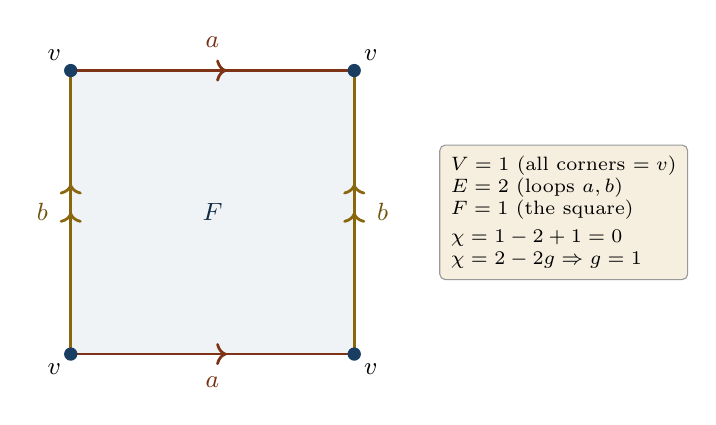
\begin{tikzpicture}[scale=1.2, every node/.style={font=\small}]
  % The identified square: bottom and top are edge a, left and right are edge b
  \coordinate (BL) at (0,0);
  \coordinate (BR) at (3,0);
  \coordinate (TR) at (3,3);
  \coordinate (TL) at (0,3);
  \fill[formteal!7] (BL) -- (BR) -- (TR) -- (TL) -- cycle;
  % edge a: bottom and top, single arrow
  \draw[postaction={decorate, decoration={markings, mark=at position 0.55 with {\arrow[draw=formrust!75!black]{>}}}}, formrust!75!black, line width=1pt] (BL) -- (BR);
  \draw[postaction={decorate, decoration={markings, mark=at position 0.55 with {\arrow[draw=formrust!75!black]{>}}}}, formrust!75!black, line width=1pt] (TL) -- (TR);
  % edge b: left and right, double arrow
  \draw[postaction={decorate, decoration={markings, mark=at position 0.5 with {\arrow[draw=formgold!75!black]{>}}, mark=at position 0.6 with {\arrow[draw=formgold!75!black]{>}}}}, formgold!75!black, line width=1pt] (BL) -- (TL);
  \draw[postaction={decorate, decoration={markings, mark=at position 0.5 with {\arrow[draw=formgold!75!black]{>}}, mark=at position 0.6 with {\arrow[draw=formgold!75!black]{>}}}}, formgold!75!black, line width=1pt] (BR) -- (TR);
  % all four corners are the single vertex v
  \foreach \p in {BL,BR,TR,TL}{\fill[formteal!80!black] (\p) circle (2pt);}
  \node[below left]  at (BL) {$v$};
  \node[below right] at (BR) {$v$};
  \node[above right] at (TR) {$v$};
  \node[above left]  at (TL) {$v$};
  \node[formrust!70!black] at (1.5,-0.3) {$a$};
  \node[formrust!70!black] at (1.5,3.3)  {$a$};
  \node[formgold!60!black] at (-0.3,1.5) {$b$};
  \node[formgold!60!black] at (3.3,1.5)  {$b$};
  \node[formteal!55!black] at (1.5,1.5) {$F$};
  % Count annotation
  \node[draw=black!40, rounded corners=2pt, fill=formivory, align=left,
        inner sep=4pt, font=\scriptsize, anchor=west] at (3.9,1.5)
    {$V = 1$ (all corners $= v$)\\
     $E = 2$ (loops $a, b$)\\
     $F = 1$ (the square)\\[2pt]
     $\chi = 1 - 2 + 1 = 0$\\
     $\chi = 2 - 2g \Rightarrow g = 1$};
\end{tikzpicture}
\caption{The CW structure on the torus. Gluing the two \(a\)-edges and the two
\(b\)-edges of the square sends all four corners to one vertex \(v\), leaves two
edge-loops \(a, b\), and one \(2\)-cell \(F\); hence \(\chi(T) = 0\) and
\(g = 1\).}
\label{fig:cwtorus}
\end{figure}

\begin{remark}
\label{rem:tg-genus-matters}
The genus is the one topological number that controls the function theory of a
compact Riemann surface. For genus one the Riemann--Roch theorem
(\cref{ch:riemann_roch}) takes the especially clean form \(\ell(D) = \deg D\) for
divisors of positive degree, and it is this that pins down the dimensions of the
spaces of functions used to build \(\wp\) and \(\wp'\). Everything downstream
rests on \(g = 1\).
\end{remark}

\section{Topological versus Complex Structure}
\label{sec:tg-top-vs-complex}

It is worth separating clearly the two layers we have placed on \(T\).

\begin{itemize}
\item \textbf{Topological / smooth layer (the same for all \(\Lambda\)).} By
\cref{cor:tg-abelian} every complex torus is, as a topological group, the single
object \(S^1 \times S^1\); by \cref{prop:tg-euler} it has genus one. No invariant
at this level distinguishes one lattice from another --- all complex tori are
diffeomorphic.

\item \textbf{Complex-analytic layer (depends on \(\Lambda\)).} The holomorphic
structure of \cref{thm:lat-riemann-surface} is extra data. By
\cref{prop:lat-normal-form} it is recorded, up to isomorphism, by the point
\(\tau \in \HH\) modulo \(\mathrm{SL}_2(\Z)\); two tori \(\C/\Lambda\) and
\(\C/\Lambda'\) are biholomorphic if and only if their \(\tau\)-classes agree.
\end{itemize}

Thus the diffeomorphism type is rigid (one torus) while the biholomorphism type
varies in the one-parameter family \(\HH / \mathrm{SL}_2(\Z)\). The single
complex number that separates the classes is the \(j\)-invariant of
\cref{ch:synthesis}. \Cref{warn:tg-not-biholo} is the concrete face of this: the
real coordinates \((s,t)\) trivialize \(T\) topologically but are blind to the
complex structure that the rest of the book exploits.

\section{Summary}
\label{sec:tg-summary}

The torus \(T = \C/\Lambda\) is an abelian group under \([u]+[v]=[u+v]\), with
holomorphic addition and negation, so it is a complex Lie group on which the
translations act simply transitively (\cref{prop:tg-welldef,prop:tg-lie}). As a
topological group it is \(S^1 \times S^1\), which makes commutativity visibly the
commutativity of adding angles, but this identification is only real-analytic and
forgets the complex structure (\cref{prop:tg-s1xs1,warn:tg-not-biholo}). A CW
decomposition gives \(\chi(T) = 0\) and genus \(g = 1\)
(\cref{prop:tg-euler}), the topological fact behind the simple form of
Riemann--Roch. All complex tori share this topology; what varies is the complex
structure, recorded by \(\tau \in \HH/\mathrm{SL}_2(\Z)\).

\section*{Exercises}
\addcontentsline{toc}{section}{Exercises}

\begin{exercise}
\label{ex:tg-lie-holo}
Complete the details of \cref{prop:tg-lie}: writing the addition map in two
overlapping charts of \cref{thm:lat-riemann-surface}, verify explicitly that the
transition makes \(m : T \times T \to T\) holomorphic, and deduce that
\(\iota([z]) = [-z]\) is biholomorphic.
\end{exercise}

\begin{exercise}
\label{ex:tg-two-torsion}
Show that the negation map \(\iota([z]) = [-z]\) has exactly four fixed points on
\(T\), namely
\[
  [0],\quad \Bigl[\tfrac{\omega_1}{2}\Bigr],\quad
  \Bigl[\tfrac{\omega_2}{2}\Bigr],\quad
  \Bigl[\tfrac{\omega_1+\omega_2}{2}\Bigr].
\]
These are the \emph{two-torsion} points, the solutions of \(2[z] = [0]\); they
reappear as the branch points of \(\wp\) in \cref{ch:embedding} and as the
two-torsion of the group law in \cref{ch:chord_tangent_cases}.
\end{exercise}

\begin{exercise}
\label{ex:tg-first-iso}
Fill in the first-isomorphism-theorem argument for \(\R/\Z \cong S^1\): check
that \(t \mapsto e^{2\pi i t}\) is a continuous surjective homomorphism with
kernel \(\Z\), and that the induced bijection \(\R/\Z \to S^1\) is a
homeomorphism (use compactness of \([0,1]\)).
\end{exercise}

\begin{exercise}
\label{ex:tg-euler-refine}
Recompute \(\chi(T)\) using a finer CW structure --- for instance subdivide
\(P_\Lambda\) into two triangles before gluing --- and confirm you again obtain
\(\chi(T) = 0\), illustrating the invariance of the Euler characteristic.
\end{exercise}

\begin{exercise}
\label{ex:tg-homeo-not-biholo}
Show that \(\C/(\Z + \Z i)\) and \(\C/(\Z + \Z\,2i)\) are homeomorphic (indeed
diffeomorphic) as real surfaces. Granting the standard fact that the points
\(\tau = i\) and \(\tau = 2i\) lie in the closed fundamental domain
\(\{\,|\tau| \ge 1,\ |\operatorname{Re}\tau| \le \tfrac12\,\}\) of
\(\mathrm{SL}_2(\Z)\) and are not identified by it, conclude (using
\cref{ch:lattices}) that the two tori are \emph{not} biholomorphic. Explain why
this does not contradict \cref{cor:tg-abelian}.
\end{exercise}


\part{Elliptic Functions}
% Elliptic Functions and Liouville's Theorems  (source §4, major expansion:
% the field of elliptic functions, no nonconstant holomorphic ones, and the
% three Liouville theorems -- residue sum, the valence/counting theorem, and the
% Abel relation sum(zeros) - sum(poles) in Lambda -- by contour integration over
% a period parallelogram)
\chapter{Elliptic Functions and Liouville's Theorems}
\label{ch:elliptic_liouville}

By \cref{rem:lat-translation-holo}, meromorphic functions on the torus
\(T = \C/\Lambda\) are the same as \(\Lambda\)-periodic meromorphic functions on
\(\C\) --- the \emph{elliptic functions}. This chapter establishes the rigid
constraints these functions obey. There are no nonconstant holomorphic ones, so
a nonconstant elliptic function must have poles; and the location and number of
its zeros and poles are governed by three theorems of Liouville, all proved by
integrating around a single period parallelogram. The third of them,
\(\sum(\text{zeros}) - \sum(\text{poles}) \in \Lambda\), is the analytic engine
of the entire group law: it returns in \cref{ch:abel} as Abel's sum law and is
what ultimately forces \(P + Q + R = O\) for collinear points in
\cref{thm:main}.

\section{The Field of Elliptic Functions}
\label{sec:ell-field}

\begin{definition}
\label{def:ell-elliptic}
A meromorphic function \(f\) on \(\C\) is \emph{elliptic} with respect to
\(\Lambda\), or \(\Lambda\)-periodic, if
\[
  f(z + \lambda) = f(z) \qquad \text{for all } \lambda \in \Lambda .
\]
Equivalently, \(f(z+\omega_1) = f(z)\) and \(f(z+\omega_2) = f(z)\) for a basis
\(\omega_1, \omega_2\).
\end{definition}

An elliptic function depends only on the class \([z]\), so it descends to a
meromorphic function \(T \to \CP^1\); conversely every meromorphic function on
\(T\) pulls back along \(\pi\) to a \(\Lambda\)-periodic one. The two viewpoints
are interchangeable, and we pass between them freely:
\[
  \{\text{meromorphic functions on } T\}
  \;\longleftrightarrow\;
  \{\Lambda\text{-elliptic functions on } \C\}.
\]

\begin{proposition}
\label{prop:ell-field}
The \(\Lambda\)-elliptic functions form a field, closed under differentiation:
if \(f, g\) are elliptic then so are \(f \pm g\), \(fg\), \(f/g\) (for
\(g \not\equiv 0\)), and \(f'\).
\end{proposition}

\begin{proof}
Sums, products, and quotients of meromorphic functions are meromorphic, and each
inherits \(\Lambda\)-periodicity pointwise, e.g.\ \((fg)(z+\lambda) =
f(z+\lambda)g(z+\lambda) = f(z)g(z)\). Differentiating \(f(z+\lambda)=f(z)\) in
\(z\) gives \(f'(z+\lambda) = f'(z)\), so \(f'\) is elliptic.
\end{proof}

The central problem of the theory is to describe this field. The answer,
reached in \cref{ch:weierstrass_wp}, is that it is generated by the Weierstrass
function \(\wp\) and its derivative \(\wp'\). Everything in this chapter is a
constraint that the generators must satisfy.

\section{No Nonconstant Holomorphic Elliptic Functions}
\label{sec:ell-liouville-const}

\begin{theorem}[Liouville's first theorem]
\label{thm:ell-const}
An elliptic function with no poles is constant.
\end{theorem}

\begin{proof}
Let \(f\) be elliptic and holomorphic on all of \(\C\). The closed fundamental
parallelogram
\(\overline{P} = \{ s\omega_1 + t\omega_2 : 0 \le s, t \le 1 \}\) is compact, so
the continuous function \(|f|\) attains a maximum \(M\) on \(\overline{P}\). By
periodicity every \(z \in \C\) is congruent to a point of \(\overline P\) and
\(f\) takes the same value there, so \(|f(z)| \le M\) for all \(z\): the entire
function \(f\) is bounded. By Liouville's theorem (a bounded entire function is
constant) \(f\) is constant. Equivalently, \(T\) is compact, so a holomorphic
\(f : T \to \C\) attains its maximum modulus and is constant by the maximum
modulus principle.
\end{proof}

Thus a nonconstant elliptic function must have at least one pole. The
quantitative versions of this statement are Liouville's remaining theorems.

\section{Integration Around a Period Parallelogram}
\label{sec:ell-contour}

All three theorems rest on one device. Fix a basis \(\omega_1, \omega_2\) and a
base point \(a \in \C\), and let
\[
  P_a = \{\, a + s\omega_1 + t\omega_2 : 0 \le s, t \le 1 \,\}
\]
be the translated fundamental parallelogram, with boundary \(\partial P_a\)
traversed counterclockwise. Because a nonconstant elliptic function has only
finitely many zeros and poles modulo \(\Lambda\), we may always choose \(a\) so
that \(\partial P_a\) passes through none of them
(\cref{fig:periodcontour}). Label the four sides
\[
  \mathrm{I}: a \to a{+}\omega_1, \quad
  \mathrm{II}: a{+}\omega_1 \to a{+}\omega_1{+}\omega_2, \quad
  \mathrm{III}: a{+}\omega_1{+}\omega_2 \to a{+}\omega_2, \quad
  \mathrm{IV}: a{+}\omega_2 \to a .
\]

\begin{figure}[ht]
\centering
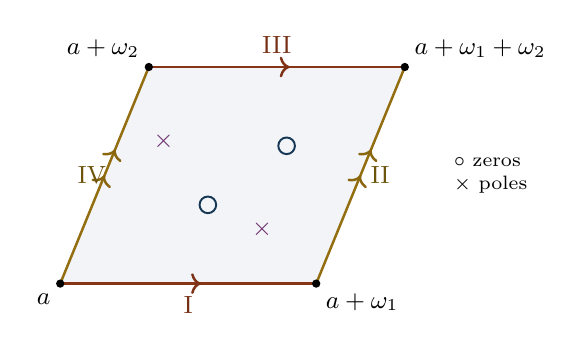
\begin{tikzpicture}[scale=1.25, every node/.style={font=\small}]
  \coordinate (A)  at (0,0);
  \coordinate (B)  at (2.6,0);       % a + w1
  \coordinate (C)  at (3.5,2.2);     % a + w1 + w2
  \coordinate (D)  at (0.9,2.2);     % a + w2
  \fill[formteal!6] (A) -- (B) -- (C) -- (D) -- cycle;
  % side I (bottom) and III (top): direction-matched single arrows
  \draw[postaction={decorate, decoration={markings, mark=at position 0.55 with {\arrow[draw=formrust!75!black]{>}}}}, formrust!80!black, line width=0.9pt] (A) -- (B);
  \draw[postaction={decorate, decoration={markings, mark=at position 0.55 with {\arrow[draw=formrust!75!black]{>}}}}, formrust!80!black, line width=0.9pt] (D) -- (C);
  % side II (right) and IV (left): double arrows
  \draw[postaction={decorate, decoration={markings, mark=at position 0.5 with {\arrow[draw=formgold!75!black]{>}}, mark=at position 0.62 with {\arrow[draw=formgold!75!black]{>}}}}, formgold!80!black, line width=0.9pt] (B) -- (C);
  \draw[postaction={decorate, decoration={markings, mark=at position 0.5 with {\arrow[draw=formgold!75!black]{>}}, mark=at position 0.62 with {\arrow[draw=formgold!75!black]{>}}}}, formgold!80!black, line width=0.9pt] (A) -- (D);
  % vertices
  \foreach \p in {A,B,C,D}{\fill[black] (\p) circle (1.2pt);}
  \node[below left]  at (A) {$a$};
  \node[below right] at (B) {$a+\omega_1$};
  \node[above right] at (C) {$a+\omega_1+\omega_2$};
  \node[above left]  at (D) {$a+\omega_2$};
  \node[formrust!70!black] at (1.3,-0.22) {I};
  \node[formrust!70!black] at (2.2,2.42) {III};
  \node[formgold!60!black] at (3.25,1.1) {II};
  \node[formgold!60!black] at (0.32,1.1) {IV};
  % some zeros (open) and poles (cross) inside
  \draw[formteal!70!black, line width=0.7pt] (1.5,0.8) circle (2.4pt);
  \draw[formteal!70!black, line width=0.7pt] (2.3,1.4) circle (2.4pt);
  \node[formplum] at (1.05,1.45) {$\times$};
  \node[formplum] at (2.05,0.55) {$\times$};
  \node[font=\scriptsize, anchor=west, align=left] at (3.9,1.1)
    {$\circ$ zeros\\ $\times$ poles};
\end{tikzpicture}
\caption{A period parallelogram \(P_a\), chosen so its boundary avoids the zeros
(\(\circ\)) and poles (\(\times\)) of \(f\). For an elliptic integrand the
integral over side III cancels that over side I (they are translates by
\(\omega_2\) traversed oppositely), and II cancels IV; the boundary integral
vanishes.}
\label{fig:periodcontour}
\end{figure}

\begin{lemma}[Opposite sides cancel]
\label{lem:ell-cancel}
If \(g\) is elliptic and has no poles on \(\partial P_a\), then
\(\oint_{\partial P_a} g(z)\,dz = 0\).
\end{lemma}

\begin{proof}
Side \(\mathrm{III}\) is the translate of side \(\mathrm{I}\) by \(\omega_2\),
traversed in the opposite direction. Substituting \(z = w + \omega_2\) and using
\(g(w+\omega_2) = g(w)\),
\[
  \int_{\mathrm{III}} g\,dz
  = -\int_{\mathrm{I}} g(w+\omega_2)\,dw
  = -\int_{\mathrm{I}} g(w)\,dw ,
\]
so \(\int_{\mathrm{I}} + \int_{\mathrm{III}} = 0\). Likewise side
\(\mathrm{II}\) is the translate of side \(\mathrm{IV}\) by \(\omega_1\), traversed
oppositely, so \(\int_{\mathrm{II}} + \int_{\mathrm{IV}} = 0\). Adding gives
\(\oint_{\partial P_a} g\,dz = 0\).
\end{proof}

\section{Liouville's Theorems}
\label{sec:ell-liouville}

\subsection{The sum of residues vanishes}

\begin{theorem}[Liouville's second theorem: residues]
\label{thm:ell-residues}
For a nonconstant elliptic function \(f\), the sum of the residues over one
period parallelogram is zero:
\[
  \sum_{[p] \in T} \Res_{p} f = 0 .
\]
\end{theorem}

\begin{proof}
Choose \(a\) so that \(\partial P_a\) avoids the poles of \(f\). The interior of
\(P_a\) contains exactly one representative of each pole class. By the residue
theorem and \cref{lem:ell-cancel} applied to \(g = f\),
\[
  2\pi i \sum_{p \in P_a} \Res_p f
  = \oint_{\partial P_a} f(z)\,dz = 0 . \qedhere
\]
\end{proof}

\begin{corollary}
\label{cor:ell-order2}
No elliptic function has a single simple pole in a period parallelogram. The
\emph{order} of a nonconstant elliptic function --- the number of poles, counted
with multiplicity, in one period parallelogram --- is at least \(2\).
\end{corollary}

\begin{proof}
A function with one simple pole and no others would have a single nonzero
residue, contradicting \cref{thm:ell-residues}. So either there are at least two
poles, or a single pole of order \(\ge 2\); in both cases the order is at least
\(2\).
\end{proof}

This is the first hint of the Weierstrass function: the smallest a nonconstant
elliptic function can be is order two, realized by a single double pole. That
function is \(\wp\) (\cref{ch:weierstrass_wp}).

\subsection{The counting theorem}

\begin{theorem}[Liouville's third theorem: valence]
\label{thm:ell-valence}
A nonconstant elliptic function \(f\) of order \(N\) has exactly \(N\) zeros and
\(N\) poles in each period parallelogram, counted with multiplicity. More
generally, for every \(c \in \CP^1\) the equation \(f(z) = c\) has exactly \(N\)
solutions there; \(f : T \to \CP^1\) is an \(N\)-to-one branched cover.
\end{theorem}

\begin{proof}
The logarithmic derivative \(f'/f\) is elliptic by \cref{prop:ell-field}, with a
simple pole at each zero and pole of \(f\); its residue there is
\(\Res_p(f'/f) = \ord_p(f)\). Choosing \(a\) so \(\partial P_a\) avoids these
points, \cref{lem:ell-cancel} and the residue theorem give
\[
  0 = \oint_{\partial P_a} \frac{f'}{f}\,dz
  = 2\pi i \sum_{p \in P_a} \ord_p(f)
  = 2\pi i \bigl( Z - P \bigr),
\]
where \(Z\) and \(P\) are the numbers of zeros and poles with multiplicity.
Hence \(Z = P = N\). Applying this to \(f - c\) (also elliptic, of order \(N\),
with the same poles as \(f\)) shows \(f - c\) has \(N\) zeros, i.e.\ \(f\) takes
the value \(c\) exactly \(N\) times; the case \(c = \infty\) is the pole count.
\end{proof}

\subsection{The Abel relation}

The previous theorems used elliptic integrands. The decisive third statement
uses \(z\,f'(z)/f(z)\), whose factor \(z\) is \emph{not} periodic; the failure of
cancellation is precisely a lattice vector.

\begin{theorem}[Liouville's fourth theorem: the Abel relation]
\label{thm:ell-abel}
Let \(f\) be a nonconstant elliptic function. Listing its zeros \(z_1, \dots,
z_N\) and poles \(p_1, \dots, p_N\) in a period parallelogram with multiplicity,
\[
  \sum_{k=1}^{N} z_k \;-\; \sum_{k=1}^{N} p_k \;\in\; \Lambda .
\]
Equivalently, in the group \(T\), \(\sum_k [z_k] = \sum_k [p_k]\).
\end{theorem}

\begin{proof}
Consider \(g(z) = z\,f'(z)/f(z)\). At a zero or pole \(p\) of \(f\) of order
\(m = \ord_p(f)\) one has \(f'/f \sim m/(z-p)\), so \(\Res_p g = m\,p\). With
\(\partial P_a\) avoiding the zeros and poles, the residue theorem gives
\[
  \oint_{\partial P_a} g(z)\,dz
  = 2\pi i \sum_{p \in P_a} \ord_p(f)\, p
  = 2\pi i\Bigl( \sum_k z_k - \sum_k p_k \Bigr).
\tag{$\ast$}
\]
Now evaluate the contour integral directly, pairing opposite sides. On side
\(\mathrm{III}\) put \(z = w + \omega_2\) with \(w\) running along
\(\mathrm{I}\) reversed; since \(f'/f\) is \(\omega_2\)-periodic,
\[
  \int_{\mathrm{I}} + \int_{\mathrm{III}}
  = \int_{\mathrm{I}} \bigl[\, z - (z+\omega_2) \,\bigr]\frac{f'}{f}\,dz
  = -\,\omega_2 \int_{a}^{a+\omega_1} \frac{f'}{f}\,dz .
\]
The remaining integral is the change in \(\log f\) along side \(\mathrm{I}\);
because \(f(a+\omega_1) = f(a)\), this change is \(2\pi i\,k_1\) for some integer
\(k_1\) (the winding number of \(f\) along the side). Thus
\(\int_{\mathrm{I}} + \int_{\mathrm{III}} = -2\pi i\,k_1\,\omega_2\). Symmetrically,
pairing \(\mathrm{II}\) with \(\mathrm{IV}\) and using
\(\omega_1\)-periodicity,
\[
  \int_{\mathrm{II}} + \int_{\mathrm{IV}}
  = \omega_1 \int_{a}^{a+\omega_2} \frac{f'}{f}\,dz
  = 2\pi i\,k_2\,\omega_1
\]
for an integer \(k_2\). Adding,
\[
  \oint_{\partial P_a} g\,dz = 2\pi i\,( k_2\,\omega_1 - k_1\,\omega_2 ).
\tag{$\ast\ast$}
\]
Comparing \((\ast)\) and \((\ast\ast)\) and cancelling \(2\pi i\),
\[
  \sum_k z_k - \sum_k p_k = k_2\,\omega_1 - k_1\,\omega_2 \in \Lambda . \qedhere
\]
\end{proof}

\begin{keyidea}{The relation behind the group law}
\Cref{thm:ell-abel} says: for any elliptic function, the zeros and poles, added
as points of \(T\), are equal. Read backward it is a recipe --- if a divisor of
points has zero degree and its points sum to \(0\) in \(T\), it is the divisor of
an elliptic function (\cref{ch:riemann_roch} supplies the converse). When the
points are the intersections of the cubic with a line, this congruence becomes
\(P + Q + R = O\). The chord--tangent law is \cref{thm:ell-abel} in disguise.
\end{keyidea}

\section{Consequences and the Road Ahead}
\label{sec:ell-consequences}

The four theorems pin down the coarse shape of every elliptic function:

\begin{itemize}
\item it has no poles only if it is constant (\cref{thm:ell-const});
\item its residues sum to zero, so it cannot have order one
  (\cref{thm:ell-residues,cor:ell-order2});
\item it attains every value the same number \(N \ge 2\) of times
  (\cref{thm:ell-valence});
\item its zeros and poles satisfy \(\sum z_k \equiv \sum p_k \pmod \Lambda\)
  (\cref{thm:ell-abel}).
\end{itemize}

The minimal case \(N = 2\) is therefore the place to look for a generator of the
field. A function with a single double pole at \([0]\) would, by
\cref{thm:ell-valence}, have two zeros, and by \cref{thm:ell-abel} those zeros
\(z_1, z_2\) would satisfy \(z_1 + z_2 \equiv 0\), i.e.\ \(z_2 \equiv -z_1\):
the zeros are antipodal. This is exactly the behaviour of \(\wp - c\), and it is
why \(\wp\) is an even function. Whether such a function exists at all is a
dimension count, answered by Riemann--Roch in \cref{ch:riemann_roch}; its
explicit construction is \cref{ch:weierstrass_wp}.

\section{Summary}
\label{sec:ell-summary}

Elliptic functions are the meromorphic functions on \(T\); they form a
differential field. A nonconstant one must have poles (\cref{thm:ell-const}), of
total order \(N \ge 2\) (\cref{cor:ell-order2}), and it takes every value exactly
\(N\) times (\cref{thm:ell-valence}). Integrating \(f\), \(f'/f\), and
\(z\,f'/f\) around a period parallelogram yields, respectively, the vanishing of
the residue sum, the equality of zero and pole counts, and the Abel relation
\(\sum(\text{zeros}) - \sum(\text{poles}) \in \Lambda\)
(\cref{thm:ell-residues,thm:ell-valence,thm:ell-abel}). The last is the analytic
heart of the group law and reappears as Abel's sum law in \cref{ch:abel}.

\section*{Exercises}
\addcontentsline{toc}{section}{Exercises}

\begin{exercise}
\label{ex:ell-field}
Verify in detail that the \(\Lambda\)-elliptic functions form a field closed
under \(d/dz\) (\cref{prop:ell-field}). Show in addition that if \(f\) is
elliptic then so is \(f(z+a)\) for any fixed \(a \in \C\), and that an even
elliptic function (\(f(-z) = f(z)\)) has \(f'\) odd.
\end{exercise}

\begin{exercise}
\label{ex:ell-no-order-one}
Give a complete proof that there is no elliptic function of order one. Then show
that an elliptic function of order two has either two distinct simple poles with
opposite residues, or a single double pole with residue zero.
\end{exercise}

\begin{exercise}
\label{ex:ell-double-pole-zeros}
Suppose \(f\) is elliptic of order two with a single double pole at \([0]\).
Using \cref{thm:ell-valence,thm:ell-abel}, show that the two zeros of \(f\) are
of the form \([w]\) and \([-w]\) for some \(w\). Conclude that \(f(z) - f(z_0)\)
has zeros at \(\pm z_0\) for generic \(z_0\), the signature of an even function.
\end{exercise}

\begin{exercise}
\label{ex:ell-sum-values}
Let \(f\) be elliptic of order \(N\) and let \(c_1, c_2 \in \C\) be two values.
Using \cref{thm:ell-abel} applied to \(f - c_1\) and to \(f - c_2\), show that
the sum of the \(N\) solutions of \(f(z) = c_1\) equals, modulo \(\Lambda\), the
sum of the \(N\) solutions of \(f(z) = c_2\). (The common value is an invariant
of \(f\).)
\end{exercise}

\begin{exercise}
\label{ex:ell-winding}
In the proof of \cref{thm:ell-abel} the integers \(k_1, k_2\) are winding
numbers of \(f\) along the two sides of \(P_a\). Show directly that
\(\int_a^{a+\omega_1} (f'/f)\,dz \in 2\pi i\,\Z\) whenever \(f(a+\omega_1) =
f(a)\) and \(f\) has no zeros or poles on the segment, and interpret \(k_1\) as
the number of times \(f\) winds around \(0\).
\end{exercise}

% Divisors and the Degree-Zero Theorem  (source §5; added: the divisor group
% Div(X), degree homomorphism, linear equivalence and Pic^0, and the Abel-sum
% map Div^0(T) -> T with Pic^0(T) =~ T)
\chapter{Divisors and the Degree-Zero Theorem}
\label{ch:divisors}

\Cref{ch:elliptic_liouville} controlled the zeros and poles of a single elliptic
function. Divisors are the bookkeeping that turns those zero/pole data into an
algebraic object one can add and compare. On a compact Riemann surface the
divisor of a function has degree zero; on the torus it additionally has Abel sum
zero. Packaging these two constraints gives the \emph{Picard group}
\(\Pic^0(T)\) and a map \(\Pic^0(T) \to T\) that is the structural shadow of the
group law: when we later put a group law on the cubic, it will be exactly this
map.

\section{Orders and the Divisor of a Function}
\label{sec:div-orders}

Let \(X\) be a Riemann surface and \(f\) a nonzero meromorphic function. In a
local coordinate \(t\) centered at a point \(p\) we may write
\[
  f(t) = t^{m} u(t), \qquad u \text{ holomorphic}, \quad u(0) \ne 0 .
\]
The integer \(m\) is the \emph{order} of \(f\) at \(p\), written
\(\ord_p(f) = m\):
\[
  m > 0 \ \text{(zero of order } m),\qquad
  m = 0 \ \text{(finite, nonzero)},\qquad
  m < 0 \ \text{(pole of order } {-m}).
\]

\begin{remark}
\label{rem:div-ord-welldef}
The order does not depend on the chart. If \(s\) is another coordinate at
\(p\), then \(t = s\,h(s)\) with \(h\) holomorphic and \(h(0) \ne 0\), so
\(f = s^{m}\bigl(h(s)^{m} u(t(s))\bigr)\) and the new unit
\(h^{m}\,(u\circ t)\) is again nonvanishing at \(s=0\); the exponent \(m\) is
unchanged. Thus \(\ord_p(f)\) is intrinsic.
\end{remark}

\begin{definition}
\label{def:div-divisor-of-f}
The \emph{divisor} of a nonzero meromorphic function \(f\) is the formal sum
\[
  \divisor(f) = \sum_{p \in X} \ord_p(f)\, p .
\]
On a compact \(X\) only finitely many terms are nonzero, so this is a finite
sum.
\end{definition}

\section{The Divisor Group and Degree}
\label{sec:div-group}

\begin{definition}
\label{def:div-group}
A \emph{divisor} on \(X\) is a finite formal integer combination of points,
\[
  D = \sum_{p \in X} n_p\, p, \qquad n_p \in \Z, \ \ n_p = 0 \text{ for all but finitely many } p .
\]
Under coefficientwise addition the divisors form the free abelian group
\(\Div(X)\) on the points of \(X\). The \emph{degree} is the homomorphism
\[
  \degdiv : \Div(X) \to \Z, \qquad \degdiv\Bigl( \sum_p n_p\, p \Bigr) = \sum_p n_p .
\]
A divisor of the form \(\divisor(f)\) is called \emph{principal}; we write
\(\Prin(X)\) for the set of principal divisors.
\end{definition}

\begin{proposition}
\label{prop:div-prin-subgroup}
The principal divisors form a subgroup of \(\Div(X)\): for nonzero meromorphic
\(f, g\),
\[
  \divisor(fg) = \divisor(f) + \divisor(g),
  \qquad
  \divisor(1/f) = -\divisor(f),
\]
and \(\divisor(c) = 0\) for a nonzero constant \(c\).
\end{proposition}

\begin{proof}
Orders add under multiplication: \(\ord_p(fg) = \ord_p(f) + \ord_p(g)\), directly
from \(f = t^{m}u\), \(g = t^{n}v\) giving \(fg = t^{m+n}uv\). Summing over \(p\)
gives the first identity; the others are the cases \(g = 1/f\) and \(f = c\).
Hence \(\Prin(X)\) is closed under addition and negation, a subgroup.
\end{proof}

\section{Principal Divisors Have Degree Zero}
\label{sec:div-degzero}

The single most important property of principal divisors on a compact surface is
that they are invisible to the degree.

\begin{theorem}[Degree-zero theorem]
\label{thm:div-degzero}
If \(X\) is compact and \(f\) is a nonzero meromorphic function on \(X\), then
\[
  \degdiv \divisor(f) = 0 .
\]
\end{theorem}

\begin{proof}
Consider the meromorphic differential \(df/f\). Near \(p\), writing
\(f = t^{m} u\) with \(u(0) \ne 0\),
\[
  \frac{df}{f} = \frac{d(t^{m}u)}{t^{m}u}
  = m\,\frac{dt}{t} + \frac{du}{u},
\]
and the second term is holomorphic at \(p\). Hence \(df/f\) has at worst a simple
pole at \(p\), with
\[
  \Res_p\!\left( \frac{df}{f} \right) = m = \ord_p(f) .
\]
By the residue theorem on the compact Riemann surface \(X\) the sum of all
residues of the global differential \(df/f\) vanishes, so
\[
  0 = \sum_{p} \Res_p\!\left( \frac{df}{f} \right) = \sum_p \ord_p(f)
  = \degdiv \divisor(f) . \qedhere
\]
\end{proof}

\begin{keyidea}{What degree zero means}
A meromorphic function on a compact Riemann surface has as many zeros as poles,
counted with multiplicity --- the divisor form of the argument principle. On the
torus this is \cref{thm:ell-valence} with \(N = \deg(\text{pole divisor})\): the
two theorems are the same fact seen from the two sides of the
\(T \leftrightarrow \C\) dictionary.
\end{keyidea}

In particular \(\Prin(X) \subseteq \Div^0(X)\), where
\[
  \Div^0(X) = \ker(\degdiv) = \{ D : \degdiv D = 0 \}
\]
is the group of degree-zero divisors.

\section{Linear Equivalence and the Picard Group}
\label{sec:div-picard}

\begin{definition}
\label{def:div-lineq}
Two divisors \(D, D'\) are \emph{linearly equivalent}, written \(D \sim D'\), if
\(D - D'\) is principal. The quotient group
\[
  \Pic(X) = \Div(X)/\Prin(X)
\]
is the \emph{Picard group}, and the class of \(D\) is denoted \([D]\).
\end{definition}

Because principal divisors have degree zero (\cref{thm:div-degzero}), the degree
descends to a homomorphism \(\degdiv : \Pic(X) \to \Z\), and its kernel
\[
  \Pic^0(X) = \Div^0(X)/\Prin(X)
\]
is the \emph{degree-zero Picard group}. The size of \(\Pic^0\) measures how far
divisors of degree zero are from being principal --- equivalently, how many
meromorphic functions the surface admits. On \(\CP^1\) every degree-zero divisor
is principal and \(\Pic^0 = 0\); on the torus, as we now show, \(\Pic^0\) is as
large as \(T\) itself.

\section{The Abel--Jacobi Sum Map}
\label{sec:div-abel-jacobi}

Specialize to \(X = T = \C/\Lambda\). Here points of \(T\) are themselves group
elements, so a degree-zero divisor can be \emph{summed}.

\begin{definition}
\label{def:div-sigma}
The \emph{Abel--Jacobi sum map} is
\[
  \smap : \Div^0(T) \to T,
  \qquad
  \smap\Bigl( \sum_i n_i\,[z_i] \Bigr) = \sum_i n_i\,[z_i] \in T,
\]
where the right-hand sum is taken in the group \(T\).
\end{definition}

It is a group homomorphism, immediately from the definition. The content of the
previous chapter is exactly that \(\smap\) annihilates principal divisors.

\begin{proposition}
\label{prop:div-sigma-kills-prin}
For every nonzero elliptic function \(f\), \(\smap(\divisor f) = 0\). Hence
\(\smap\) descends to a homomorphism
\[
  \bar\smap : \Pic^0(T) \to T .
\]
\end{proposition}

\begin{proof}
Write \(\divisor(f) = \sum_k [z_k] - \sum_k [p_k]\) with the zeros and poles
listed by multiplicity; it has degree zero by \cref{thm:div-degzero} (or
\cref{thm:ell-valence}), so it lies in \(\Div^0(T)\). Then
\(\smap(\divisor f) = \sum_k [z_k] - \sum_k [p_k]\), which is \(0\) in \(T\) by
the Abel relation \cref{thm:ell-abel}. Since \(\smap\) kills the subgroup
\(\Prin(T)\), it factors through \(\Pic^0(T) = \Div^0(T)/\Prin(T)\).
\end{proof}

\begin{theorem}[Abel--Jacobi for the torus]
\label{thm:div-pic-iso}
The map \(\bar\smap : \Pic^0(T) \to T\) is an isomorphism of groups. In
particular every complex torus is its own \emph{Jacobian}:
\(\Pic^0(T) \cong T\).
\end{theorem}

\begin{proof}[Proof of surjectivity, and the standing of injectivity]
\emph{Surjectivity.} Given any \([a] \in T\), the divisor \([a] - [0]\) has degree
zero and \(\smap([a]-[0]) = [a] - [0] = [a]\). So \(\bar\smap\) hits every
element of \(T\).

\emph{Well-definedness and homomorphism} are \cref{prop:div-sigma-kills-prin}.

\emph{Injectivity} is the converse of Abel's relation: if \(D \in \Div^0(T)\)
has \(\smap(D) = 0\), then \(D\) is principal, i.e.\ \(D = \divisor(f)\) for some
elliptic \(f\). This requires \emph{constructing} an elliptic function with
prescribed zeros and poles, which we do not yet have the tools for. It follows
once the Weierstrass machinery is in place: \cref{ch:riemann_roch} produces
enough functions, and the explicit construction is carried out through
\crefrange{ch:weierstrass_wp}{ch:transport}. We therefore record injectivity
here and complete it there.
\end{proof}

\begin{keyidea}{Why this is the whole story}
\Cref{thm:div-pic-iso} says the degree-zero divisor classes on the torus
\emph{are} the points of the torus, via summation. Two divisors are linearly
equivalent precisely when their points have the same Abel sum. When we transport
the picture to the cubic \(E\) in \crefrange{ch:lines_divisors}{ch:transport},
the group law on \(E\) will be defined by linear equivalence of divisors --- and
by this theorem that is the same as addition on \(T\). The chord--tangent law is
the composite
\[
  E \;\cong\; T \;\xleftarrow{\ \bar\smap\ }\; \Pic^0(T) ,
\]
read as a single group.
\end{keyidea}

\section{Summary}
\label{sec:div-summary}

Divisors on \(X\) form the free abelian group \(\Div(X)\), graded by degree, with
the principal divisors \(\divisor(f)\) as a subgroup. On a compact surface every
principal divisor has degree zero (\cref{thm:div-degzero}), so degree descends to
the Picard group \(\Pic(X) = \Div(X)/\Prin(X)\) and cuts out \(\Pic^0(X)\). On
the torus the Abel--Jacobi map \(\smap : \Div^0(T) \to T\) sums a divisor's
points; it kills principal divisors by the Abel relation
(\cref{prop:div-sigma-kills-prin}), and the induced
\(\bar\smap : \Pic^0(T) \to T\) is an isomorphism (\cref{thm:div-pic-iso}, with
injectivity completed later). This identification \(\Pic^0(T) \cong T\) is the
algebraic form of the group law that the rest of the book transports to the
cubic.

\section*{Exercises}
\addcontentsline{toc}{section}{Exercises}

\begin{exercise}
\label{ex:div-hom}
Show that \(f \mapsto \divisor(f)\) is a homomorphism from the multiplicative
group of nonzero meromorphic functions to \(\Div(X)\), and that on a compact
\(X\) its kernel is exactly the nonzero constants. (Use
\cref{thm:div-degzero} and \cref{thm:ell-const} for the torus case.)
\end{exercise}

\begin{exercise}
\label{ex:div-ord-welldef}
Prove carefully that \(\ord_p(f)\) is independent of the local coordinate
(\cref{rem:div-ord-welldef}), and deduce that \(\ord_p(f+g) \ge
\min(\ord_p f, \ord_p g)\) with equality when the two orders differ.
\end{exercise}

\begin{exercise}
\label{ex:div-pic-split}
Using the base point \([0] \in T\), show that
\[
  \Div(T) \xrightarrow{\ \sim\ } \Z \oplus \Div^0(T),
  \qquad D \mapsto \bigl( \degdiv D,\ D - (\degdiv D)[0] \bigr),
\]
and deduce a splitting \(\Pic(T) \cong \Z \oplus \Pic^0(T)\). Combined with
\cref{thm:div-pic-iso}, conclude \(\Pic(T) \cong \Z \oplus T\).
\end{exercise}

\begin{exercise}
\label{ex:div-distinct-points}
Let \([a], [b] \in T\). Using the Abel relation \cref{thm:ell-abel}, prove that
the divisor \([a] - [b]\) is principal \emph{if and only if} \([a] = [b]\).
Contrast this with \(\CP^1\), where \emph{any} two points satisfy
\([a] - [b] = \divisor\!\bigl(\tfrac{z-a}{z-b}\bigr)\). Why does this recover
\cref{cor:ell-order2}?
\end{exercise}

\begin{exercise}
\label{ex:div-sigma-compute}
Take \(\Lambda = \Z + \Z\tau\) and the divisor
\(D = [\tfrac12] + [\tfrac{\tau}{2}] + [\tfrac{1+\tau}{2}] - 3\,[0]\). Compute
\(\degdiv D\) and \(\smap(D) \in T\). Is \(D\) a candidate for a principal
divisor? (Recall the two-torsion points from \cref{ex:tg-two-torsion}.)
\end{exercise}


\part{Riemann--Roch on Genus One}
% Riemann--Roch and Its Consequences  (source §6; restructured: the dimension
% counts that justify 1, wp, wp' are derived ELEMENTARILY from Chapter 4 plus the
% explicit Weierstrass functions, so the main line is self-contained; Riemann--Roch
% is kept as the general theorem (stated, cited) and is genuinely needed only for
% the converse of Abel / Pic^0(T) =~ T, which is off the critical path.)
\chapter{Riemann--Roch and Its Consequences}
\label{ch:riemann_roch}

We can now answer the question left open in \cref{ch:elliptic_liouville}: how
small can the pole divisor of a nonconstant elliptic function be? The answer is a
dimension count, and on the torus that count is \emph{elementary} --- it follows
from the Liouville theorems of \cref{ch:elliptic_liouville} together with the
explicit functions built in \cref{ch:weierstrass_wp}, with no appeal to a deep
theorem. We derive it that way first, because it is what justifies the functions
\(1, \wp, \wp'\) and carries the main argument. We then state the
\emph{Riemann--Roch} theorem in general, for context. The one auxiliary result it
might have supplied --- the converse of Abel's law, \(\Pic^0(T) \cong T\) --- is
instead proved constructively in \cref{ch:weierstrass_wp} with the
\(\sigma\)-function, so Riemann--Roch is needed nowhere and appears only as the
general theorem behind the elementary counts.

\section{The Spaces \texorpdfstring{$L(D)$}{L(D)}}
\label{sec:rr-spaces}

We order divisors by \(D \ge 0\) iff every coefficient of \(D\) is
nonnegative (an \emph{effective} divisor), and \(D \ge D'\) iff \(D - D' \ge 0\).

\begin{definition}
\label{def:rr-LD}
For a divisor \(D\) on a compact Riemann surface \(X\),
\[
  L(D) = \{ f \in \M(X) : \divisor(f) + D \ge 0 \} \cup \{0\},
  \qquad \ell(D) = \dim_\C L(D) .
\]
The condition \(\divisor(f) + D \ge 0\) says \(f\) may have a pole of order at
most \(n_p\) where \(D = \sum n_p\,p\) has \(n_p > 0\), and must have a zero of
order at least \(-n_p\) where \(n_p < 0\). For \(D = nO\) with \(n \ge 0\),
\(L(nO)\) is the space of functions whose only pole is at \(O\), of order at most
\(n\).
\end{definition}

\begin{proposition}[Elementary properties of \texorpdfstring{$L(D)$}{L(D)}]
\label{prop:rr-LD-props}
Let \(D, D'\) be divisors on a compact Riemann surface \(X\).
\begin{enumerate}
\item \(L(D)\) is a \(\C\)-vector space, and \(\ell(0) = 1\) with \(L(0) = \C\).
\item If \(D \le D'\) then \(L(D) \subseteq L(D')\) and
  \(\ell(D') - \ell(D) \le \deg(D' - D)\).
\item If \(\deg D < 0\) then \(L(D) = 0\), so \(\ell(D) = 0\).
\item Linearly equivalent divisors have isomorphic spaces: \(D \sim D'\) implies
  \(L(D) \cong L(D')\), so \(\ell\) depends only on the class \([D]\).
\end{enumerate}
\end{proposition}

\begin{proof}
(1) If \(\divisor(f) + D \ge 0\) and \(\divisor(g) + D \ge 0\) then for
\(a, b \in \C\), \(\ord_p(af+bg) \ge \min(\ord_p f, \ord_p g) \ge -n_p\)
(\cref{ex:div-ord-welldef}), so \(af + bg \in L(D)\). For \(D = 0\), \(L(0)\) is
the holomorphic functions on \(X\), which are the constants by
\cref{thm:ell-const} (compactness), so \(\ell(0) = 1\).

(2) The inclusion is immediate from \(\divisor(f) + D \le \divisor(f) + D'\).
Writing \(D' = D + \sum_j p_j\) with \(\deg(D'-D)\) points (with multiplicity),
each added point relaxes the pole bound at \(p_j\) by one, and the map sending
\(f\) to its Laurent coefficient of that extra allowed order is linear; its
kernel is the smaller space, so the dimension grows by at most one per point.

(3) A nonzero \(f \in L(D)\) has \(\divisor(f) \ge -D\), so
\(0 = \deg\divisor(f) \ge -\deg D\) by \cref{thm:div-degzero}; thus
\(\deg D \ge 0\). Contrapositively \(\deg D < 0\) forces \(L(D) = 0\).

(4) If \(D' = D + \divisor(h)\), then \(f \mapsto f/h\) is a linear isomorphism
\(L(D) \to L(D')\), since \(\divisor(f/h) + D' = \divisor(f) + D \ge 0\).
\end{proof}

\section{The Dimension Counts, Elementarily}
\label{sec:rr-counts}

The counts that the rest of the book uses --- \(\ell(O) = 1\), \(\ell([a]) = 1\),
and \(\ell(nO) = n\) --- need nothing beyond \cref{ch:elliptic_liouville} and the
explicit functions of \cref{ch:weierstrass_wp}.

\begin{proposition}[Dimension counts on the torus]
\label{prop:rr-counts}
On \(T = \C/\Lambda\):
\begin{enumerate}
\item \(\ell(O) = 1\), and \(\ell([a]) = 1\) for every single point \([a]\);
\item \(\ell(nO) \le n\) for all \(n \ge 1\);
\item \(\ell(nO) = n\) for all \(n \ge 1\).
\end{enumerate}
\end{proposition}

\begin{proof}
(1) A nonzero \(f \in L([a])\) has at most a simple pole at \([a]\) and no other
poles, so it is an elliptic function of order at most one. By
\cref{cor:ell-order2} there is no elliptic function of order exactly one, so \(f\)
is holomorphic, hence constant (\cref{thm:ell-const}); thus \(\ell([a]) = 1\).
The case \([a] = O\) is the same.

(2) By the point lemma \(\ell(D + p) - \ell(D) \in \{0,1\}\)
(\cref{ex:rr-point-lemma}), applied \(n-1\) times starting from \(\ell(O) = 1\),
\[
  \ell(nO) \le \ell(O) + (n-1) = n .
\]

(3) For the matching lower bound we exhibit \(n\) independent elements of
\(L(nO)\). \Cref{ch:weierstrass_wp} constructs the elliptic functions \(\wp\)
(a double pole at \(O\), order \(2\)) and \(\wp'\) (a triple pole, order \(3\)).
The functions
\[
  1, \quad \wp^{a}\ (a \ge 1),\quad \wp^{a}\wp'\ (a \ge 0)
\]
have poles only at \(O\), of orders \(0\) and \(2a\) and \(2a+3\) respectively, so
they realize every pole order in \(\{0, 2, 3, 4, \dots, n\}\) --- that is \(n\)
distinct orders, hence \(n\) linearly independent members of \(L(nO)\). Therefore
\(\ell(nO) \ge n\), and with (2), \(\ell(nO) = n\).
\end{proof}

\begin{remark}
\label{rem:rr-elementary}
The proof used only the Liouville theorems of \cref{ch:elliptic_liouville}
(\cref{cor:ell-order2,thm:ell-const}), the degree-zero theorem
(\cref{thm:div-degzero}, via the point lemma), and the existence of \(\wp, \wp'\)
from \cref{ch:weierstrass_wp}. No Riemann--Roch is needed. The same argument gives
\(\ell([a]) = 1\) for any point, which is all the converse of Abel will require of
these counts.
\end{remark}

\section{The Canonical Divisor of a Torus}
\label{sec:rr-canonical}

For the general theorem we need the \emph{canonical divisor} \(K\), the divisor of
any nonzero meromorphic \(1\)-form. On a compact surface of genus \(g\) all such
forms are linearly equivalent and \(\deg K = 2g - 2\). For the torus the canonical
class is trivial.

\begin{proposition}
\label{prop:rr-canonical}
On \(T = \C/\Lambda\) the holomorphic \(1\)-form \(dz\) is translation-invariant
and nowhere vanishing, so
\[
  K = \divisor(dz) = 0 .
\]
Hence the canonical class is trivial, \(\deg K = 0\), and the space of
holomorphic \(1\)-forms is one-dimensional, \(\Omega(T) = \C\,dz\); in particular
\(g = \dim\Omega(T) = 1\).
\end{proposition}

\begin{proof}
Since \(d(z+\lambda) = dz\) for every \(\lambda \in \Lambda\), the form \(dz\)
descends to \(T\); in the charts of \cref{thm:lat-riemann-surface} it is simply
\(dz\), which has no zeros or poles, so \(\divisor(dz) = 0\). Any holomorphic
\(1\)-form is \(f\,dz\) with \(f\) holomorphic on \(T\), hence constant
(\cref{thm:ell-const}); thus \(\Omega(T) = \C\,dz\) is one-dimensional. The
relation \(\deg K = 2g - 2\) with \(\deg K = 0\) gives \(g = 1\), agreeing with
\cref{prop:tg-euler}.
\end{proof}

\section{Riemann--Roch: The General Theorem}
\label{sec:rr-theorem}

For surfaces of any genus the dimension count is governed by one theorem, which we
state for context. On the torus it reproduces the counts of \cref{prop:rr-counts}
and extends them to \emph{arbitrary} divisors; we include it for context only.
Even the converse of the next section --- the one result beyond the elementary
counts --- is obtained constructively in \cref{ch:weierstrass_wp} via the
\(\sigma\)-function, so nothing in the book depends on this theorem.

\begin{theorem}[Riemann--Roch]
\label{thm:rr}
Let \(X\) be a compact Riemann surface of genus \(g\) with canonical divisor
\(K\). For every divisor \(D\),
\[
  \ell(D) - \ell(K - D) = \deg D + 1 - g .
\]
\end{theorem}

A proof belongs to a course on Riemann surfaces; see, e.g., Miranda
\cite{miranda} or Forster \cite{forster}. The term \(\ell(K-D)\) is the
\emph{index of speciality}; by
Serre duality it equals the dimension of holomorphic \(1\)-forms whose divisor is
\(\ge D\). On the torus \(g = 1\) and \(K \sim 0\) (\cref{prop:rr-canonical}), so
\(\ell(K - D) = \ell(-D)\) (\cref{prop:rr-LD-props}(4)) and Riemann--Roch reads
\[
  \boxed{\ \ell(D) - \ell(-D) = \deg D\ } .
\]

\begin{proposition}[Dimensions for arbitrary \(D\), from Riemann--Roch]
\label{prop:rr-dims}
On \(T\), for any divisor \(D\): if \(\deg D < 0\) then \(\ell(D) = 0\); if
\(\deg D > 0\) then \(\ell(D) = \deg D\); and if \(\deg D = 0\) then
\(\ell(D) = 1\) for \(D \sim 0\) and \(0\) otherwise. In particular
\(\ell(D) = \deg D\) for every divisor of degree \(\ge 1\), whether or not \(D\)
is supported at \(O\).
\end{proposition}

\begin{proof}
For \(\deg D < 0\), \cref{prop:rr-LD-props}(3). For \(\deg D > 0\), \(-D\) has
negative degree so \(\ell(-D) = 0\) and the boxed identity gives
\(\ell(D) = \deg D\). For \(\deg D = 0\), the identity gives
\(\ell(D) = \ell(-D)\); a nonzero \(f \in L(D)\) has \(\divisor(f) \ge -D\) of
degree \(0\), forcing \(\divisor(f) = -D\), i.e.\ \(D \sim 0\), so
\(\ell(D) \le 1\) with equality iff \(D \sim 0\).
\end{proof}

For divisors supported at \(O\) this only restates \cref{prop:rr-counts}; its new
content, the value for \emph{arbitrary} degree-one divisors, is what
Riemann--Roch would contribute --- but the next section reaches the same end
constructively, so we do not rely on it.

\section{The Converse of Abel: Completing \texorpdfstring{$\Pic^0(T) \cong T$}{Pic0(T) = T}}
\label{sec:rr-pic-completion}

We can now finish the injectivity left open in \cref{thm:div-pic-iso}.

\begin{corollary}
\label{cor:rr-degree-one}
Every divisor of degree \(1\) on \(T\) is linearly equivalent to a unique point
\([a]\). Consequently every degree-zero divisor is linearly equivalent to a unique
\([a] - [0]\), and the Abel--Jacobi map \(\bar\smap : \Pic^0(T) \to T\) of
\cref{thm:div-pic-iso} is an isomorphism.
\end{corollary}

\begin{proof}
The key input is the constructive converse of Abel, \cref{thm:wp-converse}: a
degree-zero divisor with Abel sum zero is principal. \emph{Injectivity:} if
\(\smap(D) = 0\) for \(\deg D = 0\), then \(D\) is principal, so its class in
\(\Pic^0(T)\) is trivial; with surjectivity from \cref{thm:div-pic-iso},
\(\bar\smap\) is an isomorphism. \emph{Degree-one statement:} for \(\deg D = 1\)
set \(a := \smap(D - [0]) \in T\); then \(D - [a]\) has degree \(0\) and Abel sum
\(\smap(D-[0]) - a = 0\), so by \cref{thm:wp-converse} \(D - [a]\) is principal and
\(D \sim [a]\). Uniqueness: if \([a] \sim [a']\) then \([a] - [a']\) is principal of
degree \(0\), so by \cref{ex:div-distinct-points} (the forward direction of Abel)
\([a] = [a']\).
\end{proof}

\begin{remark}[Where existence is genuinely used]
\label{rem:rr-existence}
This corollary is the one result needing more than the elementary counts: the
converse of Abel, that a balanced degree-zero divisor is principal. We do
\emph{not} import it from Riemann--Roch --- \cref{thm:wp-converse} supplies it
constructively, building the required elliptic function explicitly from the
Weierstrass \(\sigma\)-function. So even this is proved from within the book.
Moreover it is \emph{not} on the critical path to the main theorem:
\cref{thm:tr-main} uses only the necessity direction of Abel (\cref{thm:ell-abel})
and the elementary counts of \cref{prop:rr-counts}. The isomorphism
\(\Pic^0(T) \cong T\) is the algebraic \emph{view} of the group law, proved in full
but not a step in the chord--tangent argument.
\end{remark}

\section{The Functions Forced}
\label{sec:rr-functions}

By \cref{prop:rr-counts}, \(\ell(nO) = n\) for \(n \ge 1\): the dimensions climb by
exactly one at each step, so each \(L((n{+}1)O)\) contains a function with a pole
at \(O\) of order exactly \(n+1\) not already present.

\begin{itemize}
\item \(\ell(O) = 1\): \(L(O) = \C\). There is \emph{no} nonconstant function with
  a single simple pole --- the count restates \cref{cor:ell-order2}.
\item \(\ell(2O) = 2\): beyond the constants there is one new function, with a
  double pole at \(O\). After normalization this is the Weierstrass function
  \(\wp\).
\item \(\ell(3O) = 3\): one further new function, with a triple pole at \(O\),
  namely \(\wp'\). A basis of \(L(3O)\) is \(\{1, \wp, \wp'\}\).
\end{itemize}

\begin{center}
\begin{tabular}{c|c|c|l}
Divisor & \(\ell\) & Typical basis & Meaning\\
\hline
\(O\)  & \(1\) & \(1\)            & no simple-pole function\\
\(2O\) & \(2\) & \(1, \wp\)       & first nonconstant function\\
\(3O\) & \(3\) & \(1, \wp, \wp'\) & projective embedding data
\end{tabular}
\end{center}

\begin{keyidea}{Why \(\wp\) and \(\wp'\) are inevitable}
The dimension counts (\cref{prop:rr-counts}) force the first nonconstant function
on the torus to appear with a double pole, and its derivative then has a triple
pole. The first three natural functions are therefore
\[
  1, \qquad \wp, \qquad \wp' ,
\]
and these are exactly the coordinates of the map that embeds the torus as a plane
cubic in \cref{ch:embedding}.
\end{keyidea}

\begin{remark}[The cubic is forced too]
\label{rem:rr-cubic-preview}
Push the count one step further. In \(L(6O)\), which has dimension \(\ell(6O) =
6\), the seven functions
\[
  1,\ \wp,\ \wp^2,\ \wp^3,\ \wp',\ \wp\wp',\ \wp'^2
\]
all lie (their pole orders at \(O\) are \(0,2,4,6,3,5,6\), each \(\le 6\)). Seven
vectors in a six-dimensional space are linearly dependent, so they satisfy a
linear relation. Matching the order-six poles forces \(\wp'^2\) and \(\wp^3\) to
appear with nonzero coefficients: the relation is the Weierstrass cubic
\(\wp'^2 = 4\wp^3 - g_2\wp - g_3\), derived explicitly in
\cref{ch:weierstrass_wp}.
\end{remark}

\section{Summary}
\label{sec:rr-summary}

The space \(L(D)\) measures functions with poles bounded by \(D\)
(\cref{prop:rr-LD-props}). On the torus the counts that matter --- \(\ell(O) = 1\),
\(\ell([a]) = 1\), and \(\ell(nO) = n\) --- are \emph{elementary}, following from
the Liouville theorems and the explicit \(\wp, \wp'\) with no Riemann--Roch
(\cref{prop:rr-counts}); they force the functions \(1, \wp, \wp'\)
(\cref{sec:rr-functions}) and already predict the cubic
(\cref{rem:rr-cubic-preview}). Riemann--Roch (\cref{thm:rr}) is the general theorem
behind them; on the torus it collapses to \(\ell(D) - \ell(-D) = \deg D\)
(\cref{prop:rr-dims}). Even the converse of Abel, giving \(\Pic^0(T) \cong T\)
(\cref{cor:rr-degree-one}), is proved constructively in \cref{ch:weierstrass_wp}
via the \(\sigma\)-function (\cref{rem:rr-existence}), so Riemann--Roch is needed
nowhere and serves only as the general theorem. The next chapter constructs
\(\wp\) --- and \(\sigma\) --- and verifies all of this by hand.

\section*{Exercises}
\addcontentsline{toc}{section}{Exercises}

\begin{exercise}
\label{ex:rr-point-lemma}
Prove the ``point lemma'': for any divisor \(D\) and point \(p\),
\(\ell(D + p) - \ell(D) \in \{0, 1\}\). (Map \(f \in L(D+p)\) to the Laurent
coefficient of order \(-n_p - 1\) at \(p\); identify the kernel.)
\end{exercise}

\begin{exercise}
\label{ex:rr-neg-degree}
Without invoking Riemann--Roch, show directly from \cref{thm:div-degzero} that
\(\ell(D) = 0\) whenever \(\deg D < 0\), and that \(\ell(D) \le \deg D + 1\) for
all \(D\). (The second is the ``Riemann inequality'' half of the theorem.)
\end{exercise}

\begin{exercise}
\label{ex:rr-degree-one-unique}
Show that on \(T\) a divisor of degree one is effective if and only if it is a
single point, and combine this with \cref{prop:rr-counts} to give an independent
proof that the only effective divisor in the class of \([a]\) is \([a]\) itself.
\end{exercise}

\begin{exercise}
\label{ex:rr-canonical-deg}
Using \cref{prop:rr-canonical} and Riemann--Roch with \(D = K\), verify the two
consistency checks \(\ell(K) = g\) and \(\deg K = 2g - 2\) for the torus
(\(g = 1\)).
\end{exercise}

\begin{exercise}
\label{ex:rr-cubic-count}
Carry out the counting of \cref{rem:rr-cubic-preview} in detail: list the pole
orders at \(O\) of the seven functions
\[
  1,\quad \wp,\quad \wp^2,\quad \wp^3,\quad \wp',\quad \wp\wp',\quad \wp'^2,
\]
explain why all seven lie in \(L(6O)\), and argue that any linear relation among
them must have nonzero coefficients on both \(\wp'^2\) and \(\wp^3\). What goes
wrong if either coefficient is zero?
\end{exercise}


\part{The Weierstrass Functions}
% The Weierstrass wp-Function  (source §7; added: full convergence proof,
% rigorous periodicity/evenness, Eisenstein series and Laurent expansion,
% complete derivation of wp'^2 = 4wp^3 - g2 wp - g3, the roots e_i, the
% discriminant Delta != 0, wp as a degree-2 branched cover, and generation of
% the field of elliptic functions)
\chapter{The Weierstrass \texorpdfstring{$\wp$}{wp}-Function}
\label{ch:weierstrass_wp}

Riemann--Roch told us (\cref{ch:riemann_roch}) that the torus must carry a
function with a double pole at \(O\); it did not produce one. This chapter
constructs it explicitly --- the Weierstrass function \(\wp\) --- proves the
series converges, and derives by hand the relation
\(\wp'^2 = 4\wp^3 - g_2\wp - g_3\) predicted in \cref{rem:rr-cubic-preview}. The
roots of the right-hand side are distinct (\(\Delta \ne 0\)), so the cubic is
smooth; \(\wp\) realizes the torus as a double cover of \(\CP^1\); and the pair
\((\wp, \wp')\) generates the whole field of elliptic functions. Everything the
later chapters need about \(\wp\) is established here.

\section{Definition and Convergence}
\label{sec:wp-def}

\begin{definition}
\label{def:wp}
For a lattice \(\Lambda\), the \emph{Weierstrass function} is
\[
  \wp(z) = \frac{1}{z^2}
  + \sum_{\lambda \in \Lambda \setminus \{0\}}
    \left( \frac{1}{(z-\lambda)^2} - \frac{1}{\lambda^2} \right).
\]
\end{definition}

The subtracted \(1/\lambda^2\) is what makes the series converge; without it the
sum of \(1/(z-\lambda)^2\) would diverge. Convergence rests on a counting
estimate for the lattice.

\begin{lemma}[Lattice sum estimate]
\label{lem:wp-latsum}
The number of lattice points with \(|\lambda| \le R\) is \(O(R^2)\), and
consequently
\[
  \sum_{\lambda \in \Lambda \setminus \{0\}} \frac{1}{|\lambda|^{s}} < \infty
  \qquad\text{for every } s > 2 .
\]
\end{lemma}

\begin{proof}
By \cref{ex:lat-discrete} the lattice points are separated, so disjoint disks of
a fixed radius \(\rho\) about them lie within \(|\lambda| \le R + \rho\); comparing
areas, their number is at most \(\pi(R+\rho)^2/(\pi\rho^2) = O(R^2)\). Grouping
the nonzero lattice points into annuli \(n \le |\lambda| < n+1\), each annulus
contains \(O(n)\) points, each contributing \(\le n^{-s}\), so
\(\sum_\lambda |\lambda|^{-s} \le \sum_{n\ge 1} O(n)\,n^{-s}
= \sum_{n \ge 1} O(n^{1-s})\), which converges for \(s > 2\).
\end{proof}

\begin{proposition}
\label{prop:wp-converges}
The series defining \(\wp\) converges absolutely and uniformly on every compact
subset of \(\C \setminus \Lambda\). Hence \(\wp\) is meromorphic on \(\C\), with a
double pole and zero residue at each lattice point and no other poles.
\end{proposition}

\begin{proof}
Fix \(R > 0\) and consider \(|z| \le R\). For \(|\lambda| \ge 2R\),
\[
  \left| \frac{1}{(z-\lambda)^2} - \frac{1}{\lambda^2} \right|
  = \left| \frac{z(2\lambda - z)}{\lambda^2 (z-\lambda)^2} \right|
  \le \frac{R\,(2|\lambda| + R)}{|\lambda|^2 (|\lambda| - R)^2}
  \le \frac{R \cdot 3|\lambda|}{|\lambda|^2 (|\lambda|/2)^2}
  = \frac{12 R}{|\lambda|^3}.
\]
By \cref{lem:wp-latsum} with \(s = 3\), \(\sum_\lambda |\lambda|^{-3} < \infty\),
so by the Weierstrass \(M\)-test the tail \(\sum_{|\lambda| \ge 2R}\) converges
uniformly on \(|z| \le R\); the finitely many remaining terms are meromorphic
there. Thus \(\wp\) is meromorphic, and near a lattice point \(\lambda_0\) the
term \(1/(z-\lambda_0)^2\) supplies a double pole with zero residue while the rest
is holomorphic.
\end{proof}

\section{Periodicity and Evenness}
\label{sec:wp-periodic}

\begin{proposition}
\label{prop:wp-even-periodic}
\(\wp\) is even, \(\wp(-z) = \wp(z)\), and \(\Lambda\)-periodic,
\(\wp(z+\lambda) = \wp(z)\). Its derivative
\[
  \wp'(z) = -2 \sum_{\lambda \in \Lambda} \frac{1}{(z-\lambda)^3}
\]
is \(\Lambda\)-periodic and odd, with a triple pole at each lattice point.
\end{proposition}

\begin{proof}
\emph{Evenness.} Replacing \(z\) by \(-z\) and reindexing \(\lambda \mapsto
-\lambda\) (which permutes \(\Lambda\)),
\(\wp(-z) = \tfrac1{z^2} + \sum_\lambda\bigl(\tfrac1{(z+\lambda)^2} -
\tfrac1{\lambda^2}\bigr) = \wp(z)\).

\emph{The derivative.} Differentiating the uniformly convergent series term by
term gives \(\wp'(z) = -2\sum_{\lambda}(z-\lambda)^{-3}\), where now the sum runs
over \emph{all} \(\lambda \in \Lambda\) (the \(\lambda = 0\) term is the
derivative of \(1/z^2\)). This sum is manifestly periodic: for \(\mu \in \Lambda\),
substituting \(z \mapsto z+\mu\) permutes the summands \(\lambda \mapsto
\lambda - \mu\), so \(\wp'(z+\mu) = \wp'(z)\). It is odd because
\(\wp = \) even implies \(\wp'\) odd (or directly from the symmetric sum).

\emph{Periodicity of \(\wp\).} For a basis vector \(\omega\), the function
\(g(z) = \wp(z+\omega) - \wp(z)\) has \(g'(z) = \wp'(z+\omega) - \wp'(z) = 0\), so
\(g\) is a constant \(c\). Evaluating at \(z = -\omega/2\) (not a lattice point)
and using evenness, \(c = \wp(\omega/2) - \wp(-\omega/2) = 0\). Hence
\(\wp(z+\omega) = \wp(z)\) for each basis vector, so \(\wp\) is
\(\Lambda\)-periodic.
\end{proof}

Thus \(\wp\) is an elliptic function of order two (one double pole per period),
the minimal order allowed by \cref{cor:ell-order2}, and \(\wp'\) is elliptic of
order three.

\section{Eisenstein Series and the Laurent Expansion}
\label{sec:wp-eisenstein}

\begin{definition}
\label{def:wp-eisenstein}
For an even integer \(m \ge 4\) the \emph{Eisenstein series} of weight \(m\) is
\[
  G_m = G_m(\Lambda) = \sum_{\lambda \in \Lambda \setminus \{0\}} \frac{1}{\lambda^{m}},
\]
which converges by \cref{lem:wp-latsum}. For odd \(m\) the sum vanishes by the
symmetry \(\lambda \mapsto -\lambda\).
\end{definition}

\begin{proposition}
\label{prop:wp-laurent}
Near \(z = 0\),
\[
  \wp(z) = \frac{1}{z^2} + \sum_{k \ge 1} (2k+1)\,G_{2k+2}\, z^{2k}
  = \frac{1}{z^2} + 3 G_4 z^2 + 5 G_6 z^4 + O(z^6).
\]
\end{proposition}

\begin{proof}
For \(0 < |z| < |\lambda|\), expand \(\frac{1}{(z-\lambda)^2} =
\frac{1}{\lambda^2}\bigl(1 - z/\lambda\bigr)^{-2}
= \frac{1}{\lambda^2} \sum_{n \ge 0} (n+1)\,(z/\lambda)^n\), so
\[
  \frac{1}{(z-\lambda)^2} - \frac{1}{\lambda^2}
  = \sum_{n \ge 1} (n+1)\,\frac{z^n}{\lambda^{n+2}} .
\]
Summing over \(\lambda \ne 0\) (absolute convergence justifies interchange) and
adding \(1/z^2\),
\[
  \wp(z) = \frac{1}{z^2} + \sum_{n \ge 1} (n+1)\,G_{n+2}\,z^n .
\]
The odd-\(n\) terms drop (\(G_{n+2} = 0\) for \(n\) odd), leaving the stated even
series with \(a_2 = 3G_4\), \(a_4 = 5G_6\).
\end{proof}

\section{The Differential Equation}
\label{sec:wp-ode}

\begin{theorem}[Weierstrass differential equation]
\label{thm:wp-ode}
With \(g_2 = 60 G_4\) and \(g_3 = 140 G_6\),
\[
  \boxed{\ \wp'^2 = 4\wp^3 - g_2 \wp - g_3 .\ }
\]
\end{theorem}

\begin{proof}
From \cref{prop:wp-laurent}, \(\wp = z^{-2} + 3G_4 z^2 + 5G_6 z^4 + O(z^6)\) and
\(\wp' = -2z^{-3} + 6 G_4 z + 20 G_6 z^3 + O(z^5)\). Squaring and cubing,
\[
  \wp'^2 = 4 z^{-6} - 24 G_4 z^{-2} - 80 G_6 + O(z^2),
  \qquad
  4\wp^3 = 4 z^{-6} + 36 G_4 z^{-2} + 60 G_6 + O(z^2).
\]
Subtracting, the order-six poles cancel and
\[
  \wp'^2 - 4\wp^3 = -60 G_4 z^{-2} - 140 G_6 + O(z^2).
\]
Adding \(g_2 \wp = 60 G_4 z^{-2} + O(z^2)\) and the constant \(g_3 = 140 G_6\)
cancels the remaining negative power and constant:
\[
  F := \wp'^2 - 4\wp^3 + g_2 \wp + g_3 = O(z^2) .
\]
Now \(F\) is elliptic (a polynomial in \(\wp, \wp'\)), and its only possible poles
are at lattice points; the computation shows \(F\) is holomorphic at \(0\), and by
periodicity at every lattice point, so \(F\) is holomorphic on the compact torus,
hence constant (\cref{thm:ell-const}). Since \(F = O(z^2) \to 0\) as
\(z \to 0\), that constant is \(0\). Therefore \(\wp'^2 = 4\wp^3 - g_2\wp - g_3\).
\end{proof}

\begin{keyidea}{The birth of the cubic}
The equation \(\wp'^2 = 4\wp^3 - g_2\wp - g_3\) is not guessed. A specific
polynomial in \(\wp\) and \(\wp'\) was arranged to have no pole at the origin;
being elliptic and pole-free it is constant, and the Laurent expansion shows the
constant is zero. The map \(z \mapsto (\wp(z), \wp'(z))\) therefore lands on the
plane cubic \(y^2 = 4x^3 - g_2 x - g_3\) --- the embedding of
\cref{ch:embedding}.
\end{keyidea}

\section{The Roots, the Discriminant, and the Double Cover}
\label{sec:wp-roots}

The cubic factors over \(\C\) as \(4\wp^3 - g_2\wp - g_3 = 4(\wp - e_1)(\wp - e_2)
(\wp - e_3)\). The roots have a direct meaning on the torus.

\begin{proposition}
\label{prop:wp-roots}
Let \(\tfrac{\omega_1}{2}, \tfrac{\omega_2}{2}, \tfrac{\omega_1+\omega_2}{2}\) be
the three nonzero half-periods and set
\(e_1 = \wp(\tfrac{\omega_1}{2})\), \(e_2 = \wp(\tfrac{\omega_2}{2})\),
\(e_3 = \wp(\tfrac{\omega_1+\omega_2}{2})\). Then:
\begin{enumerate}
\item \(\wp'\) vanishes exactly at the three half-periods, each a simple zero;
\item \(4\wp^3 - g_2\wp - g_3 = 4(\wp-e_1)(\wp-e_2)(\wp-e_3)\);
\item \(e_1, e_2, e_3\) are distinct.
\end{enumerate}
\end{proposition}

\begin{proof}
(1) \(\wp'\) is odd and periodic, so at a half-period \(\omega/2\), writing
\(-\omega/2 \equiv \omega/2 \pmod\Lambda\), \(\wp'(\omega/2) = \wp'(-\omega/2) =
-\wp'(\omega/2)\), hence \(\wp'(\omega/2) = 0\). That is three zeros; \(\wp'\) has
order three (triple pole at \(O\)), so by \cref{thm:ell-valence} it has exactly
three zeros, and these are simple.

(2) By \cref{thm:wp-ode}, \(\wp'^2 = 4\wp^3 - g_2\wp - g_3\) vanishes wherever
\(\wp' = 0\), i.e.\ at the half-periods, where \(\wp\) takes the values
\(e_1, e_2, e_3\). So \(e_1, e_2, e_3\) are the roots of the cubic
\(4x^3 - g_2 x - g_3\), giving the factorization.

(3) Suppose \(e_1 = e_2\). The function \(\wp - e_1\) has order two (double pole
at \(O\)), so exactly two zeros. It vanishes at \(\omega_1/2\), and there
\((\wp - e_1)' = \wp' = 0\), so that zero is double --- using up both zeros. Then
\(\wp - e_1\) cannot also vanish at \(\omega_2/2\), contradicting
\(\wp(\omega_2/2) = e_2 = e_1\). Hence \(e_1 \ne e_2\), and similarly all three
are distinct.
\end{proof}

\begin{definition}
\label{def:wp-discriminant}
The \emph{discriminant} of \(\Lambda\) is \(\Delta = g_2^3 - 27 g_3^2\).
\end{definition}

\begin{corollary}
\label{cor:wp-smooth}
\(\Delta = 16\,(e_1 - e_2)^2 (e_2 - e_3)^2 (e_1 - e_3)^2 \ne 0\). Equivalently the
cubic \(y^2 = 4x^3 - g_2 x - g_3\) is nonsingular.
\end{corollary}

\begin{proof}
For \(4x^3 - g_2 x - g_3 = 4(x-e_1)(x-e_2)(x-e_3)\) the elementary symmetric
relations give \(e_1+e_2+e_3 = 0\), and a standard discriminant computation yields
\(g_2^3 - 27 g_3^2 = 16 \prod_{i<j}(e_i - e_j)^2\). By \cref{prop:wp-roots}(3) the
\(e_i\) are distinct, so \(\Delta \ne 0\). A plane cubic \(y^2 = p(x)\) is singular
exactly when \(p\) has a repeated root, which \(\Delta \ne 0\) excludes.
\end{proof}

The geometric content is that \(\wp\) presents the torus as a branched double
cover of the sphere (\cref{fig:branchedcover}): a generic value is attained twice
(\(\wp\) has order two), while the four values \(e_1, e_2, e_3, \infty\) are
attained once, at the half-periods and at \(O\). The Riemann--Hurwitz count
\(\chi(T) = 2\,\chi(\CP^1) - (\text{branch points})\) reads
\(0 = 2 \cdot 2 - 4\), confirming genus one.

\begin{figure}[ht]
\centering
\begin{tikzpicture}[scale=1.0, every node/.style={font=\small}]
  % Top: precise torus with the four 2-torsion (half-lattice) points marked.
  \begin{scope}[yshift=2.0cm, scale=0.85]
    \drawprecisetorus
    \fill[formrust!85!black] (\torusMarkhalfsumx,\torusMarkhalfsumy) circle (3pt);
    \node[formrust!60!black, above, font=\scriptsize]
      at (\torusMarkhalfsumx,\torusMarkhalfsumy) {$[\tfrac{\omega_1+\omega_2}{2}]$};
    \fill[formrust!85!black] (\torusMarkzerox,\torusMarkzeroy) circle (3pt);
    \node[formrust!60!black, below right, font=\scriptsize]
      at (\torusMarkzerox,\torusMarkzeroy) {$[\tfrac{\omega_1}{2}]$};
    \fill[formrust!85!black] (\torusMarkhalftwox,\torusMarkhalftwoy) circle (3pt);
    \node[formrust!60!black, below left, font=\scriptsize]
      at (\torusMarkhalftwox,\torusMarkhalftwoy) {$[\tfrac{\omega_2}{2}]$};
    \fill[formrust!85!black] (\torusMarkhalfonex,\torusMarkhalfoney) circle (3pt);
    \node[formrust!60!black, right, font=\scriptsize]
      at (\torusMarkhalfonex,\torusMarkhalfoney) {$[0]$};
    \node[formteal!55!black] at (-3.0,1.0) {$T$};
  \end{scope}
  \draw[-{Latex[length=3mm]}, formplum, line width=1.1pt] (0,0.7) -- (0,-0.1);
  \node[formplum] at (0.35,0.3) {$\wp$, deg 2};
  \begin{scope}[yshift=-1.5cm, scale=1.1]
    \drawprecisesphere
    \fill[formrust!85!black] (\sphereNorthx,\sphereNorthy) circle (2.4pt);
    \node[formrust!60!black, above, font=\scriptsize]
      at (\sphereNorthx,\sphereNorthy) {$\infty$};
    \fill[formrust!85!black] (-0.707,-0.354) circle (2.4pt);
    \node[formrust!60!black, left, font=\scriptsize] at (-0.78,-0.354) {$e_1$};
    \fill[formrust!85!black] (0,-0.500) circle (2.4pt);
    \node[formrust!60!black, below, font=\scriptsize] at (0,-0.56) {$e_2$};
    \fill[formrust!85!black] (0.707,-0.354) circle (2.4pt);
    \node[formrust!60!black, right, font=\scriptsize] at (0.78,-0.354) {$e_3$};
    \node[formteal!55!black] at (-1.65,0.6) {$\CP^1$};
  \end{scope}
  \node[draw=black!40, rounded corners=2pt, fill=formivory, align=left, anchor=west,
        inner sep=4pt] at (3.4,0.4)
    {The map $\wp:T\to\CP^1$ is a\\$2:1$ branched cover\\
     with $4$ branch values:\\
     three roots $e_1,e_2,e_3$ and $\infty$.\\
     Riemann--Hurwitz:\\
     $0=2{\cdot}2-4{\cdot}(2-1)$.};
\end{tikzpicture}
\caption{\(\wp\) as a degree-two branched cover \(T \to \CP^1\). The four branch
points are the half-periods (mapping to \(e_1, e_2, e_3\)) and \(O\) (mapping to
\(\infty\)). Torus and sphere are rendered from \texttt{sagemath/08\_torus\_render.sage}
and \texttt{sagemath/10\_sphere\_render.sage}.}
\label{fig:branchedcover}
\end{figure}

\section{Generation of the Field of Elliptic Functions}
\label{sec:wp-generation}

We promised in \cref{ch:elliptic_liouville} that \(\wp, \wp'\) generate all
elliptic functions. We can now prove it, and identify the field structure.

\begin{theorem}
\label{thm:wp-generation}
The field of \(\Lambda\)-elliptic functions is \(\C(\wp, \wp')\). Moreover
\(\wp' \notin \C(\wp)\), so \(\C(\wp,\wp')\) is a degree-two extension of
\(\C(\wp)\), with \(\wp'\) satisfying the minimal relation
\(\wp'^2 = 4\wp^3 - g_2\wp - g_3\).
\end{theorem}

\begin{proof}
\emph{Minimality.} Every element of \(\C(\wp)\) is even, since \(\wp\) is even, so
a rational function \(R(\wp)\) satisfies \(R(\wp)(-z) = R(\wp)(z)\). But \(\wp'\)
is odd and not identically zero, so \(\wp' \notin \C(\wp)\). As \(\wp'^2 \in
\C(\wp)\) by \cref{thm:wp-ode}, the extension \(\C(\wp,\wp')/\C(\wp)\) has degree
exactly two.

\emph{Generation.} Let \(f\) be elliptic. Split it into even and odd parts,
\[
  f = f_+ + f_-, \quad
  f_+(z) = \tfrac12\bigl(f(z) + f(-z)\bigr), \quad
  f_-(z) = \tfrac12\bigl(f(z) - f(-z)\bigr),
\]
both elliptic. Then \(f_-/\wp'\) is even (odd over odd), so it suffices to show
every even elliptic function lies in \(\C(\wp)\). Let \(h\) be even elliptic.
Since \(h(-z) = h(z)\), its divisor is invariant under \(z \mapsto -z\), so its
zeros and poles occur in pairs \(\{[a], [-a]\}\) of equal order --- except at the
four two-torsion points, where \([a] = [-a]\). At a two-torsion point \(a\) the
order of \(h\) is \emph{even}: in the local coordinate \(w = z - a\) the
involution \(z \mapsto -z\) is \(w \mapsto -w\) (because \(2a \in \Lambda\)), and
\(h(a+w) = h(a-w)\), so \(h\) is an even function of \(w\) and vanishes (or blows
up) to even order.

Now match \(\divisor(h)\) with a rational function of \(\wp\). For a
non-two-torsion pair where \(h\) has order \(m\), the factor
\((\wp - \wp(a))^{m}\) has divisor \(m\bigl([a] + [-a] - 2[O]\bigr)\). For a
two-torsion point \(a\) where \(h\) has order \(2m\), the factor
\((\wp - \wp(a))^{m}\) has divisor \(2m\bigl([a] - [O]\bigr)\), because
\(\wp - \wp(a)\) has a \emph{double} zero at the half-period \(a\) (there
\(\wp' = 0\), \cref{prop:wp-roots}). Let \(R(\wp)\) be the product of these
factors, the exponent positive at zeros of \(h\) and negative at its poles. Then
\(\divisor(h)\) and \(\divisor R(\wp)\) agree at every point except possibly
\(O\); both have degree \(0\) (\cref{thm:div-degzero}), so their coefficients at
\(O\) agree too, and \(\divisor(h) = \divisor R(\wp)\). Hence \(h/R(\wp)\) is
elliptic with no zeros or poles, so it is constant, and \(h \in \C(\wp)\).
Therefore \(f = f_+ + (f_-/\wp')\,\wp' \in \C(\wp,\wp')\).
\end{proof}

\section{The \texorpdfstring{$\sigma$}{sigma}-Function and the Converse of Abel}
\label{sec:wp-sigma}

The converse of Abel's law --- that a degree-zero divisor with Abel sum zero is the
divisor of an elliptic function --- was deferred in
\cref{ch:divisors,ch:riemann_roch} to an existence theorem. We now discharge it
\emph{constructively}, building the function explicitly from a third Weierstrass
function.

\begin{definition}
\label{def:wp-sigma}
The Weierstrass \emph{sigma function} is
\[
  \sigma(z) = z \prod_{\lambda \in \Lambda\setminus\{0\}}
  \Bigl(1 - \tfrac{z}{\lambda}\Bigr)
  \exp\!\Bigl(\tfrac{z}{\lambda} + \tfrac12\bigl(\tfrac{z}{\lambda}\bigr)^2\Bigr).
\]
\end{definition}

\begin{proposition}
\label{prop:wp-sigma}
The product converges normally on compact sets, so \(\sigma\) is entire; it is odd,
\(\sigma(-z) = -\sigma(z)\), and its zeros are exactly the lattice points, each
simple.
\end{proposition}

\begin{proof}
Taking logarithms, the factor at \(\lambda\) contributes
\[
  \log\!\Bigl(1 - \tfrac{z}{\lambda}\Bigr) + \tfrac{z}{\lambda}
  + \tfrac12\bigl(\tfrac{z}{\lambda}\bigr)^2
  = -\sum_{m\ge3}\frac1m\Bigl(\tfrac{z}{\lambda}\Bigr)^m
  = O\bigl(|\lambda|^{-3}\bigr)
\]
for \(|z|\le R\), \(|\lambda|\ge 2R\); by \cref{lem:wp-latsum} with \(s = 3\) the
sum converges normally, so the product converges to an entire function whose zeros
are those of
its factors --- \(z = 0\) from the leading \(z\), and \(z = \lambda\) from
\(1 - z/\lambda\) --- each simple. For oddness, re-index \(\lambda \mapsto -\lambda\):
\(\sigma(-z) = -z\prod(1 + z/\lambda)\exp(-z/\lambda + \tfrac12(z/\lambda)^2)
= -\sigma(z)\).
\end{proof}

The logarithmic derivative \(\zeta = \sigma'/\sigma\) is the Weierstrass
\emph{zeta function}
\[
  \zeta(z) = \frac1z + \sum_{\lambda\neq0}
  \Bigl(\frac{1}{z-\lambda} + \frac1\lambda + \frac{z}{\lambda^2}\Bigr),
\]
odd, with a simple pole of residue \(1\) at each lattice point. Differentiating
term by term, \(\zeta'(z) = -\tfrac1{z^2} + \sum_{\lambda\neq0}\bigl(-\tfrac1{(z-\lambda)^2}
+ \tfrac1{\lambda^2}\bigr) = -\wp(z)\) (\cref{def:wp}); equivalently
\(\wp = -(\log\sigma)''\), so this \(\sigma\) is the one attached to the book's
\(\wp\).

\begin{proposition}[Quasi-periodicity]
\label{prop:wp-sigma-quasi}
For each basis period \(\omega_k\) there is a constant \(\eta_k = 2\zeta(\omega_k/2)\)
with
\[
  \zeta(z+\omega_k) = \zeta(z) + \eta_k,
  \qquad
  \sigma(z+\omega_k) = -\,\sigma(z)\,\exp\!\bigl(\eta_k(z + \tfrac{\omega_k}{2})\bigr).
\]
\end{proposition}

\begin{proof}
Since \(\zeta' = -\wp\) is \(\Lambda\)-periodic (\cref{prop:wp-even-periodic}),
\(\zeta(z+\omega_k) - \zeta(z)\) is constant; evaluating at \(z = -\omega_k/2\) and
using \(\zeta\) odd gives the constant \(2\zeta(\omega_k/2) =: \eta_k\). As
\((\log\sigma)' = \zeta\), \(\tfrac{d}{dz}\log\tfrac{\sigma(z+\omega_k)}{\sigma(z)}
= \eta_k\), so \(\sigma(z+\omega_k) = \sigma(z)\,e^{\eta_k z + c_k}\) for a constant
\(c_k\). Setting \(z = -\omega_k/2\) and using \(\sigma(-\omega_k/2) =
-\sigma(\omega_k/2) \neq 0\) gives \(e^{c_k - \eta_k\omega_k/2} = -1\), which is the
stated formula.
\end{proof}

\begin{remark}
\label{rem:wp-legendre}
The quasi-periods obey the Legendre relation \(\eta_1\omega_2 - \eta_2\omega_1 =
2\pi i\) for a positively oriented basis (integrate \(\zeta\) around a period
parallelogram); we will not need it.
\end{remark}

\begin{theorem}[Converse of Abel, constructively]
\label{thm:wp-converse}
Let \(D = \sum_{i=1}^n [a_i] - \sum_{i=1}^n [b_i]\) be a divisor of degree zero on
\(T\) with Abel sum zero, \(\sum_i a_i \equiv \sum_i b_i \pmod\Lambda\). Then \(D\)
is principal, \(D = \divisor(F)\), with
\[
  F(z) = \frac{\prod_{i=1}^n \sigma(z - a_i)}{\prod_{i=1}^n \sigma(z - b_i)} .
\]
\end{theorem}

\begin{proof}
Adjusting one representative by a lattice vector --- which changes neither its class
nor \(D\) --- we may assume \(\sum_i a_i = \sum_i b_i\) in \(\C\). By
\cref{prop:wp-sigma} the \(a_i\) are simple zeros and the \(b_i\) simple poles of
\(F\) (with multiplicity if repeated), so \(\divisor(F) = D\). For periodicity, by
\cref{prop:wp-sigma-quasi} each basis period gives
\[
  \frac{F(z+\omega_k)}{F(z)}
  = \frac{\prod_i\bigl(-e^{\eta_k(z - a_i + \omega_k/2)}\bigr)}
         {\prod_i\bigl(-e^{\eta_k(z - b_i + \omega_k/2)}\bigr)}
  = \exp\!\Bigl(\eta_k\bigl(\textstyle\sum_i b_i - \sum_i a_i\bigr)\Bigr) = 1 :
\]
the \((-1)^n\) factors and the \(nz + n\omega_k/2\) terms cancel because the counts
are equal (degree zero), and the exponent vanishes because \(\sum a_i = \sum b_i\)
(Abel sum zero). So \(F\) is elliptic with \(\divisor(F) = D\), and \(D\) is
principal.
\end{proof}

\begin{remark}
\label{rem:wp-selfcontained}
\Cref{thm:wp-converse} is the converse of Abel's law; it completes the isomorphism
\(\Pic^0(T) \cong T\) (\cref{thm:div-pic-iso,cor:rr-degree-one}) with no appeal to
Riemann--Roch. Together with the elementary counts of \cref{prop:rr-counts}, every
load-bearing result in the book is now proved from within it. Riemann--Roch
(\cref{thm:rr}) remains as the general theorem, illuminating but unneeded.
\end{remark}

\section{Summary}
\label{sec:wp-summary}

The Weierstrass function \(\wp(z) = z^{-2} + \sum_{\lambda \ne 0}\bigl((z-\lambda)^{-2}
- \lambda^{-2}\bigr)\) converges (\cref{prop:wp-converges}) to an even elliptic
function of order two, with odd derivative \(\wp'\) of order three
(\cref{prop:wp-even-periodic}). Its Laurent expansion has Eisenstein coefficients
\(G_4, G_6\) (\cref{prop:wp-laurent}), and a pole-cancellation argument yields the
differential equation \(\wp'^2 = 4\wp^3 - g_2\wp - g_3\) with \(g_2 = 60G_4\),
\(g_3 = 140G_6\) (\cref{thm:wp-ode}). The roots \(e_i = \wp(\omega_i/2)\) are the
values of \(\wp\) at the half-periods and are distinct, so the discriminant
\(\Delta = g_2^3 - 27g_3^2\) is nonzero and the cubic is smooth
(\cref{prop:wp-roots,cor:wp-smooth}); \(\wp\) exhibits \(T\) as a double cover of
\(\CP^1\) branched over \(e_1, e_2, e_3, \infty\). Finally \(\C(\wp, \wp')\) is the
full field of elliptic functions, a quadratic extension of \(\C(\wp)\)
(\cref{thm:wp-generation}). Finally the sigma function \(\sigma\)
(\cref{def:wp-sigma}), a third Weierstrass function, builds an elliptic function
with any prescribed balanced divisor, proving the converse of Abel's law
constructively (\cref{thm:wp-converse}) --- so \(\Pic^0(T) \cong T\) needs no
Riemann--Roch. The next chapter turns \((\wp, \wp')\) into the embedding of
\cref{thm:main}.

\section*{Exercises}
\addcontentsline{toc}{section}{Exercises}

\begin{exercise}
\label{ex:wp-convergence}
Prove \cref{lem:wp-latsum} in detail, and use it to justify term-by-term
differentiation of the \(\wp\)-series, giving
\(\wp'(z) = -2\sum_{\lambda}(z-\lambda)^{-3}\).
\end{exercise}

\begin{exercise}
\label{ex:wp-g2g3}
From the Laurent expansion derive \(a_2 = 3G_4\) and \(a_4 = 5G_6\), and confirm
\(g_2 = 20a_2 = 60G_4\) and \(g_3 = 28a_4 = 140G_6\). (Match the
\(z^{-2}\) and constant terms of \(\wp'^2 - 4\wp^3\).)
\end{exercise}

\begin{exercise}
\label{ex:wp-roots-distinct}
Give the discriminant computation \(g_2^3 - 27g_3^2 = 16\prod_{i<j}(e_i-e_j)^2\)
starting from \(e_1+e_2+e_3 = 0\), \(e_1e_2+e_1e_3+e_2e_3 = -g_2/4\),
\(e_1e_2e_3 = g_3/4\). Conclude \(\Delta \ne 0\) from
\cref{prop:wp-roots}(3).
\end{exercise}

\begin{exercise}
\label{ex:wp-field}
Show every elliptic function \(f\) can be written \(f = A(\wp) + B(\wp)\,\wp'\)
with \(A, B\) rational, by splitting \(f\) into even and odd parts as in
\cref{thm:wp-generation}. Where is \(\wp' \notin \C(\wp)\) used?
\end{exercise}

\begin{exercise}
\label{ex:wp-recurrence}
Differentiate \(\wp'^2 = 4\wp^3 - g_2\wp - g_3\) to obtain
\(\wp'' = 6\wp^2 - \tfrac12 g_2\). Expanding both sides in Laurent series, derive
a recurrence expressing each Eisenstein coefficient \(G_{2k}\) (\(k \ge 4\)) as a
polynomial in \(G_4\) and \(G_6\). (Thus all \(G_{2k}\) are determined by
\(G_4, G_6\).)
\end{exercise}

\begin{exercise}
\label{ex:wp-sigma-quasi}
Complete the proof of \cref{prop:wp-sigma-quasi}: starting from \(\zeta(z+\omega_k)
= \zeta(z) + \eta_k\) and \((\log\sigma)' = \zeta\), integrate to get
\(\sigma(z+\omega_k) = \sigma(z)\,e^{\eta_k z + c_k}\), then determine the constant
\(c_k\) by setting \(z = -\omega_k/2\) and using that \(\sigma\) is odd, obtaining
\(\sigma(z+\omega_k) = -\sigma(z)\,e^{\eta_k(z + \omega_k/2)}\).
\end{exercise}

\begin{exercise}
\label{ex:wp-converse-check}
In the proof of \cref{thm:wp-converse}, verify the cancellation
\(F(z+\omega_k)/F(z) = \exp\!\bigl(\eta_k(\sum_i b_i - \sum_i a_i)\bigr)\) in
detail, and identify exactly where the two hypotheses are used: that the number of
zeros equals the number of poles (degree zero), and that \(\sum_i a_i = \sum_i b_i\)
(Abel sum zero). Which hypothesis fails, and what goes wrong, for the divisor
\([a] - [0]\) with \(a \notin \Lambda\)?
\end{exercise}

% The Embedding into CP^2  (source §8, §9; added: holomorphy of Phi at O, the
% flex at infinity, the isomorphism-of-Riemann-surfaces theorem proved from
% injectivity + compactness, and inverses as reflection)
\chapter{The Embedding into \texorpdfstring{$\CP^2$}{CP2}}
\label{ch:embedding}

With \(\wp\) and \(\wp'\) in hand we can build the map of \cref{thm:main}: the
embedding
\[
  \Phi : T = \C/\Lambda \longrightarrow E \subset \CP^2,
  \qquad \Phi([z]) = [\wp(z) : \wp'(z) : 1] .
\]
This chapter shows \(\Phi\) is a well-defined holomorphic map onto the smooth
cubic \(E\), extends it across the origin to the point at infinity \(O =
[0:1:0]\), and proves it is an isomorphism of compact Riemann surfaces --- the
analytic half of \cref{thm:main}. Finally we read off the first piece of the
group dictionary: the torus inverse \(z \mapsto -z\) becomes reflection across
the \(x\)-axis. The group law itself is transported in \cref{ch:transport}.

\section{The Projective Map}
\label{sec:emb-map}

For \(z \notin \Lambda\) set \(\Phi([z]) = [\wp(z) : \wp'(z) : 1]\). Since \(\wp,
\wp'\) are \(\Lambda\)-periodic (\cref{prop:wp-even-periodic}) this is
well-defined on \(T\). The differential equation places the image on the cubic.

\begin{proposition}
\label{prop:emb-lands}
For \(z \notin \Lambda\), the point \(\Phi([z])\) lies on
\[
  E : \quad Y^2 Z = 4 X^3 - g_2 X Z^2 - g_3 Z^3 .
\]
\end{proposition}

\begin{proof}
In the affine chart \(Z = 1\) the equation reads \(y^2 = 4x^3 - g_2 x - g_3\).
Substituting \(x = \wp(z)\), \(y = \wp'(z)\) gives exactly the Weierstrass
differential equation \(\wp'^2 = 4\wp^3 - g_2\wp - g_3\) of \cref{thm:wp-ode},
which holds; so \((\wp(z), \wp'(z)) \in E\).
\end{proof}

\begin{figure}[ht]
\centering
\begin{tikzpicture}[scale=1.0, every node/.style={font=\small}]
  \begin{scope}[scale=0.65]
    \drawprecisetorus
    \fill[formteal!85!black] (\torusMarkZx,\torusMarkZy) circle (2.5pt);
    \node[formteal!60!black, right, font=\scriptsize] at (\torusMarkZx,\torusMarkZy) {$[z]$};
    \fill[black] (\torusMarkOriginx,\torusMarkOriginy) circle (2.5pt);
    \node[font=\scriptsize, above] at (\torusMarkOriginx,\torusMarkOriginy) {$[0]$};
    \node at (0,-1.9) {\textbf{torus }$T=\C/\Lambda$};
  \end{scope}
  \draw[-{Latex[length=3mm]}, formplum, line width=1.1pt] (2.0,0) -- (3.4,0);
  \node[formplum] at (2.7,0.4) {$\Phi$};
  \node[formplum, font=\scriptsize, align=center] at (2.7,-0.4) {$[z]\mapsto$\\$[\wp(z){:}\wp'(z){:}1]$};
  \begin{scope}[xshift=6.0cm]
    \draw[->, black!50, line width=0.4pt] (-1.4,0) -- (2.1,0) node[right, black!55, font=\scriptsize] {$x$};
    \draw[->, black!50, line width=0.4pt] (0,-1.6) -- (0,1.6) node[above, black!55, font=\scriptsize] {$y$};
    \draw[draw=formteal!60!black, line width=0.85pt, smooth, samples=70, variable=\x, domain=-1.0:0.0]
      plot (\x, {0.65*sqrt(max(0,4*\x*\x*\x-4*\x))});
    \draw[draw=formteal!60!black, line width=0.85pt, smooth, samples=70, variable=\x, domain=-1.0:0.0]
      plot (\x, {-0.65*sqrt(max(0,4*\x*\x*\x-4*\x))});
    \draw[draw=formteal!60!black, line width=0.85pt, smooth, samples=70, variable=\x, domain=1.0:1.9]
      plot (\x, {0.65*sqrt(max(0,4*\x*\x*\x-4*\x))});
    \draw[draw=formteal!60!black, line width=0.85pt, smooth, samples=70, variable=\x, domain=1.0:1.9]
      plot (\x, {-0.65*sqrt(max(0,4*\x*\x*\x-4*\x))});
    \foreach \rt in {\rooteone,\rootetwo,\rootethree}
      \fill[formteal!60!black] (\rt,0) circle (1.2pt);
    \fill[formteal!85!black] (\chordQx,{0.65*\chordQy}) circle (1.8pt);
    \node[formteal!60!black, right, font=\scriptsize] at (\chordQx,{0.65*\chordQy}) {$\Phi([z])$};
    \node at (0.4,-1.85) {\textbf{cubic} $E\subset\CP^2$};
    \node[font=\scriptsize] at (0.4,1.85) {$y^2=4x^3-4x$};
  \end{scope}
\end{tikzpicture}
\caption{The map \(\Phi([z]) = [\wp(z):\wp'(z):1]\) carries the torus onto the
real locus of the cubic \(y^2 = 4x^3 - 4x\) (here \(g_2 = 4\), \(g_3 = 0\)).
Curve and sample point are from \texttt{sagemath/12\_curve\_sample.sage}.}
\label{fig:embedding}
\end{figure}

\section{Extension at the Origin}
\label{sec:emb-origin}

At \(z = 0\) both \(\wp\) and \(\wp'\) blow up, so the affine formula fails, but
the projective one has a limit. Multiplying all three homogeneous coordinates by
\(z^3\),
\[
  [\wp(z) : \wp'(z) : 1] = [z^3\wp(z) : z^3\wp'(z) : z^3],
\]
and using \(\wp = z^{-2} + O(z^2)\), \(\wp' = -2z^{-3} + O(z)\),
\[
  z^3\wp(z) \to 0, \qquad z^3\wp'(z) \to -2, \qquad z^3 \to 0
  \quad (z \to 0).
\]
Hence \(\lim_{z\to0}\Phi([z]) = [0 : -2 : 0] = [0:1:0]\), and we set
\[
  \Phi(O) = [0:1:0] =: O \in E .
\]

\begin{proposition}
\label{prop:emb-holo}
With this value at the origin, \(\Phi : T \to E\) is holomorphic.
\end{proposition}

\begin{proof}
Away from \([0]\), \(\Phi\) is given by the holomorphic functions \(\wp, \wp'\) in
the chart \(Z = 1\), so it is holomorphic there. Near \([0]\) use the homogeneous
representative \(\bigl(z^3\wp(z),\, z^3\wp'(z),\, z^3\bigr)\): each entry is
holomorphic in \(z\) (the poles of \(\wp, \wp'\) are cancelled by \(z^3\)), and
they do not vanish simultaneously, since the middle entry tends to \(-2 \ne 0\).
In the affine chart \(Y = 1\) of \(\CP^2\) the map is therefore
\(\bigl(z^3\wp/(z^3\wp'),\ z^3/(z^3\wp')\bigr) = \bigl(\wp/\wp',\ 1/\wp'\bigr)\),
holomorphic at \(z = 0\) with value \((0,0) = O\). So \(\Phi\) is holomorphic on
all of \(T\).
\end{proof}

\section{The Point at Infinity}
\label{sec:emb-infinity}

\begin{proposition}
\label{prop:emb-flex}
\(O = [0:1:0]\) is the unique point of \(E\) on the line at infinity \(Z = 0\). It
is a smooth point of \(E\), and the line at infinity is the tangent there, meeting
\(E\) only at \(O\) with intersection multiplicity three: \(O\) is an inflection
point.
\end{proposition}

\begin{proof}
Setting \(Z = 0\) in \(Y^2 Z = 4X^3 - g_2 X Z^2 - g_3 Z^3\) gives \(0 = 4X^3\), so
\(X = 0\); the only such projective point is \([0:1:0]\). In the affine chart
\(Y = 1\), with \(F(X,Z) = Z - 4X^3 + g_2 X Z^2 + g_3 Z^3\), we have
\(\partial F/\partial Z\,|_{(0,0)} = 1 \ne 0\), so \(O\) is smooth and the tangent
is \(Z = 0\). Substituting \(Z = 0\) into \(E\) yields \(4X^3 = 0\), a triple root
at \(X = 0\), so \(Z = 0\) meets \(E\) at \(O\) with multiplicity three.
\end{proof}

The flex at \(O\) is the geometric reason \(O\) will serve as the identity of the
group law: a line meeting \(E\) three times at \(O\) records \(3O\), the divisor
class that is the identity (\cref{ch:transport}).

\section{Why \texorpdfstring{$L(3O)$}{L(3O)} Gives the Embedding}
\label{sec:emb-l3o}

The coordinates of \(\Phi\) are a basis of \(L(3O)\). By
\cref{prop:rr-counts}, \(\ell(3O) = 3\), with basis \(\{1, \wp, \wp'\}\): a function
with no pole, one with a double pole, one with a triple pole, all at \(O\). Three
linearly independent functions define a map to \(\CP^2\),
\[
  [z] \longmapsto [\wp(z) : \wp'(z) : 1],
\]
and the single algebraic relation among the three sections --- forced by the
dimension count of \cref{rem:rr-cubic-preview} --- is the cubic. Because
\(\Delta \ne 0\) (\cref{cor:wp-smooth}), \(E\) is a \emph{smooth} projective plane
curve, hence a compact Riemann surface: near each point one of the partial
derivatives of the defining equation is nonzero, and the implicit function
theorem provides a holomorphic chart. It is also connected (the polynomial
\(Y^2 - (4X^3 - g_2 X - g_3)\) is irreducible when the cubic has distinct roots).

\section{Injectivity and the Isomorphism}
\label{sec:emb-iso}

\begin{lemma}
\label{lem:emb-fibers}
If \(\wp(z) = \wp(w)\) then \(w \equiv z\) or \(w \equiv -z \pmod\Lambda\).
\end{lemma}

\begin{proof}
Fix \(w\) and consider \(\wp - \wp(w)\), elliptic of order two (double pole at
\([0]\)), so by \cref{thm:ell-valence} it has exactly two zeros counted with
multiplicity. Both \(w\) and \(-w\) are zeros, since \(\wp\) is even; if
\(w \not\equiv -w\) these are the two distinct zeros, and \(\wp(z) = \wp(w)\)
forces \(z \equiv w\) or \(z \equiv -w\). If \(w \equiv -w\) (a half-period), then
\(\wp - \wp(w)\) has a double zero at \(w\), again accounting for both zeros, and
\(\wp(z) = \wp(w)\) forces \(z \equiv w \equiv -w\). In all cases
\(z \equiv \pm w\).
\end{proof}

\begin{theorem}[\texorpdfstring{$\Phi$}{Phi} is an isomorphism]
\label{thm:emb-iso}
The map \(\Phi : T \to E\) is a biholomorphism of compact Riemann surfaces.
\end{theorem}

\begin{proof}
\emph{Injectivity.} Suppose \(\Phi([z]) = \Phi([w])\) with neither at \(O\). Then
\(\wp(z) = \wp(w)\) and \(\wp'(z) = \wp'(w)\). By \cref{lem:emb-fibers},
\(w \equiv z\) or \(w \equiv -z\). In the second case \(\wp'(w) = \wp'(-z) =
-\wp'(z)\), and combined with \(\wp'(w) = \wp'(z)\) this gives \(\wp'(z) = 0\),
i.e.\ \(z\) is a half-period (\cref{prop:wp-roots}), where \(z \equiv -z\); so
\(w \equiv z\) anyway. As \(O\) is the only point mapping to \([0:1:0]\)
(\cref{prop:emb-flex}), \(\Phi\) is injective.

\emph{Bijectivity and biholomorphy.} \(\Phi\) is a nonconstant holomorphic map
between the compact connected Riemann surfaces \(T\) and \(E\); its image is open
(open mapping theorem) and compact, hence all of the connected curve \(E\), so
\(\Phi\) is surjective. An injective holomorphic map between Riemann surfaces is
an immersion with nonvanishing derivative, so \(\Phi\) is a holomorphic bijection
whose inverse is holomorphic. Therefore \(\Phi\) is a biholomorphism.
\end{proof}

This proves the Riemann-surface assertion of \cref{thm:main}: the torus and the
cubic are the same compact Riemann surface, identified by \((\wp, \wp')\). The
remaining assertion --- that \(\Phi\) is a group isomorphism for the chord--tangent
law --- is the subject of \crefrange{ch:abel}{ch:transport}.

\section{Inverses Become Reflection}
\label{sec:emb-reflection}

Transport the torus inverse \(z \mapsto -z\) through \(\Phi\). Since \(\wp\) is
even and \(\wp'\) odd,
\[
  \Phi(-z) = [\wp(-z) : \wp'(-z) : 1] = [\wp(z) : -\wp'(z) : 1],
\]
so in affine coordinates \(P = (x, y) = (\wp(z), \wp'(z))\) maps to
\[
  -P = (x, -y) .
\]

\begin{figure}[ht]
\centering
\begin{tikzpicture}[scale=1.0, every node/.style={font=\small}]
  \draw[->, black!50, line width=0.5pt] (-1.8,0) -- (3.0,0) node[right, black!55] {$x=\wp$};
  \draw[->, black!50, line width=0.5pt] (0,-3.4) -- (0,3.5) node[above, black!55] {$y=\wp'$};
  \drawprecisecurve
  \foreach \rt in {\rooteone,\rootetwo,\rootethree}
    \fill[formteal!60!black] (\rt,0) circle (1.3pt);
  \fill[formrust!85!black] (\chordQx,\chordQy) circle (2pt);
  \node[formrust!60!black, right] at (\chordQx,\chordQy) {$P=(\wp(z),\wp'(z))$};
  \fill[formgold!85!black] (\chordQx,{-\chordQy}) circle (2pt);
  \node[formgold!50!black, right] at (\chordQx,{-\chordQy}) {$-P=(\wp(-z),-\wp'(z))$};
  \draw[<->, draw=formplum, line width=0.6pt, dashed]
    (\chordQx,{\chordQy-0.18}) -- (\chordQx,{-\chordQy+0.18});
  \node[formplum, font=\scriptsize, anchor=west] at ({\chordQx+0.10},0) {reflect};
  \node[draw=black!40, rounded corners=2pt, fill=formivory, align=left, anchor=south,
        inner sep=4pt, font=\scriptsize] at (0.0,-3.4)
    {$\wp$ even, $\wp'$ odd $\Rightarrow$ $z\mapsto-z$ on the torus becomes
     $(x,y)\mapsto(x,-y)$ on the curve.\\
     Sage: $P=(\chordQx,\chordQy)$, $-P=(\chordQx,{-\chordQy})$.};
\end{tikzpicture}
\caption{The torus inverse \(z \mapsto -z\) becomes reflection across the
\(x\)-axis on the cubic. The fixed points \(y = 0\) are the half-periods
\(e_1, e_2, e_3\); \(O\) is its own inverse at infinity. Curve from
\texttt{sagemath/12\_curve\_sample.sage}.}
\label{fig:reflection}
\end{figure}

\begin{keyidea}{Why reflection appears}
Reflection across the \(x\)-axis is not an extra convention bolted onto the
chord--tangent rule. It \emph{is} the torus inverse \(z \mapsto -z\), written in
the coordinates \(x = \wp(z)\), \(y = \wp'(z)\). The points fixed by the
reflection are exactly those with \(y = 0\) --- the images
\((e_1, 0), (e_2, 0), (e_3, 0)\) of the half-periods --- together with \(O\) at
infinity. These four are the two-torsion of the group: the points equal to their
own inverse.
\end{keyidea}

\section{Summary}
\label{sec:emb-summary}

The map \(\Phi([z]) = [\wp(z):\wp'(z):1]\), extended by \(\Phi(O) = [0:1:0]\), is a
holomorphic map of \(T\) onto the smooth cubic \(E\)
(\cref{prop:emb-lands,prop:emb-holo}). The point \(O\) is the unique point at
infinity and an inflection (\cref{prop:emb-flex}), destined to be the identity.
The coordinates are a basis of \(L(3O)\), and because \(\Delta \ne 0\) the curve
\(E\) is a compact Riemann surface; \(\Phi\) is injective
(\cref{lem:emb-fibers}) and hence a biholomorphism
\(T \xrightarrow{\sim} E\) (\cref{thm:emb-iso}), the analytic content of
\cref{thm:main}. Under \(\Phi\) the torus inverse \(z \mapsto -z\) is reflection
\((x,y) \mapsto (x,-y)\), whose fixed points are the two-torsion. What remains is
to see that the \emph{addition} on \(T\) becomes the chord--tangent law; that
needs Abel's sum law, taken up next.

\section*{Exercises}
\addcontentsline{toc}{section}{Exercises}

\begin{exercise}
\label{ex:emb-holo-origin}
Verify \cref{prop:emb-holo} in the chart \(Y = 1\): show the map near \([0]\) is
\(z \mapsto (\wp/\wp', 1/\wp')\), compute its value and derivative at \(z = 0\),
and confirm it is a local holomorphic coordinate. (This shows \(\Phi\) is an
immersion at \(O\).)
\end{exercise}

\begin{exercise}
\label{ex:emb-flex}
Carry out \cref{prop:emb-flex} in full: confirm \(O\) is smooth by computing the
gradient of the projective equation there, and verify the intersection
multiplicity of \(Z = 0\) with \(E\) at \(O\) is three by substitution. Why does a
flex at \(O\) make \(3O\) a principal divisor?
\end{exercise}

\begin{exercise}
\label{ex:emb-fiber-lemma}
Prove \cref{lem:emb-fibers} and deduce that \(z \mapsto \wp(z)\) realizes
\(T/\{\pm1\} \cong \CP^1\), with the four fixed points of \(z \mapsto -z\) mapping
to the branch values \(e_1, e_2, e_3, \infty\).
\end{exercise}

\begin{exercise}
\label{ex:emb-two-torsion-image}
Show that \(\Phi\) sends the four two-torsion points to the points of \(E\) fixed
by \((x,y) \mapsto (x,-y)\), according to
\[
  0 \mapsto O, \quad
  \tfrac{\omega_1}{2} \mapsto (e_1,0), \quad
  \tfrac{\omega_2}{2} \mapsto (e_2,0), \quad
  \tfrac{\omega_1+\omega_2}{2} \mapsto (e_3,0),
\]
and that these four points are precisely those of \(E\) with \(y = 0\) or
\(y = \infty\).
\end{exercise}

\begin{exercise}
\label{ex:emb-involution}
Show the reflection \(\iota_E(x,y) = (x,-y)\) is a holomorphic involution of \(E\)
with quotient \(\CP^1\) (via \(x = \wp\)), and that under \(\Phi\) it corresponds
to \(z \mapsto -z\). Conclude that \(\iota_E\) is the unique nontrivial deck
transformation of the double cover \(\wp : T \to \CP^1\).
\end{exercise}


\part{The Group Law on the Cubic}
% Abel's Sum Law  (source §10; consolidated: the full principal-divisor
% criterion (both directions), related back to Liouville IV / Thm 4.8 and the
% Pic^0 =~ T isomorphism, and specialized to the three-point form used for the
% chord-tangent law)
\chapter{Abel's Sum Law}
\label{ch:abel}

The analytic relation \(\sum(\text{zeros}) - \sum(\text{poles}) \in \Lambda\) was
proved in \cref{ch:elliptic_liouville} (Liouville's fourth theorem,
\cref{thm:ell-abel}) and packaged in \cref{ch:divisors,ch:riemann_roch} as the
isomorphism \(\Pic^0(T) \cong T\). This chapter states it in the form the cubic
needs: a complete criterion for when a divisor is principal, and its
specialization to three points. That criterion is the bridge of \cref{thm:main} ---
once we know a line cuts the cubic in a principal divisor (\cref{ch:lines_divisors}),
Abel's law turns ``collinear'' into ``sums to \(O\)'' (\cref{ch:transport}).

\section{Statement}
\label{sec:abel-statement}

\begin{theorem}[Abel's sum law]
\label{thm:abel-law}
Let \(D = \sum_j n_j [z_j]\) be a divisor on \(T = \C/\Lambda\). Then \(D\) is
principal --- \(D = \divisor(F)\) for some nonzero elliptic function \(F\) --- if and
only if it satisfies both
\[
  \deg D = \sum_j n_j = 0
  \qquad\text{and}\qquad
  \smap(D) = \sum_j n_j [z_j] = 0 \ \text{in } T .
\]
In representatives, the second condition reads \(\sum_j n_j z_j \in \Lambda\).
\end{theorem}

The two conditions are independent and both necessary: the degree records that a
function has as many zeros as poles, and the Abel sum records that their
\emph{positions} also balance in the group of \(T\). Neither alone suffices
(\cref{ex:abel-independence}).

\section{Necessity: Principal Implies Both Conditions}
\label{sec:abel-necessity}

Both halves of the forward direction are already theorems, proved by integrating
around a period parallelogram in \cref{ch:elliptic_liouville}.

\begin{proof}[Proof of necessity in \cref{thm:abel-law}]
Let \(D = \divisor(F)\) and choose a period parallelogram \(P_a\) whose boundary
avoids the zeros and poles. Integrating \(F'/F\) over \(\partial P_a\), opposite
sides cancel (\cref{lem:ell-cancel}), so \(\deg D = \frac{1}{2\pi i}\oint F'/F\,dz
= 0\): this is \cref{thm:div-degzero}. For the Abel sum, integrate \(z\,F'/F\); its
residue at \(z_j\) is \(n_j z_j\), so the boundary integral is
\(2\pi i\sum_j n_j z_j\). The factor \(z\) is not periodic, and pairing opposite
sides leaves
\[
  \oint_{\partial P_a} z\,\frac{F'}{F}\,dz
  = \omega_1\!\!\int_{\omega_2\text{-side}}\!\!\frac{F'}{F}\,dz
  - \omega_2\!\!\int_{\omega_1\text{-side}}\!\!\frac{F'}{F}\,dz
  \in 2\pi i\,\Lambda,
\]
because each side integral is the change of a branch of \(\log F\) over a period,
an element of \(2\pi i\,\Z\). Dividing by \(2\pi i\),
\(\smap(D) = \sum_j n_j z_j \in \Lambda\): this is Liouville's fourth theorem,
\cref{thm:ell-abel} (the side-pairing detail is \cref{ex:abel-period-integral}).
\end{proof}

\section{Sufficiency: The Converse of Abel}
\label{sec:abel-sufficiency}

The harder direction --- that the two balance conditions are \emph{enough} to make
a divisor principal --- is the converse of Abel, proved constructively by the
\(\sigma\)-function in \cref{thm:wp-converse} and recorded as \(\Pic^0(T)\cong T\)
in \cref{cor:rr-degree-one}.

\begin{proof}[Proof of sufficiency in \cref{thm:abel-law}]
Suppose \(\deg D = 0\) and \(\smap(D) = 0\). By \cref{cor:rr-degree-one} every
degree-zero divisor is linearly equivalent to \([a] - [0]\) for a unique
\([a] \in T\), and applying \(\smap\) shows \(a = \smap(D) = 0\). Hence
\(D \sim [0] - [0] = 0\), i.e.\ \(D\) is principal. (Equivalently,
\(\bar\smap : \Pic^0(T) \xrightarrow{\sim} T\) is an isomorphism
(\cref{thm:div-pic-iso,cor:rr-degree-one}), so its kernel is exactly the principal
divisors.)
\end{proof}

\begin{remark}
\label{rem:abel-constructive}
The converse is an existence statement: it asserts an elliptic function with
prescribed balanced zeros and poles. It is not merely abstract --- \cref{thm:wp-converse}
names the function explicitly, \(F(z) = \prod_i \sigma(z-a_i)/\prod_i \sigma(z-b_i)\),
built from the Weierstrass \(\sigma\)-function; for the divisors arising on the
cubic it is the restriction of a line (\cref{ch:lines_divisors}).
\end{remark}

Combining the two directions, the principal divisors are precisely the kernel of
the combined map
\[
  (\deg, \smap) : \Div(T) \longrightarrow \Z \oplus T,
  \qquad \Prin(T) = \ker(\deg,\smap),
\]
which is another way to state \(\Pic(T) \cong \Z \oplus T\)
(\cref{ex:div-pic-split}).

\section{The Three-Point Form}
\label{sec:abel-three-point}

For the chord--tangent law we need Abel's law for divisors supported at three
points and \(O\). Writing points of the cubic through \(\Phi\), with \(P = [p]\),
\(Q = [q]\), \(R = [r]\), the relevant divisors are \([p] + [q] + [r] - 3[O]\).

\begin{corollary}
\label{cor:abel-three-point}
For \(p, q, r \in \C\), the divisor \([p] + [q] + [r] - 3[0]\) on \(T\) is
principal if and only if
\[
  p + q + r \equiv 0 \pmod\Lambda,
  \qquad\text{i.e.}\qquad [p] + [q] + [r] = 0 \ \text{in } T .
\]
More generally \([p] + [q] - [r] - [0]\) is principal iff
\([p] + [q] = [r]\) in \(T\).
\end{corollary}

\begin{proof}
The divisor \([p]+[q]+[r]-3[0]\) has degree \(3 - 3 = 0\), so by
\cref{thm:abel-law} it is principal iff its Abel sum vanishes; and
\(\smap\bigl([p]+[q]+[r]-3[0]\bigr) = [p]+[q]+[r] - 3[0] = [p]+[q]+[r]\), which is
\(0\) iff \(p+q+r \in \Lambda\). The second statement is the same computation for
the degree-zero divisor \([p]+[q]-[r]-[0]\), whose Abel sum is
\([p]+[q]-[r]\).
\end{proof}

\begin{keyidea}{What Abel's law buys}
On the torus, ``balanced'' has two layers. Degree zero (as many zeros as poles)
is the argument principle. The Abel sum being zero (their positions cancel in the
group) is the genus-one refinement. Together they say: a configuration of points
is the zero/pole set of an elliptic function exactly when it sums to \(O\). When
those points are where a line meets the cubic, this becomes \(P + Q + R = O\), and
the chord--tangent law is forced.
\end{keyidea}

\section{Summary}
\label{sec:abel-summary}

Abel's sum law (\cref{thm:abel-law}) is the complete criterion for a divisor on
\(T\) to be principal: degree zero and Abel sum zero. Necessity is the
contour-integral computation of \cref{ch:elliptic_liouville}
(\cref{thm:div-degzero,thm:ell-abel}); sufficiency is the constructive converse via
the \(\sigma\)-function (\cref{thm:wp-converse}), recorded as
\(\Pic^0(T) \cong T\) (\cref{cor:rr-degree-one}). Equivalently
\(\Prin(T) = \ker(\deg, \smap)\). In the
three-point form (\cref{cor:abel-three-point}), \([p]+[q]+[r]-3[0]\) is principal
iff \(p+q+r \equiv 0\). The next chapter shows that a line meeting the cubic at
\(P, Q, R\) produces exactly such a principal divisor, and
\cref{ch:transport} reads off \(P + Q + R = O\).

\section*{Exercises}
\addcontentsline{toc}{section}{Exercises}

\begin{exercise}
\label{ex:abel-independence}
Show the two conditions of \cref{thm:abel-law} are independent: exhibit a divisor
of degree zero whose Abel sum is nonzero (hence not principal), and a divisor with
Abel sum zero but nonzero degree (hence not principal). Conclude that neither
condition alone characterizes principal divisors.
\end{exercise}

\begin{exercise}
\label{ex:abel-three-point}
Prove \cref{cor:abel-three-point} directly from \cref{thm:abel-law}, and use it to
show that for any \(P, Q\) on the cubic there is a unique \(R\) with
\(P + Q + R = O\), namely \(R = -(P+Q)\). (This \(R\) is the third intersection
in the chord construction.)
\end{exercise}

\begin{exercise}
\label{ex:abel-period-integral}
Fill in the period computation in the proof of necessity: show that pairing
opposite sides of \(\partial P_a\) for \(\oint z\,(F'/F)\,dz\) gives
\(\omega_1 \int_{\omega_2\text{-side}} (F'/F)\,dz - \omega_2 \int_{\omega_1\text{-side}}
(F'/F)\,dz\), and that each side integral lies in \(2\pi i\,\Z\). (Compare
\cref{thm:ell-abel} and \cref{ex:ell-winding}.)
\end{exercise}

\begin{exercise}
\label{ex:abel-addition-function}
Using sufficiency (\cref{thm:abel-law}), show that for any \(a, b \in T\) there is
an elliptic function with divisor \([a] + [b] - [a+b] - [0]\). Interpret this
function as encoding ``\(a + b\)'' and explain why no such function exists with
divisor \([a] - [0]\) when \(a \ne 0\).
\end{exercise}

\begin{exercise}
\label{ex:abel-kernel}
Verify that \((\deg, \smap) : \Div(T) \to \Z \oplus T\) is a surjective group
homomorphism with kernel \(\Prin(T)\), and deduce \(\Pic(T) \cong \Z \oplus T\),
recovering \cref{ex:div-pic-split}.
\end{exercise}

% Lines Cut Principal Divisors  (source §11; added: precise intersection
% multiplicity, Bezout for line-and-cubic proved directly, line at infinity,
% and the full collinear <=> sum-zero equivalence via L(3O))
\chapter{Lines Cut Principal Divisors}
\label{ch:lines_divisors}

Abel's law (\cref{ch:abel}) decides principality by a balance condition; this
chapter supplies the geometry that meets it. A projective line restricted to the
cubic is a meromorphic function, and its divisor is \(P + Q + R - 3O\) where
\(P, Q, R\) are the three intersection points. Feeding this into Abel's law turns
collinearity into the group equation \(P + Q + R = O\), and the converse holds
too: that is the equivalence on which the chord--tangent law rests.

Throughout, \(\Phi : T \xrightarrow{\sim} E\) is the isomorphism of
\cref{thm:emb-iso}; for a point \(P \in E\) we write \(\phi(P) = \Phi^{-1}(P) \in T\)
and define the sum of points of \(E\) by transport, \(P \oplus Q :=
\Phi(\phi(P) + \phi(Q))\), with identity \(O\). The point of the chapter is to
compute this sum geometrically.

\section{Projective Lines as Functions on the Cubic}
\label{sec:lin-lines}

A projective line is the zero set of a homogeneous linear form
\[
  \ell(X, Y, Z) = aX + bY + cZ, \qquad (a,b,c) \ne 0 .
\]
A single linear form is not a function on \(\CP^2\) (it is a section of a line
bundle), but the ratio of two linear forms is. Using the line at infinity \(Z\)
as comparison,
\[
  \frac{\ell}{Z} \quad\text{is a meromorphic function on } E .
\]
Its zeros are where \(\ell\) vanishes on \(E\); its poles are where \(Z\) vanishes
on \(E\). We make both precise.

\section{Intersection Multiplicity and B\'ezout}
\label{sec:lin-bezout}

\begin{definition}
\label{def:lin-mult}
Let \(L = \{\ell = 0\}\) be a line and \(P \in E\) a point. Choose a linear form
\(m\) with \(m(P) \ne 0\); then \(\ell/m\) is a rational function on \(E\),
holomorphic and finite near \(P\). The \emph{intersection multiplicity} of \(L\)
and \(E\) at \(P\) is
\[
  I_P(L, E) = \ord_P\!\left( \frac{\ell}{m} \right) \ge 0,
\]
the order of vanishing of \(\ell/m\) at \(P\) in a local coordinate on \(E\). It is
independent of \(m\) (any two choices differ by a unit at \(P\)).
\end{definition}

\begin{proposition}[B\'ezout for a line and a cubic]
\label{prop:lin-bezout}
A projective line \(L\) meets the cubic \(E\) in exactly three points, counted with
intersection multiplicity:
\[
  L \cdot E := \sum_{P \in L \cap E} I_P(L,E)\, P
  = P + Q + R, \qquad \deg(L \cdot E) = 3 .
\]
\end{proposition}

\begin{proof}
Parametrize \(L\) by a projective coordinate \(s \in \CP^1\): a line is a
\(\CP^1\), so its points are \([X(s) : Y(s) : Z(s)]\) with \(X, Y, Z\) linear in
\(s\). Substituting into \(F(X,Y,Z) = Y^2 Z - 4X^3 + g_2 X Z^2 + g_3 Z^3\) yields a
homogeneous polynomial \(F(s)\) of degree \(3\) in \(s\) --- a binary cubic form ---
not identically zero (since \(E\) contains no line). Over \(\C\), counting in
\(\CP^1\), it has exactly three roots with multiplicity, and the multiplicity of
the root \(s_0\) equals \(I_{P_0}(L,E)\) at the corresponding point
\(P_0 = [X(s_0):Y(s_0):Z(s_0)]\). Hence \(L \cdot E\) has degree three.
\end{proof}

So the zero divisor of \(\ell\) on \(E\) is \(\divisor_0(\ell|_E) = P + Q + R\),
the three intersection points.

\section{The Divisor of the Line at Infinity}
\label{sec:lin-infinity}

The comparison form \(Z\) cuts out the line at infinity, which we already analyzed.

\begin{proposition}
\label{prop:lin-infinity}
\(\divisor_0(Z|_E) = 3O\): the line at infinity meets \(E\) only at \(O\), with
multiplicity three.
\end{proposition}

\begin{proof}
By \cref{prop:emb-flex}, \(Z = 0\) meets \(E\) solely at \(O = [0:1:0]\) and \(O\)
is a flex with intersection multiplicity three. Explicitly, in the chart \(Y = 1\)
with \(u = X/Y\), \(v = Z/Y\), the curve is \(v = 4u^3 - g_2 u v^2 - g_3 v^3\), so
near \((0,0)\), \(v = 4u^3 + (\text{higher order})\); thus \(u\) is a local
coordinate at \(O\) and \(Z/Y = v\) vanishes to order three. Hence
\(\ord_O(Z|_E) = 3\) and \(\divisor_0(Z|_E) = 3O\).
\end{proof}

\section{The Principal Divisor of a Line}
\label{sec:lin-principal}

\begin{theorem}
\label{thm:lin-principal}
If a line \(L\) meets \(E\) in \(P + Q + R\) (with multiplicity), then the
rational function \(\ell/Z\) on \(E\) has divisor
\[
  \boxed{\ \divisor\!\left( \frac{\ell}{Z} \right) = P + Q + R - 3O .\ }
\]
In particular \(P + Q + R \sim 3O\), so \(P + Q + R - 3O\) is principal.
\end{theorem}

\begin{proof}
As a ratio of linear forms, \(\ell/Z\) is meromorphic on \(E\) with
\(\divisor(\ell/Z) = \divisor_0(\ell|_E) - \divisor_0(Z|_E)\). By
\cref{prop:lin-bezout}, \(\divisor_0(\ell|_E) = P + Q + R\), and by
\cref{prop:lin-infinity}, \(\divisor_0(Z|_E) = 3O\). Subtracting gives the boxed
formula; being the divisor of a function it is principal, and \(P+Q+R \sim 3O\).
\end{proof}

\begin{keyidea}{The line divisor}
Every projective line cuts the cubic in a divisor linearly equivalent to \(3O\):
\[
  P + Q + R \sim 3O,
  \qquad\text{equivalently}\qquad
  P + Q + R - 3O \ \text{is principal} .
\]
Because \(O\) is a flex, the line at infinity itself cuts \(3O\); every other line
cuts a divisor in the same class.
\end{keyidea}

\section{Collinearity Equals Summing to Zero}
\label{sec:lin-collinear}

Now combine \cref{thm:lin-principal} with Abel's law. The result is the geometric
characterization of the group law.

\begin{theorem}[Collinearity criterion]
\label{thm:lin-collinear}
For three points \(P, Q, R \in E\) (listed with the multiplicities of a line, so
that ``collinear'' includes tangency), the following are equivalent:
\begin{enumerate}
\item \(P, Q, R\) are collinear, i.e.\ \(P + Q + R = L \cdot E\) for some line
  \(L\);
\item \(P + Q + R - 3O\) is principal;
\item \(\phi(P) + \phi(Q) + \phi(R) = 0\) in \(T\), i.e.\
  \(P \oplus Q \oplus R = O\).
\end{enumerate}
\end{theorem}

\begin{proof}
\(\textbf{(1)} \Rightarrow \textbf{(2)}\) is \cref{thm:lin-principal}.

\(\textbf{(2)} \Leftrightarrow \textbf{(3)}\): transport to \(T\) by the
isomorphism \(\Phi\). The divisor \([\phi(P)] + [\phi(Q)] + [\phi(R)] - 3[\phi(O)]
= [\phi(P)]+[\phi(Q)]+[\phi(R)] - 3[0]\) is principal iff, by
\cref{cor:abel-three-point}, \(\phi(P) + \phi(Q) + \phi(R) = 0\) in \(T\).

\(\textbf{(2)} \Rightarrow \textbf{(1)}\): suppose \(D = P + Q + R - 3O\) is
principal, \(D = \divisor(f)\). Then \(f\) has poles only at \(O\), of order at
most three, so \(f \in L(3O)\). By \cref{prop:rr-counts}, \(L(3O)\) has basis
\(\{1, \wp, \wp'\}\) (pulled back through \(\Phi\), these are
\(1, X/Z, Y/Z\)), so \(f = (a\,Y + b\,X + c\,Z)/Z = \ell/Z\) for a linear form
\(\ell = aY + bX + cZ\). The zeros of \(f\) are then \(L \cap E\) for the line
\(L = \{\ell = 0\}\), so \(P, Q, R\) are collinear.
\end{proof}

\begin{remark}
\label{rem:lin-converse}
The step \(\textbf{(2)} \Rightarrow \textbf{(1)}\) is where \(L(3O)\) does its
work: \emph{every} function with a pole of order \(\le 3\) only at \(O\) is the
restriction of a line. This is what makes lines, rather than higher curves, the
right tool for the group law --- the geometry of \(E\) in \(\CP^2\) sees exactly the
class \(3O\).
\end{remark}

\section{Summary}
\label{sec:lin-summary}

A line \(L = \{\ell = 0\}\) restricts to the function \(\ell/Z\) on \(E\). It meets
\(E\) in three points with multiplicity (\cref{prop:lin-bezout}), and the line at
infinity meets \(E\) at \(3O\) (\cref{prop:lin-infinity}), so
\(\divisor(\ell/Z) = P + Q + R - 3O\) is principal (\cref{thm:lin-principal}):
every line cuts a divisor \(\sim 3O\). Pairing this with Abel's law gives the
collinearity criterion (\cref{thm:lin-collinear}): three points of \(E\) are
collinear if and only if they sum to \(O\) in the transported group, the converse
direction relying on \(L(3O) = \langle 1, \wp, \wp'\rangle\). \Cref{ch:transport}
packages this as the statement that the chord--tangent construction \emph{is} the
group law.

\section*{Exercises}
\addcontentsline{toc}{section}{Exercises}

\begin{exercise}
\label{ex:lin-vertical}
Show that a vertical line \(x = c\) meets \(E : y^2 = 4x^3 - g_2 x - g_3\) in the
two affine points \((c, \pm y_0)\) and in \(O\) at infinity, so
\(L \cdot E = (c, y_0) + (c, -y_0) + O\). Using \cref{thm:lin-collinear}, deduce
\((c, y_0) \oplus (c, -y_0) = O\): the two points are inverses, recovering the
reflection law of \cref{sec:emb-reflection}.
\end{exercise}

\begin{exercise}
\label{ex:lin-mult-welldef}
Prove that \(I_P(L, E)\) in \cref{def:lin-mult} is independent of the auxiliary
linear form \(m\) with \(m(P) \ne 0\). (Two such forms differ by a function that is
a unit at \(P\).)
\end{exercise}

\begin{exercise}
\label{ex:lin-tangent}
Show that the line \(L\) is tangent to \(E\) at \(P\) if and only if
\(I_P(L, E) \ge 2\), and that then \(L \cdot E = 2P + R'\) for some \(R'\).
(This is the tangent case used in doubling, \cref{ch:chord_tangent_cases}.)
\end{exercise}

\begin{exercise}
\label{ex:lin-infinity-mult}
Redo the local computation of \cref{prop:lin-infinity} carefully: in the chart
\(Y = 1\), solve \(v = 4u^3 - g_2 u v^2 - g_3 v^3\) for \(v\) as a power series in
\(u\), and confirm \(v = 4u^3 + O(u^5)\), so \(\ord_O(Z|_E) = 3\).
\end{exercise}

\begin{exercise}
\label{ex:lin-three-collinear}
Use \cref{thm:lin-collinear} to prove: given any two points \(P, Q \in E\), the
third intersection \(R\) of the line \(PQ\) with \(E\) satisfies \(R = -(P \oplus Q)\)
in the group, so \(P \oplus Q = -R\) is the reflection of \(R\). Identify which
line to use when \(P = Q\).
\end{exercise}

% Transporting the Group Law (Why It Is Forced)  (merge of source §12 + §19:
% the transported law, the proof that it equals chord-tangent via Thm 10.5, the
% "no arbitrary convention" logic, and intrinsicness/uniqueness)
\chapter{Transporting the Group Law (Why It Is Forced)}
\label{ch:transport}

Everything is now in place to prove the main theorem. The isomorphism \(\Phi\)
moves the torus group law onto the cubic; the collinearity criterion of
\cref{ch:lines_divisors} shows that the moved law is the chord--tangent
construction. This chapter assembles the two, isolates the logical mechanism that
makes the chord--tangent rule unavoidable, and observes that the resulting group
law is intrinsic to the pair \((E, O)\) --- independent of which lattice and
embedding produced it.

\section{The Transported Group Law}
\label{sec:tr-transported}

The torus already carries an abelian group law, \([u] + [v] = [u+v]\), with no
freedom: it is addition in \(\C\) (\cref{prop:tg-welldef}). The biholomorphism
\(\Phi : T \xrightarrow{\sim} E\) of \cref{thm:emb-iso} carries it to \(E\) by the
only rule that makes \(\Phi\) a group isomorphism.

\begin{definition}
\label{def:tr-law}
The \emph{transported group law} on \(E\) is
\[
  P \oplus Q = \Phi\bigl( \Phi^{-1}(P) + \Phi^{-1}(Q) \bigr),
\]
with identity \(O = \Phi(0) = [0:1:0]\) and inverse \(\ominus P = \Phi(-\Phi^{-1}(P))\).
In affine coordinates, by \cref{sec:emb-reflection}, the inverse is reflection,
\(\ominus(x, y) = (x, -y)\).
\end{definition}

By construction \((E, \oplus)\) is an abelian group and \(\Phi\) is an
isomorphism of groups. The substantive question is geometric:

\begin{quote}
What is \(P \oplus Q\) in terms of the cubic alone?
\end{quote}

\section{The Chord--Tangent Construction}
\label{sec:tr-chord-tangent}

\begin{definition}
\label{def:tr-chordtangent}
The \emph{chord--tangent operation} \(\boxplus\) on \(E\) is defined as follows.
For \(P, Q \in E\), let \(L\) be the line through \(P\) and \(Q\) --- the tangent to
\(E\) at \(P\) if \(P = Q\) --- and let \(R\) be the third point of \(L \cap E\)
(\cref{prop:lin-bezout}). Then
\[
  P \boxplus Q = \ominus R,
\]
the reflection of \(R\). Here \(\ominus R\) is the third intersection of the line
\(RO\) with \(E\), which in affine coordinates is \((x_R, -y_R)\).
\end{definition}

This is the recipe of \cref{sec:intro-construction}: draw the chord (or tangent),
take the third intersection, reflect. The main theorem is that it agrees with the
transported law.

\begin{theorem}[Chord--tangent is the group law]
\label{thm:tr-main}
Under the Weierstrass embedding \(\Phi : \C/\Lambda \to E\),
\(z \mapsto [\wp(z):\wp'(z):1]\), the transported group law equals the
chord--tangent operation:
\[
  P \oplus Q = P \boxplus Q \qquad\text{for all } P, Q \in E .
\]
Consequently the chord--tangent construction is an abelian group law on \(E\) with
identity \(O\), and \(\Phi\) is an isomorphism of groups
\((\C/\Lambda, +) \cong (E, \boxplus)\). This is the group-theoretic assertion of
\cref{thm:main}.
\end{theorem}

\begin{proof}
Let \(L\) be the line through \(P\) and \(Q\) (tangent if \(P = Q\)), meeting \(E\)
in \(P + Q + R\) with multiplicity. By the collinearity criterion
\cref{thm:lin-collinear}, the three points sum to the identity in the transported
law:
\[
  P \oplus Q \oplus R = O,
  \qquad\text{hence}\qquad
  P \oplus Q = \ominus R .
\]
The group inverse \(\ominus R\) is the reflection of \(R\)
(\cref{def:tr-law,sec:emb-reflection}), which is exactly \(P \boxplus R\)'s
defining reflection, i.e.\ \(P \oplus Q = \ominus R = P \boxplus Q\). The identity,
inverse, and tangent cases are the same statement specialized: when \(P = Q\) the
line is the tangent and \(L \cdot E = 2P + R\), giving \(2P = \ominus R\); when
\(Q = \ominus P\) the line \(PQ\) is vertical through \(O\) and \(R = O\), giving
\(P \oplus (\ominus P) = O\); when \(Q = O\) the line \(PO\) meets \(E\) at
\(P, \ominus P, O\), giving \(P \oplus O = P\). All are instances of
\cref{thm:lin-collinear}, worked out one by one in \cref{ch:chord_tangent_cases}.
\end{proof}

\section{Why the Rule Is Forced}
\label{sec:tr-forced}

The proof exposes the exact mechanism. The chord--tangent law is not a clever
convention; it is the only possible answer, dictated by three inputs, none of
which involves a choice.

\begin{enumerate}
\item \textbf{The torus has a group law.} \([u]+[v]=[u+v]\) is addition in \(\C\),
  forced (\cref{prop:tg-welldef}).
\item \textbf{The embedding transfers it.} Requiring \(\Phi\) to be a group
  isomorphism leaves no freedom in \(\oplus\) (\cref{def:tr-law}).
\item \textbf{Lines see that law.} A line cuts \(E\) in a divisor \(P+Q+R-3O\)
  that is principal (\cref{thm:lin-principal}), and Abel's law makes its points
  sum to \(O\) (\cref{thm:lin-collinear}). So a line through \(P, Q\) determines
  \(R = \ominus(P \oplus Q)\), and the sum is recovered by the one further forced
  step --- negate, i.e.\ reflect.
\end{enumerate}

\begin{keyidea}{No arbitrary convention}
The reflection in the chord--tangent rule is often presented as a definition to be
accepted. It is not optional. A line gives the symmetric relation
\(P + Q + R = O\), because line divisors are principal and principal divisors have
Abel sum zero. Solving this for \(P \oplus Q\) forces
\[
  P \oplus Q = \ominus R,
\]
and \(\ominus\) is reflection because the torus inverse \(z \mapsto -z\) is
\((x,y) \mapsto (x,-y)\). Chord, tangent, third point, reflect: each step is
compelled.
\end{keyidea}

\section{The Group Law Is Intrinsic}
\label{sec:tr-intrinsic}

A subtle point deserves emphasis. The construction passed through a lattice
\(\Lambda\) and an embedding \(\Phi\), but the resulting law does not depend on
them.

\begin{proposition}
\label{prop:tr-intrinsic}
The chord--tangent law \(\boxplus\) depends only on the cubic \(E\) and the choice
of identity \(O\); it is independent of the lattice \(\Lambda\) and the embedding
\(\Phi\) used to construct it.
\end{proposition}

\begin{proof}
\Cref{def:tr-chordtangent} refers only to lines in \(\CP^2\), their
intersections with \(E\), and the point \(O\) --- all intrinsic to \((E, O)\). No
lattice or \(\wp\) appears. \Cref{thm:tr-main} shows this intrinsic operation
coincides with any transported law \(\oplus\) built from a \(\Phi\); hence all such
transported laws agree with \(\boxplus\) and therefore with each other.
\end{proof}

In other words, the abelian group is attached to the geometric object \((E, O)\)
itself. The uniformization \(\C/\Lambda \cong E\) explains \emph{why} the law is a
group and why it is commutative and associative --- properties that are opaque from
the cubic but transparent on the torus --- yet the law it computes is the one a
geometer reading only the plane curve would write down.

\begin{remark}
\label{rem:tr-associativity}
Associativity of \(\boxplus\) is the property hardest to see directly on the cubic;
the classical proofs invoke the Cayley--Bacharach theorem. Here it is free: \(\oplus\)
is associative because addition in \(\C\) is, and \(\boxplus = \oplus\). The torus
is, in this sense, the explanation of associativity.
\end{remark}

\section{Summary}
\label{sec:tr-summary}

Transporting the torus law by \(\Phi\) gives a group \((E, \oplus)\) with identity
\(O\) and reflection as inverse (\cref{def:tr-law}). By the collinearity criterion,
this transported law is exactly the chord--tangent construction
(\cref{thm:tr-main}): a line through \(P, Q\) meets \(E\) again at
\(R = \ominus(P\oplus Q)\), so \(P \oplus Q\) is the reflection of \(R\). The rule
is forced by three choiceless facts --- the torus group law, its transfer by
\(\Phi\), and the principality of line divisors (\cref{sec:tr-forced}) --- and the
resulting law is intrinsic to \((E, O)\), with associativity inherited from \(\C\)
(\cref{prop:tr-intrinsic,rem:tr-associativity}). The remaining chapters make the
construction explicit: the pictorial dictionary and the case analysis
(\cref{ch:chord_tangent_cases}), then closed-form coordinates
(\cref{ch:coordinate_formulas}).

\section*{Exercises}
\addcontentsline{toc}{section}{Exercises}

\begin{exercise}
\label{ex:tr-unique-transport}
Show that \(\oplus\) in \cref{def:tr-law} is the unique binary operation on \(E\)
making \(\Phi\) a group homomorphism, and verify directly that it is abelian with
identity \(O\) and inverse \(\ominus P = \Phi(-\Phi^{-1}(P))\).
\end{exercise}

\begin{exercise}
\label{ex:tr-identity-case}
Work out the identity case from \cref{thm:tr-main}: show the line through \(P\) and
\(O\) meets \(E\) at \(P\), \(\ominus P\), and \(O\), and deduce \(P \oplus O = P\)
directly from \cref{thm:lin-collinear}.
\end{exercise}

\begin{exercise}
\label{ex:tr-associativity-free}
Explain in one paragraph why associativity of the chord--tangent law is immediate
from \cref{thm:tr-main}, and state precisely which property of \(\C\) it reduces
to. Why is the direct geometric proof hard?
\end{exercise}

\begin{exercise}
\label{ex:tr-intrinsic}
Suppose two lattices \(\Lambda, \Lambda'\) and embeddings \(\Phi, \Phi'\) both
present the \emph{same} cubic \(E\) (with the same \(O\)). Using
\cref{prop:tr-intrinsic}, show the two transported laws coincide. What does this
say about the relationship between \(\Lambda\) and \(\Lambda'\) (cf.\
\cref{prop:lat-normal-form})?
\end{exercise}

\begin{exercise}
\label{ex:tr-translation}
Show that for fixed \(A \in E\), the translation \(P \mapsto P \oplus A\) is a
biholomorphism of \(E\) (an automorphism of the Riemann surface), corresponding
under \(\Phi\) to \(z \mapsto z + \Phi^{-1}(A)\) on \(T\)
(\cref{prop:tg-lie}). Deduce that \(E\) acts on itself by holomorphic
translations, so \(E\) is a complex Lie group.
\end{exercise}

% The Chord--Tangent Law in Cases  (source §13-§16; pictorial dictionary plus
% the four structural cases. Figures reused verbatim from the source notes,
% rendered from the Sage pipeline -- including 11_correspondence.sage.)
\chapter{The Chord--Tangent Law in Cases}
\label{ch:chord_tangent_cases}

\Cref{thm:tr-main} proved once and for all that the chord--tangent operation is
the transported group law. This chapter makes the statement concrete, walking
through every structurally distinct case --- adding the identity, two distinct
points, doubling, vertical lines and inverses, and two-torsion --- and displaying
each as a picture. Every case is the single identity \(P + Q + R = O\) of
\cref{thm:lin-collinear} read in a particular configuration; nothing new is
proved, but the geometry becomes visible.

\paragraph{Colour convention.}
In the figures, rust marks the input points, plum the auxiliary line (chord,
tangent, or vertical), teal the third intersection \(R\), and gold the final
result obtained by reflecting \(R\) across the \(x\)-axis. All coordinates are
computed by the Sage scripts of \cref{app:C}; the running example is
\(E : y^2 = 4x^3 - 4x\), with \(g_2 = 4\), \(g_3 = 0\) and roots
\(e_1 = -1\), \(e_2 = 0\), \(e_3 = 1\).

\section{The Pictorial Dictionary}
\label{sec:cases-dictionary}

The isomorphism \(\Phi : \C/\Lambda \to E\) lets us watch a single point in three
synchronized pictures: its position in the fundamental parallelogram, its image
on the embedded torus, and its image on the cubic (\cref{fig:dict-overview}).
Addition on the left --- vector addition modulo \(\Lambda\) --- becomes the
chord--tangent construction on the right.

\begin{figure}[ht]
\centering
\begin{tikzpicture}[every node/.style={font=\small}]
  %=== Panel 1: Lattice Lambda ============================================
  % Scale 0.70: fundamental domain is 3.1*0.70 = 2.17 cm wide.
  % Tiles for i in {-1,0,1}, j in {0,1} (6 cells, 2 rows above x-axis).
  % Rightmost tile corner (i=1,j=1): (6.2,3.9)*0.70 = (4.34,2.73) cm in parent.
  \begin{scope}[scale=0.70]
    % Background lattice tiles
    \foreach \i in {-1,0,1}{
      \foreach \j in {0,1}{
        \pgfmathsetmacro{\xa}{\i*\latwax+\j*\latwbx}
        \pgfmathsetmacro{\ya}{\i*\latway+\j*\latwby}
        \pgfmathsetmacro{\xb}{(\i+1)*\latwax+\j*\latwbx}
        \pgfmathsetmacro{\yb}{(\i+1)*\latway+\j*\latwby}
        \pgfmathsetmacro{\xc}{(\i+1)*\latwax+(\j+1)*\latwbx}
        \pgfmathsetmacro{\yc}{(\i+1)*\latway+(\j+1)*\latwby}
        \pgfmathsetmacro{\xd}{\i*\latwax+(\j+1)*\latwbx}
        \pgfmathsetmacro{\yd}{\i*\latway+(\j+1)*\latwby}
        \draw[draw=formteal!50!black, fill=formteal!6, line width=0.35pt, opacity=0.80]
          (\xa,\ya) -- (\xb,\yb) -- (\xc,\yc) -- (\xd,\yd) -- cycle;
      }
    }
    % Lattice points
    \foreach \i in {-1,0,1,2}{
      \foreach \j in {0,1,2}{
        \pgfmathsetmacro{\xx}{\i*\latwax+\j*\latwbx}
        \pgfmathsetmacro{\yy}{\i*\latway+\j*\latwby}
        \fill[formteal!80!black] (\xx,\yy) circle (1.2pt);
      }
    }
    % Fundamental parallelogram (highlighted)
    \draw[draw=formrust!72!black, fill=formrust!13, line width=0.85pt]
      (0,0) -- (\latwax,\latway) -- (\latsxc,\latsyc) -- (\latwbx,\latwby) -- cycle;
    % Basis vectors with arrows
    \draw[-{Latex[length=1.8mm]}, formrust!78!black, line width=0.65pt]
      (0,0) -- (\latwax,\latway)
      node[midway, below, font=\scriptsize, inner sep=1.5pt] {$\omega_1$};
    \draw[-{Latex[length=1.8mm]}, formrust!78!black, line width=0.65pt]
      (0,0) -- (\latwbx,\latwby)
      node[midway, left, font=\scriptsize, inner sep=1.5pt] {$\omega_2$};
    \fill[black] (0,0) circle (1.7pt);
    \node[below left, inner sep=1.5pt, font=\scriptsize] at (0,0) {$0$};
    \node[formrust!55!black, font=\scriptsize]
      at (\latcellcx,\latcellcy) {$P_\Lambda$};
    % Caption (in scope coords, below domain)
    \node[font=\small, anchor=north] at ({(\latwax+\latwbx)/2},{\latway-0.65})
      {lattice $\Lambda\subset\C$};
  \end{scope}

  %=== Arrow: quotient map pi: C -> C/Lambda ==============================
  % Arrow placed between rightmost tile edge (~4.34 cm) and torus left edge.
  % Torus: xshift=6.30, scale=0.47 => left edge = 6.30 - 2.5*0.47 = 5.125 cm.
  \draw[-{Latex[length=2.2mm]}, formplum, line width=0.9pt] (4.55,1.0) -- (5.00,1.0);
  \node[formplum, above, font=\scriptsize, inner sep=2pt] at (4.775,1.0)
    {$\pi$};
  \node[formplum, below, font=\scriptsize, inner sep=2pt] at (4.775,1.0)
    {$/\Lambda$};

  %=== Panel 2: Torus T = C/Lambda ========================================
  % At scale 0.47: outer silhouette radius = 2.5*0.47 = 1.175 cm.
  % Scope center at parent (6.30, 1.0).
  \begin{scope}[xshift=6.30cm, yshift=1.0cm, scale=0.47]
    \drawprecisetorus
    \node[font=\small, anchor=north] at (0,-2.72)
      {torus $T=\C/\Lambda$};
  \end{scope}

  %=== Arrow: Weierstrass embedding Phi ===================================
  % Torus right edge = 6.30 + 2.5*0.47 = 7.475 cm.
  \draw[-{Latex[length=2.2mm]}, formplum, line width=0.9pt] (7.65,1.0) -- (8.15,1.0);
  \node[formplum, above, font=\scriptsize, inner sep=2pt] at (7.90,1.0)
    {$\Phi$};
  \node[formplum, below, font=\scriptsize, inner sep=2pt] at (7.90,1.0)
    {$\wp,\wp'$};

  %=== Panel 3: Elliptic curve E: y^2 = 4x^3 - 4x ========================
  % Scope center at parent (9.40, 1.0).
  % At scale 0.56: x in [-1.55, 1.69] maps to parent x in [8.532, 10.346].
  \begin{scope}[xshift=9.40cm, yshift=1.0cm, scale=0.56]
    % Axes
    \draw[->, black!50, line width=0.5pt]
      (-1.55,0) -- (2.00,0) node[right, black!55, font=\scriptsize] {$x$};
    \draw[->, black!50, line width=0.5pt]
      (0,-3.70) -- (0,3.85) node[above, black!55, font=\scriptsize] {$y$};
    % Root tick marks
    \draw[black!40, line width=0.4pt] (-1,-0.12) -- (-1,0.12);
    \draw[black!40, line width=0.4pt] ( 0,-0.12) -- ( 0,0.12);
    \draw[black!40, line width=0.4pt] ( 1,-0.12) -- ( 1,0.12);
    \node[black!60, below, font=\scriptsize] at (-1,-0.12) {$e_1$};
    \node[black!60, below right, font=\scriptsize] at (0,-0.12) {$e_2$};
    \node[black!60, below, font=\scriptsize] at (1,-0.12) {$e_3$};
    % Curve arcs from sage-computed coordinate lists
    \drawprecisecurve
    % Caption and equation label
    \node[font=\small, anchor=north] at (0.25,-3.85)
      {cubic $E\subset\CP^2$};
    \node[font=\scriptsize, formteal!50!black, anchor=north west] at (-1.50,3.85)
      {$y^2=4x^3-4x$};
  \end{scope}
\end{tikzpicture}
\caption{The dictionary \(\Lambda \leadsto T \leadsto E\). A lattice point class
\([w] = a\omega_1 + b\omega_2\) appears in the fundamental parallelogram (left),
at its embedded position on the torus (middle), and on the cubic
\(E : y^2 = 4x^3 - 4x\) (right). Computed by \texttt{sagemath/11\_correspondence.sage}
and the rendering scripts.}
\label{fig:dict-overview}
\end{figure}

\section{Two Distinct Points: the Chord}
\label{sec:cases-chord}

Let \(P, Q \in E\) be distinct finite points with \(Q \ne \ominus P\), and let
\(L\) be the line through them; it is not vertical, so it meets \(E\) in a third
finite point \(R\). Writing \(P = \Phi(u)\), \(Q = \Phi(v)\), \(R = \Phi(w)\), the
intersection divisor is \(L \cdot E = P + Q + R\), so \(\divisor(\ell/Z) =
P + Q + R - 3O\) is principal (\cref{thm:lin-principal}). Abel's law
(\cref{cor:abel-three-point}) gives \(u + v + w \equiv 0\), hence
\(w \equiv -(u+v)\) and \(R = \Phi(-(u+v))\). Since the inverse is reflection,
\[
  P \oplus Q = \Phi(u+v) = \ominus\Phi(-(u+v)) = \ominus R = -R .
\]

\begin{figure}[ht]
\centering
\begin{tikzpicture}[every node/.style={font=\small}]
  %--- Panel 1: lattice ---------------------------------------------------
  \begin{scope}[scale=0.85]
    \draw[draw=formteal!55!black, fill=formteal!8, line width=0.7pt]
      (0,0) -- (\latwax,\latway) -- (\latsxc,\latsyc) -- (\latwbx,\latwby) -- cycle;
    \draw[-{Latex[length=1.5mm]}, formteal!60!black, line width=0.5pt, opacity=0.75]
      (0,0) -- (\latwax,\latway) node[midway, below, font=\scriptsize] {$\omega_1$};
    \draw[-{Latex[length=1.5mm]}, formteal!60!black, line width=0.5pt, opacity=0.75]
      (0,0) -- (\latwbx,\latwby) node[midway, left, font=\scriptsize] {$\omega_2$};
    % Origin
    \fill[black] (\corOriginLx,\corOriginLy) circle (1.6pt)
      node[below left, inner sep=1pt, font=\scriptsize] {$0$};
    % u, v, sum
    \fill[formrust!85!black] (\corULx,\corULy) circle (1.9pt);
    \node[formrust!60!black, below right, inner sep=1pt, font=\scriptsize] at (\corULx,\corULy) {$u$};
    \fill[formrust!85!black] (\corVLx,\corVLy) circle (1.9pt);
    \node[formrust!60!black, above right, inner sep=1pt, font=\scriptsize] at (\corVLx,\corVLy) {$v$};
    \fill[formgold!85!black] (\corSumLiftLx,\corSumLiftLy) circle (1.9pt);
    \node[formgold!50!black, above right, inner sep=1pt, font=\scriptsize]
      at (\corSumLiftLx,\corSumLiftLy) {$u{+}v$};
    % Translation arrows from origin -> u -> u+v (forming a "+v" shift)
    \draw[-{Latex[length=1.8mm]}, draw=formgold!70!black, line width=0.55pt, dashed]
      (\corULx,\corULy) -- (\corSumLiftLx,\corSumLiftLy);
    \draw[-{Latex[length=1.8mm]}, draw=formgold!70!black, line width=0.55pt, dashed]
      (\corVLx,\corVLy) -- (\corSumLiftLx,\corSumLiftLy);
    \node[font=\small] at (1.55,-0.65) {lattice};
  \end{scope}
  %--- Arrow lattice -> torus ---------------------------------------------
  \draw[-{Latex[length=2.4mm]}, formplum, line width=0.9pt] (3.05,1.0) -- (3.95,1.0);
  \node[formplum] at (3.5,1.35) {$\pi$};
  %--- Panel 2: torus -----------------------------------------------------
  \begin{scope}[xshift=5.65cm, yshift=1.1cm, scale=0.45]
    \drawprecisetorus
    \fill[black] (\corOriginTx,\corOriginTy) circle (2.6pt);
    \node[anchor=south west, inner sep=1pt, font=\scriptsize] at (\corOriginTx,\corOriginTy) {$[0]$};
    \fill[formrust!85!black] (\corUTx,\corUTy) circle (3.6pt);
    \node[formrust!60!black, anchor=south, inner sep=1pt, font=\scriptsize]
      at ({\corUTx},{\corUTy+0.15}) {$[u]$};
    \fill[formrust!85!black] (\corVTx,\corVTy) circle (3.6pt);
    \node[formrust!60!black, anchor=south east, inner sep=1pt, font=\scriptsize]
      at ({\corVTx-0.05},{\corVTy+0.05}) {$[v]$};
    \fill[formgold!85!black] (\corSumRedTx,\corSumRedTy) circle (3.6pt);
    \node[formgold!50!black, anchor=east, inner sep=1pt, font=\scriptsize]
      at ({\corSumRedTx-0.15},{\corSumRedTy}) {$[u{+}v]$};
    \node[font=\small] at (0,-2.85) {torus $T=\C/\Lambda$};
  \end{scope}
  %--- Arrow torus -> curve -----------------------------------------------
  \draw[-{Latex[length=2.4mm]}, formplum, line width=0.9pt] (7.4,1.0) -- (8.3,1.0);
  \node[formplum] at (7.85,1.35) {$\Phi$};
  %--- Panel 3: curve -----------------------------------------------------
  \begin{scope}[xshift=10.0cm, yshift=-0.95cm, scale=0.55]
    \draw[->, black!50, line width=0.5pt] (-1.6,0) -- (2.9,0) node[right, black!55, font=\scriptsize] {$x$};
    \draw[->, black!50, line width=0.5pt] (0,-3.4) -- (0,3.6) node[above, black!55, font=\scriptsize] {$y$};
    % Curve arcs and branch points from sagemath/12_curve_sample.sage
    \drawprecisecurve
    \draw[draw=formplum, line width=0.85pt]
      (\corCurveCLeftx,\corCurveCLefty) -- (\corCurveCRightx,\corCurveCRighty);
    \draw[dashed, line width=0.55pt, formgold!75!black]
      (\corCurveCRx,\corCurveCRy) -- (\corCurveCSumx,\corCurveCSumy);
    \fill[formrust!85!black] (\corCurveCPx,\corCurveCPy) circle (2.3pt);
    \node[formrust!60!black, above left, font=\scriptsize] at (\corCurveCPx,\corCurveCPy) {$P$};
    \fill[formrust!85!black] (\corCurveCQx,\corCurveCQy) circle (2.3pt);
    \node[formrust!60!black, above right, font=\scriptsize] at (\corCurveCQx,\corCurveCQy) {$Q$};
    \fill[formteal!85!black] (\corCurveCRx,\corCurveCRy) circle (2.2pt);
    \node[formteal!60!black, above left, font=\scriptsize] at (\corCurveCRx,\corCurveCRy) {$R$};
    \fill[formgold!85!black] (\corCurveCSumx,\corCurveCSumy) circle (2.6pt);
    \node[formgold!50!black, below left, font=\scriptsize] at (\corCurveCSumx,\corCurveCSumy) {$P{+}Q$};
    \node[font=\small] at (0.65,-3.9) {curve $E$};
  \end{scope}
\end{tikzpicture}
\caption{Adding two distinct points. On the lattice (left) the gold arrows show
\(u \to u+v \leftarrow v\); on the torus (middle) both land at \([u+v]\); on the
cubic (right) the chord \(PQ\) meets \(E\) at \(R\), and \(P \oplus Q = -R\) is
its reflection. Coordinates from \texttt{sagemath/11\_correspondence.sage}.}
\label{fig:cases-chord}
\end{figure}

\begin{keyidea}{Why the sign appears}
The line gives \(P + Q + R = O\), not \(P + Q = R\). Solving forces
\(P \oplus Q = -R\): the final reflection is exactly this minus sign, traced back
to the torus inverse \(z \mapsto -z\).
\end{keyidea}

\section{Doubling: the Tangent}
\label{sec:cases-double}

When \(P = Q\) the chord degenerates to the tangent line at \(P\), the limit of
the chord as \(Q \to P\). The tangent meets \(E\) at \(P\) with intersection
multiplicity two (\cref{ex:lin-tangent}), so \(L \cdot E = 2P + R\). With
\(P = \Phi(u)\), \(R = \Phi(w)\), the principal divisor \(2P + R - 3O\) and
Abel's law give \(2u + w \equiv 0\), so \(w \equiv -2u\), \(R = \Phi(-2u)\), and
\[
  2P = \Phi(2u) = \ominus R = -R .
\]

\begin{figure}[ht]
\centering
\begin{tikzpicture}[scale=1.1, every node/.style={font=\small}]
  \draw[->, black!50, line width=0.5pt] (-1.8,0) -- (3.0,0) node[right, black!55] {$x$};
  \draw[->, black!50, line width=0.5pt] (0,-3.4) -- (0,3.5) node[above, black!55] {$y$};
  % Sage curve y^2 = 4x^3 - 4x
  % Curve arcs and branch points from sagemath/12_curve_sample.sage
  \drawprecisecurve
  \foreach \rt in {\rooteone,\rootetwo,\rootethree}
    \fill[formteal!60!black] (\rt,0) circle (1.3pt);
  % Sage-computed tangent line at P
  \draw[draw=formplum, line width=0.85pt]
    (\dbllefta,\dblleftb) -- (\dblrighta,\dblrightb);
  % Reflection line
  \draw[dashed, line width=0.45pt, formgold!75!black]
    (\dblRx,\dblRy) -- (\dbltwoPx,\dbltwoPy);
  % P, R, 2P
  \fill[formrust!85!black] (\dblPx,\dblPy) circle (2.1pt);
  \node[formrust!60!black, above right] at (\dblPx,\dblPy) {$P$};
  \draw[draw=formrust!75!black, line width=0.6pt] (\dblPx,\dblPy) circle (4.5pt);
  \fill[formteal!85!black] (\dblRx,\dblRy) circle (2pt);
  \node[formteal!60!black, below right] at (\dblRx,\dblRy) {$R$};
  \fill[formgold!85!black] (\dbltwoPx,\dbltwoPy) circle (2.4pt);
  \node[formgold!50!black, above right] at (\dbltwoPx,\dbltwoPy) {$2P=-R$};
  % Annotation
  \node[draw=black!40, rounded corners=2pt, fill=formivory, align=left, anchor=west,
        inner sep=3pt, font=\scriptsize] at (-1.85,-2.4)
    {Sage: $P=(\dblPx,\dblPy)$\\
     tangent slope $m=\dblslope$\\
     Vieta with double root $\Rightarrow$\\
     $x_R=\tfrac{m^2}{4}-2x_P$\\
     $\Rightarrow R=(\dblRx,\dblRy)$};
\end{tikzpicture}
\caption{Doubling a point. The tangent to \(E\) at \(P\) (plum) meets \(E\) again
at \(R\), and \(2P = -R\) is its reflection (gold). The slope is
\(m = (12x_P^2 - g_2)/(2y_P)\); see \cref{ch:coordinate_formulas}. Coordinates
from \texttt{sagemath/05\_tangent\_double.sage}.}
\label{fig:cases-tangent}
\end{figure}

\section{The Identity and Inverses: Vertical Lines}
\label{sec:cases-vertical}

The identity is \(O = \Phi(0)\). A line through a finite point \(P = (x,y)\) and
\(O\) is the vertical line \(X = xZ\), which also passes through \(-P = (x,-y)\).
Its intersection divisor is \(P + (\ominus P) + O\), so \cref{thm:lin-collinear}
gives \(P \oplus (\ominus P) \oplus O = O\). Reading this two ways: with the third
point \(\ominus P\) it says \(P \oplus O = P\) (the identity law); directly it says
\(P \oplus (\ominus P) = O\) (inverses), confirming that \(\ominus P = (x,-y)\) is
the group inverse.

\begin{figure}[ht]
\centering
\begin{tikzpicture}[scale=1.1, every node/.style={font=\small}]
  \draw[->, black!50, line width=0.5pt] (-1.8,0) -- (3.0,0) node[right, black!55] {$x$};
  \draw[->, black!50, line width=0.5pt] (0,-3.4) -- (0,3.5) node[above, black!55] {$y$};
  % Curve arcs and branch points from sagemath/12_curve_sample.sage
  \drawprecisecurve
  \foreach \rt in {\rooteone,\rootetwo,\rootethree}
    \fill[formteal!60!black] (\rt,0) circle (1.3pt);
  % Sage-computed vertical line and the two intersections
  \draw[draw=formplum, line width=0.85pt] (\vertx,-3.3) -- (\vertx,3.3);
  \fill[formrust!85!black] (\vertx,\verty) circle (2pt);
  \node[formrust!60!black, right] at (\vertx,\verty) {$P=(x_0,y_0)$};
  \fill[formgold!85!black] (\vertx,{-\verty}) circle (2pt);
  \node[formgold!50!black, right] at (\vertx,{-\verty}) {$-P=(x_0,-y_0)$};
  \draw[draw=formplum, dashed, line width=0.55pt, -{Latex[length=2.0mm]}]
    (\vertx,3.3) to[bend right=14] ({\vertx+0.55},3.5);
  \node[formplum, font=\scriptsize, right] at ({\vertx+0.55},3.5) {$\to O=[0{:}1{:}0]$};
  \node[draw=black!40, rounded corners=2pt, fill=formivory, align=left, anchor=west,
        inner sep=3pt, font=\scriptsize] at (-1.85,-2.5)
    {Sage: $x_0=\vertx,\;y_0=\verty$\\
     Vertical line $x=x_0$ meets $E$\\
     at $P$, $-P$ and $O$ at infinity,\\
     so $P+(-P)+O=O$.};
\end{tikzpicture}
\caption{Vertical lines give inverses. The line \(x = x_0\) meets \(E\) at
\(P = (x_0, y_0)\), \(-P = (x_0, -y_0)\), and \(O\) at infinity, so
\(P \oplus (\ominus P) = O\). Coordinates from \texttt{sagemath/06\_two\_torsion.sage}.}
\label{fig:cases-vertical}
\end{figure}

\section{Two-Torsion Points}
\label{sec:cases-torsion}

A point is its own inverse, \(P = \ominus P\), exactly when \(2P = O\): the
\emph{two-torsion}. In affine coordinates \(P = \ominus P\) means \((x,y) =
(x,-y)\), so \(y = 0\); the nonzero two-torsion points are therefore the three
\(x\)-axis crossings
\[
  4x^3 - g_2 x - g_3 = 0, \qquad\text{i.e.}\qquad x \in \{e_1, e_2, e_3\},
\]
the roots of \cref{prop:wp-roots}. At each the tangent is vertical, so doubling
gives \(2P = O\) directly. Together with \(O\) they form
\[
  E[2] = \{O, T_1, T_2, T_3\} \cong (\Z/2\Z)^2,
\]
the images under \(\Phi\) of the two-torsion of \cref{ex:tg-two-torsion}.

\begin{figure}[ht]
\centering
\begin{tikzpicture}[scale=1.1, every node/.style={font=\small}]
  \draw[->, black!50, line width=0.5pt] (-1.8,0) -- (3.0,0) node[right, black!55] {$x$};
  \draw[->, black!50, line width=0.5pt] (0,-3.4) -- (0,3.5) node[above, black!55] {$y$};
  % Curve arcs and branch points from sagemath/12_curve_sample.sage
  \drawprecisecurve
  % Sage-computed real 2-torsion x-coords
  \fill[formrust!85!black] (\torstwoone,0) circle (2.4pt);
  \node[formrust!60!black, above] at (\torstwoone,0.10) {$T_1$};
  \fill[formrust!85!black] (\torstwotwo,0) circle (2.4pt);
  \node[formrust!60!black, above] at (\torstwotwo,0.10) {$T_2$};
  \fill[formrust!85!black] (\torstwothree,0) circle (2.4pt);
  \node[formrust!60!black, above] at (\torstwothree,0.10) {$T_3$};
  % Vertical tangents at the roots
  \draw[draw=formplum, dashed, line width=0.5pt] (\torstwoone,-3.3) -- (\torstwoone,3.3);
  \draw[draw=formplum, dashed, line width=0.5pt] (\torstwotwo,-3.3) -- (\torstwotwo,3.3);
  \draw[draw=formplum, dashed, line width=0.5pt] (\torstwothree,-3.3) -- (\torstwothree,3.3);
  \node[formgold!50!black, font=\small] at (2.5,3.1) {$O=[0{:}1{:}0]$};
  \node[draw=black!40, rounded corners=2pt, fill=formivory, align=left, anchor=west,
        inner sep=3pt, font=\scriptsize] at (-1.85,-2.6)
    {Sage roots of $4x^3-4x=0$:\\
     $T_1=(\torstwoone,0)$\\
     $T_2=(\torstwotwo,0)$\\
     $T_3=(\torstwothree,0)$\\
     $E[2]=\{O,T_1,T_2,T_3\}\cong(\Z/2)^2$};
\end{tikzpicture}
\caption{The two-torsion. The nonzero two-torsion points \(T_1, T_2, T_3\) are
the \(x\)-axis crossings \((e_i, 0)\), each with a vertical tangent; with \(O\)
they form \(E[2] \cong (\Z/2\Z)^2\). Roots of \(4x^3 - 4x\) from
\texttt{sagemath/06\_two\_torsion.sage}.}
\label{fig:cases-torsion}
\end{figure}

The three nonzero two-torsion points are collinear --- they all lie on the
\(x\)-axis \(y = 0\), itself a line meeting \(E\) at \((e_1,0), (e_2,0), (e_3,0)\).
By \cref{thm:lin-collinear}, \(T_1 \oplus T_2 \oplus T_3 = O\), which is the
statement that the three nonzero elements of \((\Z/2\Z)^2\) sum to zero.

\section{Summary}
\label{sec:cases-summary}

Each case of the chord--tangent law is one reading of \(P + Q + R = O\). For two
distinct points the line is a chord and \(P \oplus Q = -R\)
(\cref{sec:cases-chord}); for a repeated point it is the tangent and \(2P = -R\)
(\cref{sec:cases-double}); a vertical line through \(P\) and \(O\) yields the
identity law and exhibits \(\ominus P = (x,-y)\) (\cref{sec:cases-vertical}); and
the points fixed by reflection are the two-torsion \(E[2] \cong (\Z/2\Z)^2\)
(\cref{sec:cases-torsion}). The pictures make the dictionary
\(\Lambda \leadsto T \leadsto E\) literal. \Cref{ch:coordinate_formulas} converts
these geometric rules into closed-form coordinate formulas.

\section*{Exercises}
\addcontentsline{toc}{section}{Exercises}

\begin{exercise}
\label{ex:cases-chord-vieta}
Let \(P = (x_P, y_P)\), \(Q = (x_Q, y_Q)\) be distinct with chord \(y = mx + k\).
Substitute into \(y^2 = 4x^3 - g_2 x - g_3\) and use Vieta's formulas on the
resulting cubic in \(x\) to show the third intersection has
\(x_R = \tfrac{m^2}{4} - x_P - x_Q\). Then \(P \oplus Q = (x_R, -(m x_R + k))\).
\end{exercise}

\begin{exercise}
\label{ex:cases-tangent-slope}
For doubling, differentiate \(y^2 = 4x^3 - g_2 x - g_3\) implicitly to get the
tangent slope \(m = (12 x_P^2 - g_2)/(2 y_P)\), and show the doubled point has
\(x_{2P} = \tfrac{m^2}{4} - 2 x_P\). What happens to \(m\) when \(y_P = 0\), and
how does that match \(2P = O\)?
\end{exercise}

\begin{exercise}
\label{ex:cases-two-torsion-sum}
Show that the \(x\)-axis is the line through the three nonzero two-torsion points,
and deduce \(T_1 \oplus T_2 \oplus T_3 = O\) from \cref{thm:lin-collinear}.
Verify this is consistent with \(E[2] \cong (\Z/2\Z)^2\), where the three nonzero
elements sum to zero.
\end{exercise}

\begin{exercise}
\label{ex:cases-flex-three-torsion}
A point \(P\) is \emph{three-torsion}, \(3P = O\), if and only if \(P\) is an
inflection point of \(E\) (the tangent at \(P\) meets \(E\) with multiplicity
three). Using \(L \cdot E = 3P\) and \cref{thm:lin-collinear}, prove this, and note
\(O\) is one such flex (\cref{prop:emb-flex}).
\end{exercise}


\part{Formulas, Computations, and Synthesis}
% Explicit Coordinate Formulas  (source §17; added: full derivations, all
% special cases, and the observation that the law is given by rational maps, so
% E is an algebraic group defined over any field with Delta != 0)
\chapter{Explicit Coordinate Formulas}
\label{ch:coordinate_formulas}

The divisor argument of \cref{ch:transport} explains \emph{why} the
chord--tangent construction is a group law; for computation we want the law as
formulas. This chapter derives the closed forms for addition and doubling on
\[
  E : \quad y^2 = 4x^3 - g_2 x - g_3,
\]
tabulates the degenerate cases, and observes that because the formulas are
rational, the group law makes sense --- and stays a group --- over any field, not
just \(\C\). That observation is what carries elliptic curves into number theory
and cryptography (\cref{ch:synthesis}).

\section{Addition of Distinct, Non-Inverse Points}
\label{sec:coord-add}

\begin{theorem}[Addition formula]
\label{thm:coord-add}
Let \(P = (x_1, y_1)\) and \(Q = (x_2, y_2)\) be finite points of \(E\) with
\(P \ne Q\) and \(Q \ne \ominus P\); then \(x_1 \ne x_2\). With slope and
intercept
\[
  m = \frac{y_2 - y_1}{x_2 - x_1}, \qquad b = y_1 - m x_1,
\]
the sum \(P \oplus Q = (x_3, y_3)\) is
\[
  \boxed{\,x_3 = \frac{m^2}{4} - x_1 - x_2, \qquad
  y_3 = -(m x_3 + b) = m(x_1 - x_3) - y_1 .\,}
\]
\end{theorem}

\begin{proof}
The line through \(P\) and \(Q\) is \(y = mx + b\). Substituting into the cubic,
\[
  (mx + b)^2 = 4x^3 - g_2 x - g_3
  \quad\Longrightarrow\quad
  4x^3 - m^2 x^2 - (g_2 + 2mb)x - (g_3 + b^2) = 0 .
\]
Its three roots are the \(x\)-coordinates \(x_1, x_2, x_R\) of the intersection
points \(P, Q, R\). Vieta's formula for the sum of roots (negative of the
\(x^2\)-coefficient divided by the leading coefficient) gives
\(x_1 + x_2 + x_R = m^2/4\), so the third intersection has
\(x_R = \tfrac{m^2}{4} - x_1 - x_2\). By \cref{thm:tr-main},
\(P \oplus Q = \ominus R\), and reflection fixes the \(x\)-coordinate, so
\(x_3 = x_R\). The \(y\)-coordinate is the reflection of the line value:
\(y_3 = -(m x_R + b)\). Using \(b = y_1 - m x_1\) this is
\(y_3 = m(x_1 - x_3) - y_1\).
\end{proof}

\section{Doubling}
\label{sec:coord-double}

\begin{theorem}[Doubling formula]
\label{thm:coord-double}
Let \(P = (x_1, y_1)\) with \(y_1 \ne 0\). The tangent slope is
\[
  m = \frac{12 x_1^2 - g_2}{2 y_1},
\]
and \(2P = (x_3, y_3)\) is
\[
  \boxed{\,x_3 = \frac{m^2}{4} - 2 x_1, \qquad
  y_3 = m(x_1 - x_3) - y_1 .\,}
\]
\end{theorem}

\begin{proof}
Differentiating \(y^2 = 4x^3 - g_2 x - g_3\) implicitly gives
\(2y\,y' = 12 x^2 - g_2\), so the tangent at \(P\) has slope
\(m = (12 x_1^2 - g_2)/(2 y_1)\) (finite since \(y_1 \ne 0\)). The tangent meets
\(E\) at \(P\) with multiplicity two, so \(x_1\) is a double root of the cubic of
\cref{thm:coord-add}; Vieta gives \(2x_1 + x_R = m^2/4\), hence
\(x_R = \tfrac{m^2}{4} - 2x_1\). As before \(2P = \ominus R\), so
\(x_3 = x_R\) and \(y_3 = m(x_1 - x_3) - y_1\).
\end{proof}

The doubling formula is the \(Q \to P\) limit of the addition formula: the secant
slope \((y_2 - y_1)/(x_2 - x_1)\) tends to the tangent slope \((12x_1^2 - g_2)/
(2y_1)\), and \(x_1 + x_2 + x_R = m^2/4\) becomes \(2x_1 + x_R = m^2/4\)
(\cref{ex:coord-limit}).

\section{The Degenerate Cases}
\label{sec:coord-special}

The formulas above assume two finite, non-inverse points. The remaining cases are
read off directly from the group law (\cref{sec:cases-vertical,sec:cases-torsion}).

\begin{center}
\begin{tabular}{c|c|l}
Situation & Result & Reason\\
\hline
\(P = O\) & \(P \oplus Q = Q\) & \(O\) is the identity\\
\(Q = O\) & \(P \oplus Q = P\) & \(O\) is the identity\\
\(Q = \ominus P\) (so \(x_1 = x_2\), \(y_2 = -y_1\)) & \(P \oplus Q = O\) & vertical line\\
\(P = Q\),\ \(y_1 = 0\) & \(2P = O\) & two-torsion (vertical tangent)\\
\(P = Q\),\ \(y_1 \ne 0\) & doubling formula & \cref{thm:coord-double}
\end{tabular}
\end{center}

The case \(Q = \ominus P\) is exactly where the slope \(m = (y_2-y_1)/(x_2-x_1)\)
has a zero denominator: a vertical line has no finite slope, and the sum is the
point at infinity \(O\). A program implementing the group law tests for this case
separately (\cref{ex:coord-vertical}).

\section{The Group Law Is Algebraic}
\label{sec:coord-algebraic}

The formulas of \cref{thm:coord-add,thm:coord-double} are \emph{rational}: \(x_3\)
and \(y_3\) are quotients of polynomials in \(x_1, y_1, x_2, y_2\) with
coefficients in \(\Z[g_2, g_3]\). This has a consequence reaching well beyond the
complex numbers.

\begin{proposition}
\label{prop:coord-field}
Let \(k \subseteq \C\) be a subfield containing \(g_2, g_3\). Then the set of
\(k\)-rational points
\[
  E(k) = \{ (x,y) \in k^2 : y^2 = 4x^3 - g_2 x - g_3 \} \cup \{O\}
\]
is a subgroup of \((E, \oplus)\).
\end{proposition}

\begin{proof}
The identity \(O\) and the inverse \(\ominus(x,y) = (x,-y)\) of a \(k\)-point are
\(k\)-points. For closure, if \(P, Q \in E(k)\) the addition and doubling formulas
produce \(x_3, y_3\) as rational expressions in the coordinates and \(g_2, g_3\),
all in \(k\); since \(k\) is a field these lie in \(k\), and \((x_3,y_3)\)
satisfies the curve equation, so \(P \oplus Q \in E(k)\). The degenerate cases
yield \(O\) or a \(k\)-point as well.
\end{proof}

\begin{remark}
\label{rem:coord-anyfield}
Nothing in the formulas used that \(k\) sits inside \(\C\). Over \emph{any} field
\(k\) (of characteristic \(\ne 2, 3\)) with \(\Delta = g_2^3 - 27 g_3^2 \ne 0\), the
same rational maps define an abelian group law on \(E(k)\), with the same
geometric meaning. This is the foundation of the arithmetic of elliptic curves:
the group \(E(\Q)\) (Mordell--Weil), the groups \(E(\F_p)\) used in cryptography,
and the reduction maps between them. The complex-analytic uniformization of this
book explains \emph{why} the law is associative; the algebraic formulas let it run
over any field (\cref{ch:synthesis}).
\end{remark}

\section{A Small Worked Example}
\label{sec:coord-example}

On \(E : y^2 = 4x^3 - 4x\) (so \(g_2 = 4\), \(g_3 = 0\)), take
\(P = (2, 2\sqrt 6)\), which lies on \(E\) since \(4\cdot 8 - 8 = 24 = (2\sqrt6)^2\).
Doubling: the slope is
\[
  m = \frac{12 \cdot 4 - 4}{2 \cdot 2\sqrt 6} = \frac{44}{4\sqrt 6} = \frac{11}{\sqrt 6},
\]
so
\[
  x_{2P} = \frac{m^2}{4} - 2\cdot 2 = \frac{121/6}{4} - 4 = \frac{121}{24} - \frac{96}{24}
  = \frac{25}{24},
\]
and \(y_{2P} = m(x_1 - x_{2P}) - y_1 = \tfrac{11}{\sqrt6}\bigl(2 - \tfrac{25}{24}\bigr)
- 2\sqrt6 = \tfrac{11}{\sqrt6}\cdot\tfrac{23}{24} - 2\sqrt6
= \tfrac{253}{24\sqrt6} - 2\sqrt6 = \tfrac{253 - 288}{24\sqrt6} = -\tfrac{35}{24\sqrt6}\).
One checks \((x_{2P}, y_{2P})\) satisfies \(y^2 = 4x^3 - 4x\)
(\cref{ex:coord-check}). A fuller symbolic computation, and the comparison with the
more common normalization \(y^2 = x^3 + ax + b\), is carried out in
\cref{ch:worked_pitfalls}.

\section{Summary}
\label{sec:coord-summary}

For distinct non-inverse points the sum has \(x_3 = \tfrac{m^2}{4} - x_1 - x_2\),
\(y_3 = m(x_1 - x_3) - y_1\) with \(m = (y_2-y_1)/(x_2-x_1)\)
(\cref{thm:coord-add}); doubling replaces \(m\) by the tangent slope
\((12x_1^2 - g_2)/(2y_1)\) and \(x_1 + x_2\) by \(2x_1\)
(\cref{thm:coord-double}). The identity, inverse, and two-torsion cases are
degenerate (\cref{sec:coord-special}). Because the formulas are rational, the
group law is algebraic: \(E(k)\) is a group for any field \(k\) with
\(\Delta \ne 0\) (\cref{prop:coord-field,rem:coord-anyfield}), the gateway to the
arithmetic theory.

\section*{Exercises}
\addcontentsline{toc}{section}{Exercises}

\begin{exercise}
\label{ex:coord-yform}
Derive the two equivalent forms of the \(y\)-coordinate in \cref{thm:coord-add},
\[
  y_3 = -(m x_3 + b) = m(x_1 - x_3) - y_1,
\]
using \(b = y_1 - m x_1\). Why is the form \(m(x_1 - x_3) - y_1\) preferable
numerically?
\end{exercise}

\begin{exercise}
\label{ex:coord-commute}
Verify directly from \cref{thm:coord-add} that the addition formula is symmetric
under swapping \(P \leftrightarrow Q\), so \(P \oplus Q = Q \oplus P\): the slope,
\(x_3\), and \(y_3\) are all unchanged. (Commutativity, visible in the formula.)
\end{exercise}

\begin{exercise}
\label{ex:coord-limit}
Show that as \(Q \to P\) along \(E\) (with \(y_1 \ne 0\)), the secant slope
\((y_2-y_1)/(x_2-x_1)\) converges to the tangent slope \((12x_1^2 - g_2)/(2y_1)\),
and that the addition formula limits to the doubling formula. (Differentiate the
curve relation \(y_2^2 - y_1^2 = 4(x_2^3 - x_1^3) - g_2(x_2 - x_1)\).)
\end{exercise}

\begin{exercise}
\label{ex:coord-vertical}
Explain how the addition formula ``detects'' the case \(Q = \ominus P\): show that
\(x_1 = x_2\) with \(P \ne Q\) forces \(y_2 = -y_1\), making the slope undefined,
and that the geometric answer is \(P \oplus Q = O\). Write pseudocode for the full
group law branching on the degenerate cases.
\end{exercise}

\begin{exercise}
\label{ex:coord-check}
Verify that the doubled point \((x_{2P}, y_{2P}) = \bigl(\tfrac{25}{24},
-\tfrac{35}{24\sqrt6}\bigr)\) of \cref{sec:coord-example} satisfies
\(y^2 = 4x^3 - 4x\). Then compute \(\ominus(2P)\) and confirm it is
\((x_{2P}, +\tfrac{35}{24\sqrt6})\).
\end{exercise}

% The Analytic Addition Formula  (source §18; added: an independent proof of the
% wp addition theorem from Abel + the ODE, the determinant form, the reflected
% sign via oddness of wp', and the duplication formula)
\chapter{The Analytic Addition Formula}
\label{ch:analytic_addition}

The chord computation of \cref{ch:coordinate_formulas} has an analytic
counterpart: a closed formula for \(\wp(u+v)\) in terms of \(\wp\) and \(\wp'\) at
\(u\) and \(v\). This chapter proves the Weierstrass addition theorem directly
from Abel's law and the differential equation --- independently of the geometry ---
and then shows it reproduces the chord law exactly, with the oddness of \(\wp'\)
accounting for the reflection. The two derivations meeting is the analytic seal on
\cref{thm:main}.

\section{The Addition Theorem}
\label{sec:aa-theorem}

\begin{theorem}[Weierstrass addition formula]
\label{thm:aa-addition}
For \(u, v \notin \Lambda\) with \(u \not\equiv \pm v \pmod\Lambda\),
\[
  \boxed{\,\wp(u+v) = -\wp(u) - \wp(v)
  + \frac14\left( \frac{\wp'(u) - \wp'(v)}{\wp(u) - \wp(v)} \right)^2 .\,}
\]
\end{theorem}

\begin{proof}
Let \(A = \dfrac{\wp'(u) - \wp'(v)}{\wp(u) - \wp(v)}\) and \(B = \wp'(u) - A\wp(u)\),
so that the line \(Y = A\,X + B\) passes through \((\wp(u), \wp'(u))\) and
\((\wp(v), \wp'(v))\). Consider the elliptic function
\[
  h(z) = \wp'(z) - A\,\wp(z) - B .
\]
It is elliptic with a single pole at \(0\), of order three (from \(\wp'\)), so it
has order three and, by \cref{thm:ell-valence}, exactly three zeros counted with
multiplicity. Two of them are \(u\) and \(v\) (where the line meets the curve);
let \(w\) be the third. By Abel's law (\cref{thm:ell-abel}) applied to
\(\divisor(h) = [u] + [v] + [w] - 3[0]\),
\[
  u + v + w \equiv 0 \pmod\Lambda, \qquad\text{so}\qquad w \equiv -(u+v).
\]

At a zero \(z\) of \(h\) we have \(\wp'(z) = A\wp(z) + B\); squaring and using the
differential equation \(\wp'^2 = 4\wp^3 - g_2\wp - g_3\) (\cref{thm:wp-ode}),
\[
  4\,\wp(z)^3 - g_2\,\wp(z) - g_3 = \bigl(A\,\wp(z) + B\bigr)^2
  = A^2 \wp(z)^2 + 2AB\,\wp(z) + B^2 .
\]
Thus \(\wp(z)\) is a root of the cubic \(4X^3 - A^2 X^2 - \cdots = 0\), whose three
roots are \(\wp(u), \wp(v), \wp(w)\). Vieta's formula for the sum of the roots
gives
\[
  \wp(u) + \wp(v) + \wp(w) = \frac{A^2}{4} .
\]
Finally \(\wp(w) = \wp(-(u+v)) = \wp(u+v)\) because \(\wp\) is even
(\cref{prop:wp-even-periodic}). Solving,
\(\wp(u+v) = \tfrac{A^2}{4} - \wp(u) - \wp(v)\), which is the boxed formula.
\end{proof}

The proof used only Abel's law, the differential equation, and the evenness of
\(\wp\) --- no reference to the cubic in \(\CP^2\). It nevertheless reconstructs the
chord rule.

\section{Agreement with the Chord Law}
\label{sec:aa-chord}

Set \(P = \Phi(u) = (\wp(u), \wp'(u))\), \(Q = \Phi(v) = (\wp(v), \wp'(v))\), and
\(x_1 = \wp(u)\), \(y_1 = \wp'(u)\), \(x_2 = \wp(v)\), \(y_2 = \wp'(v)\). The chord
slope is
\[
  m = \frac{y_2 - y_1}{x_2 - x_1}
    = \frac{\wp'(v) - \wp'(u)}{\wp(v) - \wp(u)}
    = \frac{\wp'(u) - \wp'(v)}{\wp(u) - \wp(v)} = A .
\]
The chord formula of \cref{thm:coord-add} gives \(x_{P\oplus Q} = \tfrac{m^2}{4} -
x_1 - x_2\), and the addition theorem gives \(\wp(u+v) = \tfrac{A^2}{4} - \wp(u) -
\wp(v)\); since \(m = A\), these are identical:
\[
  x_{P \oplus Q} = \wp(u+v).
\]
The two computations --- summing the roots of the intersection cubic, and summing
the values of \(\wp\) at the zeros of \(h\) --- are the same calculation viewed
through \(\Phi\).

\section{Why the \texorpdfstring{$y$}{y}-Coordinate Has the Reflected Sign}
\label{sec:aa-reflection}

The third intersection of the chord is \(R = \Phi(w) = \Phi(-(u+v))\). Its
coordinates are
\[
  R = \bigl( \wp(-(u+v)),\, \wp'(-(u+v)) \bigr)
    = \bigl( \wp(u+v),\, -\wp'(u+v) \bigr),
\]
using \(\wp\) even and \(\wp'\) odd. Reflecting,
\[
  \ominus R = \bigl( \wp(u+v),\, \wp'(u+v) \bigr) = \Phi(u+v) = P \oplus Q .
\]
So the \(y\)-coordinate of the sum is \(+\wp'(u+v)\), while the third intersection
had \(-\wp'(u+v)\): the reflection across the \(x\)-axis is exactly the oddness of
\(\wp'\).

\begin{keyidea}{Analytic and geometric agreement}
The addition formula for \(\wp\) is the analytic form of the chord law. The
root-sum computation produces the same \(x\)-coordinate as \(\wp(u+v)\), and the
oddness of \(\wp'\) supplies the reflection that produces the \(y\)-coordinate.
The minus sign in ``reflect \(R\)'' and the minus sign in \(\wp'(-z) = -\wp'(z)\)
are one and the same.
\end{keyidea}

\section{The Determinant Form}
\label{sec:aa-determinant}

Collinearity of \(P\), \(Q\), and \(R\) is a vanishing determinant, which packages
the addition theorem symmetrically.

\begin{proposition}
\label{prop:aa-determinant}
For \(u, v\) generic,
\[
  \det\begin{pmatrix}
    1 & \wp(u)   & \wp'(u) \\
    1 & \wp(v)   & \wp'(v) \\
    1 & \wp(u+v) & -\wp'(u+v)
  \end{pmatrix} = 0 .
\]
\end{proposition}

\begin{proof}
The three rows are the coordinates \((1, x, y)\) of \(P = \Phi(u)\),
\(Q = \Phi(v)\), and \(R = \Phi(-(u+v)) = (\wp(u+v), -\wp'(u+v))\). By
\cref{thm:lin-collinear} these three points are collinear --- they are the
intersection of the chord with \(E\) --- and three points of the affine plane are
collinear precisely when this determinant vanishes.
\end{proof}

Expanding the determinant and solving for \(\wp(u+v)\) returns
\cref{thm:aa-addition}; the symmetric form makes the role of all three points
\(u, v, -(u+v)\) manifest.

\section{The Duplication Formula}
\label{sec:aa-duplication}

Letting \(v \to u\) gives the formula for \(\wp(2u)\).

\begin{corollary}[Duplication]
\label{cor:aa-duplication}
For \(u\) with \(\wp'(u) \ne 0\),
\[
  \wp(2u) = -2\wp(u) + \frac14\left( \frac{\wp''(u)}{\wp'(u)} \right)^2
          = -2\wp(u) + \frac14\left( \frac{6\wp(u)^2 - \tfrac12 g_2}{\wp'(u)} \right)^2 .
\]
\end{corollary}

\begin{proof}
As \(v \to u\), the slope \(A = \dfrac{\wp'(u) - \wp'(v)}{\wp(u) - \wp(v)}\) is a
difference quotient; by l'H\^opital (dividing numerator and denominator by
\(u - v\) and taking the limit) it tends to \(\dfrac{\wp''(u)}{\wp'(u)}\).
\Cref{thm:aa-addition} then gives \(\wp(2u) = -2\wp(u) + \tfrac14(\wp''/\wp')^2\).
Differentiating \(\wp'^2 = 4\wp^3 - g_2\wp - g_3\) yields \(\wp'' = 6\wp^2 -
\tfrac12 g_2\) (\cref{ex:wp-recurrence}), giving the second form.
\end{proof}

This matches the doubling formula of \cref{thm:coord-double}: the tangent slope
\((12 x^2 - g_2)/(2y)\) is exactly \((6\wp^2 - \tfrac12 g_2)/\wp' =
\wp''/\wp'\), with \(x = \wp(u)\), \(y = \wp'(u)\).

\section{Summary}
\label{sec:aa-summary}

The Weierstrass addition formula (\cref{thm:aa-addition}) gives \(\wp(u+v)\) as
\(-\wp(u) - \wp(v)\) plus a quarter-square of the slope \(A\); it is proved
directly from Abel's law and the differential equation, by summing the values of
\(\wp\) at the three zeros of \(h = \wp' - A\wp - B\). It reproduces the chord
\(x\)-coordinate, and the oddness of \(\wp'\) supplies the reflected \(y\)-sign
(\cref{sec:aa-chord,sec:aa-reflection}). In symmetric form it is a vanishing
\(3 \times 3\) determinant (\cref{prop:aa-determinant}), and the \(v \to u\) limit
is the duplication formula (\cref{cor:aa-duplication}), matching the geometric
doubling. Analytic and geometric addition are one operation.

\section*{Exercises}
\addcontentsline{toc}{section}{Exercises}

\begin{exercise}
\label{ex:aa-h-order}
Verify the claims about \(h(z) = \wp'(z) - A\wp(z) - B\) in the proof of
\cref{thm:aa-addition}: that it is elliptic of order three with a triple pole at
\(0\), and that \(u, v\) are among its zeros. Why does the case
\(u \equiv \pm v\) have to be excluded?
\end{exercise}

\begin{exercise}
\label{ex:aa-determinant-expand}
Expand the determinant of \cref{prop:aa-determinant} along the first column and
solve the resulting linear relation for \(\wp(u+v)\), recovering
\cref{thm:aa-addition}.
\end{exercise}

\begin{exercise}
\label{ex:aa-duplication-match}
Show that the duplication slope \(\wp''(u)/\wp'(u)\) equals the tangent slope
\((12x^2 - g_2)/(2y)\) of \cref{thm:coord-double} with \(x = \wp(u)\),
\(y = \wp'(u)\), confirming \cref{cor:aa-duplication} matches the geometric
doubling formula.
\end{exercise}

\begin{exercise}
\label{ex:aa-symmetry}
Check that \cref{thm:aa-addition} is symmetric under \(u \leftrightarrow v\), and
compute the limit \(v \to 0\) to confirm consistency with \(\wp(u+0) = \wp(u)\).
(The pole of \(\wp(v)\) at \(v = 0\) cancels against the slope term.)
\end{exercise}

\begin{exercise}
\label{ex:aa-three-term}
Apply \cref{thm:aa-addition} to \(\wp(u-v)\) by replacing \(v\) with \(-v\) (so the
slope becomes \((\wp'(u) + \wp'(v))/(\wp(u) - \wp(v))\), using \(\wp\) even,
\(\wp'\) odd). Adding the formulas for \(\wp(u+v)\) and \(\wp(u-v)\), derive
\[
  \wp(u+v) + \wp(u-v) = -2\wp(u) - 2\wp(v)
  + \frac{\wp'(u)^2 + \wp'(v)^2}{2\,(\wp(u) - \wp(v))^2},
\]
and conclude, using the differential equation, that the right-hand side is a
rational function of \(\wp(u)\) and \(\wp(v)\).
\end{exercise}

% Worked Computations and Pitfalls  (source §20, §21; added: a fully numeric
% Sage-style example with exact arithmetic, the y=2Y change of variables to the
% standard form, and an expanded pitfalls checklist)
\chapter{Worked Computations and Pitfalls}
\label{ch:worked_pitfalls}

This chapter is practice. We carry the chord computation through once
symbolically, then once with explicit numbers on \(E : y^2 = 4x^3 - 4x\),
verifying that the result lands back on the curve. We then reconcile our
normalization with the textbook form \(y^2 = x^3 + ax + b\), and close with a
checklist of the mistakes that most often derail a group-law calculation.

\section{A Complete Symbolic Computation}
\label{sec:wk-symbolic}

Let \(P = (x_1, y_1)\), \(Q = (x_2, y_2)\) be finite points of \(E : y^2 = 4x^3 -
g_2 x - g_3\) with \(x_1 \ne x_2\). Define
\[
  m = \frac{y_2 - y_1}{x_2 - x_1}, \qquad b = y_1 - m x_1,
  \qquad \text{so the chord is } y = mx + b .
\]
Substitute into the cubic and collect terms:
\[
  (mx + b)^2 = 4x^3 - g_2 x - g_3
  \;\Longrightarrow\;
  4x^3 - m^2 x^2 - (g_2 + 2mb)x - (g_3 + b^2) = 0 .
\]
Because \(P, Q\) lie on both curves, \(x_1, x_2\) are two roots; call the third
\(x_3\). Matching this against \(4(x - x_1)(x - x_2)(x - x_3)\), the
\(x^2\)-coefficients give \(-4(x_1 + x_2 + x_3) = -m^2\), so
\[
  x_3 = \frac{m^2}{4} - x_1 - x_2 .
\]
The third intersection is \(R = (x_3,\, m x_3 + b)\), and the group sum is
\(P \oplus Q = \ominus R = (x_3, -(m x_3 + b))\):
\[
  \boxed{\,
  P \oplus Q = \left( \frac{m^2}{4} - x_1 - x_2,\;
  -m\!\left( \frac{m^2}{4} - x_1 - x_2 \right) - b \right).
  \,}
\]
This is \cref{thm:coord-add} rederived from scratch; the point of repeating it is
the method --- chord, substitute, Vieta, reflect.

\section{A Fully Numeric Example}
\label{sec:wk-numeric}

Take \(E : y^2 = 4x^3 - 4x\) (so \(g_2 = 4\), \(g_3 = 0\); roots
\(e_1 = -1, e_2 = 0, e_3 = 1\)), and the two points
\[
  P = \bigl( 2,\, 2\sqrt6 \bigr), \qquad Q = \bigl( -\tfrac12,\, \tfrac{\sqrt6}{2} \bigr),
\]
both on \(E\): \(4\cdot 8 - 8 = 24 = (2\sqrt6)^2\) and
\(4(-\tfrac18) - 4(-\tfrac12) = \tfrac32 = (\tfrac{\sqrt6}{2})^2\). Then
\[
  m = \frac{\tfrac{\sqrt6}{2} - 2\sqrt6}{-\tfrac12 - 2}
    = \frac{-\tfrac32\sqrt6}{-\tfrac52} = \frac{3\sqrt6}{5},
  \qquad m^2 = \frac{9 \cdot 6}{25} = \frac{54}{25}.
\]
The \(x\)-coordinate of the sum is
\[
  x_3 = \frac{m^2}{4} - x_1 - x_2 = \frac{54}{100} - 2 + \tfrac12
      = \frac{27}{50} - \frac{75}{50} = -\frac{24}{25},
\]
and
\[
  y_3 = m(x_1 - x_3) - y_1
      = \frac{3\sqrt6}{5}\Bigl( 2 + \tfrac{24}{25} \Bigr) - 2\sqrt6
      = \frac{3\sqrt6}{5}\cdot\frac{74}{25} - 2\sqrt6
      = \frac{222\sqrt6 - 250\sqrt6}{125}
      = -\frac{28\sqrt6}{125}.
\]
Thus
\[
  P \oplus Q = \left( -\frac{24}{25},\; -\frac{28\sqrt6}{125} \right),
\]
and one verifies it lies on \(E\): \(\bigl(\tfrac{28\sqrt6}{125}\bigr)^2 =
\tfrac{4704}{15625}\) while \(4x_3^3 - 4x_3 = 4\bigl(-\tfrac{24}{25}\bigr)^3 -
4\bigl(-\tfrac{24}{25}\bigr) = \tfrac{4704}{15625}\) as well
(\cref{ex:wk-numeric-check}). The arithmetic is exact; the same steps run over any
field once \(\sqrt6\) is whatever element squares to \(6\) there.

\section{Comparison with the Standard Form \texorpdfstring{$y^2 = x^3 + ax + b$}{y2=x3+ax+b}}
\label{sec:wk-standard}

Many texts normalize the cubic so its leading coefficient is one. The change of
variable is a vertical rescale.

\begin{proposition}
\label{prop:wk-standard}
The substitution \(X = x\), \(Y = y/2\) carries \(E : y^2 = 4x^3 - g_2 x - g_3\)
to
\[
  E' : \quad Y^2 = X^3 + aX + b, \qquad a = -\frac{g_2}{4}, \quad b = -\frac{g_3}{4},
\]
an isomorphism of elliptic curves. Under it the addition formula
\(x_{P\oplus Q} = m^2/4 - x_1 - x_2\) becomes the familiar
\(X_{P\oplus Q} = M^2 - X_1 - X_2\), where \(M = m/2\) is the slope in the
\((X,Y)\) coordinates.
\end{proposition}

\begin{proof}
Setting \(y = 2Y\) in \(y^2 = 4x^3 - g_2 x - g_3\) gives \(4Y^2 = 4X^3 - g_2 X -
g_3\), i.e.\ \(Y^2 = X^3 - \tfrac{g_2}{4}X - \tfrac{g_3}{4}\). The map
\((x,y) \mapsto (x, y/2)\) is invertible and regular, hence an isomorphism fixing
\(O\). A line \(y = mx + b\) becomes \(Y = \tfrac{m}{2}X + \tfrac{b}{2}\), so the
slope transforms as \(M = m/2\); substituting into \(x_3 = m^2/4 - x_1 - x_2 =
(m/2)^2 - x_1 - x_2 = M^2 - X_1 - X_2\) gives the standard formula.
\end{proof}

So the factor \(\tfrac14\) in our addition law is not a special feature of \(\wp\):
it is exactly the leading coefficient \(4\) of \(4x^3\), and it disappears the
moment one rescales \(y\) to make the cubic monic. We kept the \(4\) because it is
what the differential equation \(\wp'^2 = 4\wp^3 - g_2\wp - g_3\) produces
naturally.

\section{Common Pitfalls}
\label{sec:wk-pitfalls}

\begin{enumerate}
\item \textbf{Forgetting the point at infinity.} The group law is incomplete
without \(O = [0:1:0]\). It is the identity, and it is where every vertical line
meets \(E\); dropping it breaks closure (\cref{sec:cases-vertical}).

\item \textbf{Calling the third intersection the sum.} A line gives
\(P \oplus Q \oplus R = O\), so \(P \oplus Q = \ominus R\), \emph{not} \(R\). The
final reflection is mandatory (\cref{sec:cases-chord}).

\item \textbf{Ignoring multiplicity.} For \(P = Q\) use the tangent, which meets
\(E\) at \(P\) with multiplicity two: \(L \cdot E = 2P + R\). The divisor rule is
unchanged; only the line changes (\cref{sec:cases-double}).

\item \textbf{Treating reflection as a drawing trick.} The reflection
\((x,y) \mapsto (x,-y)\) is the inverse map; it is \((x,y)\mapsto(x,-y)\) precisely
because \(\wp\) is even and \(\wp'\) is odd (\cref{sec:aa-reflection}).

\item \textbf{Using \(\ell(nO) = n\) without the genus.} Those dimension counts
are genus-one facts, resting on the absence of an order-one elliptic function
(\cref{cor:ell-order2,prop:rr-counts}). They fail on curves of other genus.

\item \textbf{Confusing affine and projective equations.} The affine
\(y^2 = 4x^3 - g_2 x - g_3\) omits \(O\); the compact curve is the projective
\(Y^2 Z = 4X^3 - g_2 X Z^2 - g_3 Z^3\). Statements about the group law live on the
projective curve (\cref{prop:emb-flex}).

\item \textbf{Forgetting \(\Delta \ne 0\).} If \(g_2^3 - 27 g_3^2 = 0\) the cubic
is singular, not an elliptic curve, and the ``group law'' degenerates. Smoothness
is what \cref{cor:wp-smooth} guarantees from the distinctness of the \(e_i\).
\end{enumerate}

\section{Summary}
\label{sec:wk-summary}

The chord computation, done symbolically, gives \(P \oplus Q\) in closed form
(\cref{sec:wk-symbolic}); done numerically on \(y^2 = 4x^3 - 4x\) it produces
\(P \oplus Q = (-\tfrac{24}{25}, -\tfrac{28\sqrt6}{125})\), exactly on the curve
(\cref{sec:wk-numeric}). The rescale \(y = 2Y\) converts to the monic form
\(Y^2 = X^3 + aX + b\) and explains the factor \(\tfrac14\)
(\cref{prop:wk-standard}). The recurring pitfalls --- omitting \(O\), forgetting
the reflection, mishandling multiplicity or the genus, or working with a singular
cubic --- all trace back to one principle: the group law lives on the smooth
projective curve and is governed by \(P \oplus Q \oplus R = O\).

\section*{Exercises}
\addcontentsline{toc}{section}{Exercises}

\begin{exercise}
\label{ex:wk-numeric-check}
Verify that \(P \oplus Q = (-\tfrac{24}{25}, -\tfrac{28\sqrt6}{125})\) of
\cref{sec:wk-numeric} satisfies \(y^2 = 4x^3 - 4x\), and compute
\(\ominus(P \oplus Q)\).
\end{exercise}

\begin{exercise}
\label{ex:wk-doubling-symbolic}
Repeat the symbolic computation of \cref{sec:wk-symbolic} for doubling: starting
from the tangent at \(P = (x_1, y_1)\) with slope \(m = (12x_1^2 - g_2)/(2y_1)\),
derive \(2P = (\tfrac{m^2}{4} - 2x_1,\, -m(\tfrac{m^2}{4} - 2x_1) - b)\).
\end{exercise}

\begin{exercise}
\label{ex:wk-standard-recompute}
Convert \(E : y^2 = 4x^3 - 4x\) to standard form \(Y^2 = X^3 + aX + b\) via
\(Y = y/2\) (find \(a, b\)), recompute \(P \oplus Q\) from \cref{sec:wk-numeric} in
the \((X,Y)\) coordinates, and check it matches after mapping back by \(y = 2Y\).
\end{exercise}

\begin{exercise}
\label{ex:wk-pitfall-instances}
For each of pitfalls 1, 2, and 7 in \cref{sec:wk-pitfalls}, give a concrete
calculation where the mistake produces a wrong or undefined answer, and show how
the correct principle fixes it.
\end{exercise}

\begin{exercise}
\label{ex:wk-associativity-numeric}
With \(P = (2, 2\sqrt6)\), \(Q = (-\tfrac12, \tfrac{\sqrt6}{2})\), and a third
point \(S\) of your choice on \(E : y^2 = 4x^3 - 4x\), verify numerically that
\((P \oplus Q) \oplus S = P \oplus (Q \oplus S)\). (Associativity is guaranteed by
\cref{rem:tr-associativity}; this is a consistency check on the formulas.)
\end{exercise}

% Synthesis and Further Directions  (source §22 + new: a synthesis "three views"
% figure, and pointers onward -- j-invariant/moduli, isogenies/torsion, curves
% over Q and F_p, modular forms and modularity)
\chapter{Synthesis and Further Directions}
\label{ch:synthesis}

We have reached the destination announced in \cref{ch:intro}. This closing
chapter recollects the argument as a single chain, then sketches the directions
the subject opens onto --- the moduli of elliptic curves, isogenies and torsion,
the arithmetic over \(\Q\) and finite fields, and the link to modular forms ---
each of which begins exactly where this book ends.

\section{The Complete Chain}
\label{sec:syn-chain}

The proof of \cref{thm:main} is the following chain, each link a chapter.

\begin{enumerate}
\item A lattice \(\Lambda \subset \C\) gives a compact genus-one Riemann surface
\(T = \C/\Lambda\) (\cref{ch:lattices,ch:torus_group_surface}).
\item \(T\) carries the intrinsic abelian group law \([u]+[v]=[u+v]\)
(\cref{prop:tg-welldef}).
\item A genus-one dimension count forces the first nonconstant function to have a
double pole --- the Weierstrass \(\wp\)
(\cref{prop:rr-counts,ch:weierstrass_wp}).
\item The functions \(1, \wp, \wp'\) span \(L(3O)\) and define a map
\(\Phi : T \to \CP^2\) (\cref{sec:emb-l3o}).
\item The differential equation \(\wp'^2 = 4\wp^3 - g_2\wp - g_3\) places the image
on the cubic \(E\) (\cref{thm:wp-ode,prop:emb-lands}).
\item The origin \(0 \in T\) maps to \(O = [0:1:0]\), and \(\Phi\) is a
biholomorphism (\cref{prop:emb-holo,thm:emb-iso}).
\item The inverse \(z \mapsto -z\) becomes \((x,y) \mapsto (x,-y)\)
(\cref{sec:emb-reflection}).
\item A line cuts \(E\) in \(P+Q+R\); since \(Z = 0\) cuts \(3O\), the divisor
\(P+Q+R-3O\) is principal (\cref{thm:lin-principal}).
\item Principal divisors on \(T\) have Abel sum zero, so \(P+Q+R = O\)
(\cref{thm:abel-law,thm:lin-collinear}).
\item Hence \(P \oplus Q = -R\): the chord--tangent law (\cref{thm:tr-main}).
\end{enumerate}

Three descriptions of one group have emerged, all canonically isomorphic
(\cref{fig:syn-threeviews}): the \emph{analytic} group \((\C/\Lambda, +)\), the
\emph{geometric} group \((E, \boxplus)\) of chord--tangent, and the
\emph{algebraic} group \(\Pic^0(E)\) of degree-zero divisor classes.

\begin{figure}[ht]
\centering
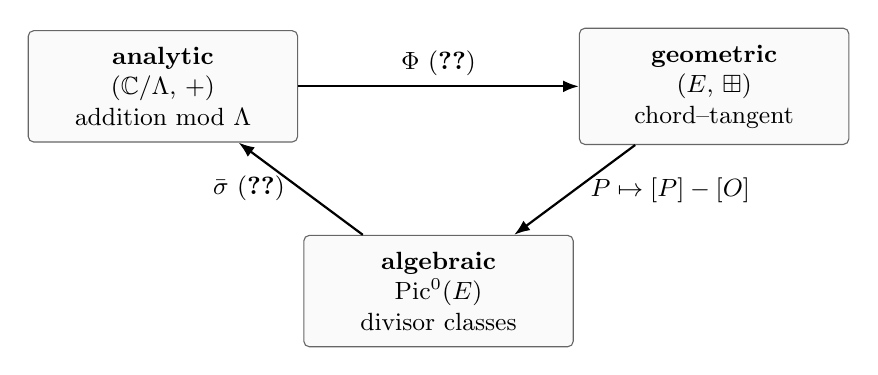
\begin{tikzpicture}[every node/.style={font=\small}]
  \node[visualnode, text width=3.0cm] (an) at (0,0)
    {\textbf{analytic}\\$(\C/\Lambda,\,+)$\\addition mod $\Lambda$};
  \node[visualnode, text width=3.0cm] (geo) at (7,0)
    {\textbf{geometric}\\$(E,\,\boxplus)$\\chord--tangent};
  \node[visualnode, text width=3.0cm] (alg) at (3.5,-2.6)
    {\textbf{algebraic}\\$\Pic^0(E)$\\divisor classes};
  \draw[arrow] (an) -- node[above, labelnode] {$\Phi$ (\cref{thm:emb-iso})} (geo);
  \draw[arrow] (geo) -- node[right, labelnode, xshift=2pt] {$P \mapsto [P]-[O]$} (alg);
  \draw[arrow] (alg) -- node[left, labelnode, xshift=-2pt] {$\bar\sigma$ (\cref{thm:div-pic-iso})} (an);
\end{tikzpicture}
\caption{Three views of one group. The Weierstrass embedding \(\Phi\) identifies
the analytic and geometric groups; the Abel--Jacobi map \(\bar\sigma\) identifies
the algebraic group \(\Pic^0(E)\) with the torus; and \(P \mapsto [P]-[O]\) closes
the triangle. All three are the same abelian group.}
\label{fig:syn-threeviews}
\end{figure}

\begin{keyidea}{Final takeaway}
The chord--tangent law is the visible projective shadow of the simple addition
law \([u]+[v]=[u+v]\) on the complex torus. The Weierstrass embedding turns
addition into line intersection because line intersections give principal
divisors, and principal divisors have zero Abel sum. The torus explains the
group; the cubic displays it; the divisor classes name it.
\end{keyidea}

\section{Further Directions}
\label{sec:syn-further}

Everything below takes \((E, O) \cong (\C/\Lambda, 0)\) as its starting point.

\subsection{The \texorpdfstring{$j$}{j}-Invariant and Moduli}
\label{sec:syn-j}

\Cref{prop:lat-normal-form} reduced the classification of complex tori to
\(\HH / \mathrm{SL}_2(\Z)\). A single number resolves it: the \emph{\(j\)-invariant}
\[
  j = 1728\,\frac{g_2^3}{g_2^3 - 27 g_3^2} = 1728\,\frac{g_2^3}{\Delta}.
\]
Two elliptic curves over \(\C\) are isomorphic iff they have the same \(j\), and
\(j : \HH / \mathrm{SL}_2(\Z) \to \C\) is a bijection: the moduli space of elliptic
curves is the \(j\)-line \(\C\). As a function of \(\tau\), \(j(\tau)\) is the
basic modular function, invariant under \(\mathrm{SL}_2(\Z)\). The lemniscatic
curve \(y^2 = 4x^3 - 4x\) of our examples has \(j = 1728\)
(\cref{ex:syn-j1728}), a curve with extra symmetry (complex multiplication by
\(\Z[i]\)).

\subsection{Isogenies and Torsion}
\label{sec:syn-isogeny}

An \emph{isogeny} is a nonconstant holomorphic group homomorphism
\(E \to E'\); analytically it is induced by \(z \mapsto \alpha z\) for some
\(\alpha \in \C\) with \(\alpha\Lambda \subseteq \Lambda'\). The most important
example is multiplication by \(n\),
\[
  [n] : E \to E, \qquad P \mapsto \underbrace{P \oplus \cdots \oplus P}_{n},
\]
a rational map of degree \(n^2\) whose kernel is the \(n\)-torsion. Over \(\C\),
\[
  E[n] = \{ P : nP = O \} = \tfrac1n\Lambda / \Lambda \cong (\Z/n\Z)^2 ,
\]
generalizing the \(E[2] \cong (\Z/2\Z)^2\) of \cref{sec:cases-torsion}. The
torsion carries the Weil pairing \(E[n] \times E[n] \to \mu_n\), a perfect
alternating pairing that pervades the arithmetic theory.

\subsection{Elliptic Curves over \texorpdfstring{$\Q$}{Q} and Finite Fields}
\label{sec:syn-arithmetic}

Because the group law is given by rational formulas (\cref{prop:coord-field}), it
runs over any field. Two cases drive modern number theory.

Over \(\Q\), the \emph{Mordell--Weil theorem} states that \(E(\Q)\) is a finitely
generated abelian group,
\[
  E(\Q) \cong \Z^r \oplus E(\Q)_{\mathrm{tors}},
\]
with \(r\) the \emph{rank}. The torsion is completely classified (Mazur); the rank
is deep, conjecturally governed by the \(L\)-function through the
Birch--Swinnerton-Dyer conjecture.

Over a finite field \(\F_p\), the group \(E(\F_p)\) is finite with
\[
  \#E(\F_p) = p + 1 - a_p, \qquad |a_p| \le 2\sqrt p
\]
(Hasse's bound). The difficulty of inverting the map \(n \mapsto nP\) in
\(E(\F_p)\) --- the elliptic curve discrete logarithm problem --- is the basis of
elliptic-curve cryptography.

\subsection{Modular Forms and Modularity}
\label{sec:syn-modular}

The Eisenstein series \(G_4, G_6\) that produced \(g_2, g_3\)
(\cref{def:wp-eisenstein}) are the first \emph{modular forms}: under
\(\Lambda \mapsto \alpha\Lambda\) they scale by \(\alpha^{-4}, \alpha^{-6}\), so as
functions of \(\tau\) they satisfy \(G_k(\tfrac{a\tau+b}{c\tau+d}) =
(c\tau+d)^k G_k(\tau)\). The discriminant \(\Delta = g_2^3 - 27g_3^2\) is a cusp
form of weight \(12\), and \(j = 1728 g_2^3/\Delta\) has weight \(0\)
(\cref{ex:syn-weight}). The arithmetic of elliptic curves over \(\Q\) is bound to
modular forms by the \emph{modularity theorem} (Wiles, Taylor--Wiles,
Breuil--Conrad--Diamond--Taylor): every elliptic curve over \(\Q\) arises from a
weight-two modular form. Its most famous consequence is Fermat's Last Theorem.

\subsection{Where to Read Next}
\label{sec:syn-reading}

Silverman's \emph{The Arithmetic of Elliptic Curves} \cite{silverman} is the
standard entry to the arithmetic theory; Silverman--Tate, \emph{Rational Points on
Elliptic Curves} \cite{silverman-tate}, is a gentler start. For the
complex-analytic and modular side, see Diamond--Shurman, \emph{A First Course in
Modular Forms} \cite{diamond-shurman}, and Serre, \emph{A Course in Arithmetic}
\cite{serre}. Each of these opens at the point reached here: the elliptic curve is
a complex torus, and its group law is addition.

\section{Summary}
\label{sec:syn-summary}

The chord--tangent law is addition on \(\C/\Lambda\) transported by
\((\wp, \wp')\), and the same group appears in three guises --- analytic,
geometric, algebraic (\cref{fig:syn-threeviews}). From this single fact the
subject branches: the \(j\)-invariant classifies the curves
(\cref{sec:syn-j}); isogenies and torsion organize the maps between them
(\cref{sec:syn-isogeny}); the rational group law carries the theory over \(\Q\)
and \(\F_p\) into number theory and cryptography (\cref{sec:syn-arithmetic}); and
the Eisenstein series tie it to modular forms and, through modularity, to Fermat
(\cref{sec:syn-modular}). The torus was the key throughout: it makes a mysterious
geometric construction into the most natural thing in the world, the addition of
points.

\section*{Exercises}
\addcontentsline{toc}{section}{Exercises}

\begin{exercise}
\label{ex:syn-j1728}
Compute the \(j\)-invariant of \(E : y^2 = 4x^3 - 4x\) (so \(g_2 = 4\),
\(g_3 = 0\)). Confirm \(\Delta = 64\) and \(j = 1728\). What is \(j\) for a curve
with \(g_2 = 0\) (so \(y^2 = 4x^3 - g_3\))?
\end{exercise}

\begin{exercise}
\label{ex:syn-torsion}
Show that over \(\C\), \(E[n] = \tfrac1n\Lambda/\Lambda \cong (\Z/n\Z)^2\), and
that multiplication by \(n\), realized as \(z \mapsto nz\) on \(\C/\Lambda\), is an
\(n^2\)-to-one map, so \([n]\) has degree \(n^2\).
\end{exercise}

\begin{exercise}
\label{ex:syn-weight}
Using \(G_k(\alpha\Lambda) = \alpha^{-k} G_k(\Lambda)\), show that under
\(\Lambda \mapsto \alpha\Lambda\) one has \(g_2 \mapsto \alpha^{-4} g_2\),
\(g_3 \mapsto \alpha^{-6} g_3\), \(\Delta \mapsto \alpha^{-12}\Delta\), and hence
\(j\) is invariant. Interpret these as the weights \(4, 6, 12, 0\).
\end{exercise}

\begin{exercise}
\label{ex:syn-hasse}
Take \(E : y^2 = x^3 + 1\) over \(\F_5\). List its affine points, add the point at
infinity, and find \(\#E(\F_5)\). Check that it satisfies the Hasse bound
\(|{\#E(\F_5)} - 6| \le 2\sqrt5\), and identify the group structure.
\end{exercise}


\appendix
\part{Appendices}
% Complex-Analysis Toolkit  (prerequisites refresher; reference appendix for the
% single-variable complex analysis the book relies on)
\chapter{Complex-Analysis Toolkit}
\label{app:A}

This appendix collects, for reference, the results from a first course in complex
analysis that the main text uses. Proofs are in any standard text --- Ahlfors
\cite{ahlfors}, Stein--Shakarchi \cite{stein-shakarchi}, Conway \cite{conway} ---
and we state the facts precisely and note where each is invoked.

\section{Holomorphic and Meromorphic Functions}
\label{sec:A-holo}

A function \(f\) on an open \(U \subseteq \C\) is \emph{holomorphic} if it is
complex-differentiable at every point; equivalently it is given near each point by
a convergent power series. It is \emph{meromorphic} on \(U\) if it is holomorphic
off a discrete set of poles. Near a point \(p\) a meromorphic \(f \not\equiv 0\)
has a \emph{Laurent expansion}
\[
  f(z) = \sum_{k \ge m} c_k (z-p)^k, \qquad c_m \ne 0,
\]
and the integer \(m = \ord_p(f)\) is the \emph{order}: \(m > 0\) a zero, \(m < 0\)
a pole of order \(-m\), \(m = 0\) a nonzero finite value. The \emph{residue} is the
coefficient \(\Res_p f = c_{-1}\). These notions are intrinsic to a Riemann surface
because they are unchanged by holomorphic coordinate changes
(\cref{rem:div-ord-welldef}), which is what lets us speak of orders and residues on
\(T = \C/\Lambda\) throughout \crefrange{ch:elliptic_liouville}{ch:divisors}.

\section{Liouville's Theorem and the Maximum Modulus Principle}
\label{sec:A-liouville}

\begin{theorem}[Liouville]
\label{thm:A-liouville}
A bounded entire function (holomorphic on all of \(\C\)) is constant.
\end{theorem}

\begin{theorem}[Maximum modulus]
\label{thm:A-maxmod}
A nonconstant holomorphic function on a connected open set has no interior local
maximum of \(|f|\). Consequently a holomorphic function on a compact connected
Riemann surface is constant.
\end{theorem}

These are the engine of \cref{thm:ell-const}: a holomorphic elliptic function is
bounded (by periodicity and compactness of the fundamental parallelogram), hence
constant. The same statements force \(L(0) = \C\) and \(\Omega(T) = \C\,dz\) in
\cref{ch:riemann_roch}.

\section{Residues and the Residue Theorem}
\label{sec:A-residues}

\begin{theorem}[Residue theorem in the plane]
\label{thm:A-residue-plane}
If \(f\) is meromorphic on a domain containing a positively oriented simple closed
curve \(\gamma\) and its interior, with no poles on \(\gamma\), then
\[
  \frac{1}{2\pi i} \oint_\gamma f(z)\,dz = \sum_{p \text{ inside}} \Res_p f .
\]
\end{theorem}

On a compact Riemann surface there is no boundary, and the global form is a
vanishing theorem.

\begin{theorem}[Sum of residues on a compact surface]
\label{thm:A-residue-compact}
For a meromorphic \(1\)-form \(\omega\) on a compact Riemann surface \(X\),
\(\sum_{p \in X} \Res_p \omega = 0\).
\end{theorem}

The planar version drives the period-parallelogram computations of
\cref{ch:elliptic_liouville} (the boundary integral vanishes because opposite
sides cancel, leaving \(\sum \Res = 0\)); the compact version is the clean
statement behind \(\deg\divisor(f) = 0\) applied to \(df/f\) in
\cref{thm:div-degzero}. Both are global Stokes-type statements
(\cref{app:B}).

\section{The Argument Principle and Winding Numbers}
\label{sec:A-argument}

\begin{theorem}[Argument principle]
\label{thm:A-argument}
If \(f\) is meromorphic inside and on a positively oriented simple closed curve
\(\gamma\), with no zeros or poles on \(\gamma\), then
\[
  \frac{1}{2\pi i} \oint_\gamma \frac{f'(z)}{f(z)}\,dz = Z - P,
\]
the number of zeros minus the number of poles inside, with multiplicity. The
left side is the winding number of \(f \circ \gamma\) about \(0\).
\end{theorem}

Applied on a period parallelogram, this gives the valence theorem
\cref{thm:ell-valence} (\#zeros \(=\) \#poles for an elliptic function) and,
through \(\oint z\,f'/f\), the Abel relation \cref{thm:ell-abel}; the integrality
of the winding number is the \(2\pi i\,\Z\) in those proofs
(\cref{ex:ell-winding}).

\section{Pointers}
\label{sec:A-pointers}

The Weierstrass \(M\)-test (uniform convergence of a series dominated by a
convergent series of constants) justifies the convergence of the \(\wp\)-series in
\cref{prop:wp-converges}. The implicit function theorem provides holomorphic charts
on a smooth plane curve, making \(E\) a Riemann surface in \cref{sec:emb-l3o}. A
nonconstant holomorphic map between compact Riemann surfaces is a finite branched
cover and is surjective; this underlies the degree-two cover \(\wp : T \to \CP^1\)
(\cref{sec:wp-roots}) and the surjectivity of \(\Phi\) in \cref{thm:emb-iso}.

% The Exam-to-Lecture Bridge  (source §2, relocated; records how the material
% grew out of a course's midterm and final, with cross-references to the chapters)
\chapter{The Exam-to-Lecture Bridge}
\label{app:B}

These notes grew out of a course whose midterm and final assembled exactly the
tools the main argument needs. This appendix records that lineage, for readers who
want to see where each ingredient came from; each item points to the chapter that
develops it in full.

\section{From the Midterm}
\label{sec:B-midterm}

\begin{enumerate}
\item \textbf{Differential forms and Stokes' theorem.} Integral theorems are best
read as statements about differential forms. The residue theorem on a compact
Riemann surface (\cref{thm:A-residue-compact}) is another global Stokes-type
identity --- the vanishing of a sum of local data --- and it is the form used in
\cref{ch:divisors}.

\item \textbf{Cauchy--Green and residues.} That residues are global obstructions
--- local singular data constrained by a global sum --- is the philosophy behind
Abel's law (\cref{ch:elliptic_liouville,ch:abel}): the zeros and poles of an
elliptic function cannot be prescribed freely.

\item \textbf{The torus as a quotient.} The midterm computed invariants of real
and complex tori. The complex torus \(T = \C/\Lambda\) is the source of the group
law here (\cref{ch:lattices,ch:torus_group_surface}).

\item \textbf{Euler characteristic of a torus.} The midterm found \(\chi(T) = 0\);
with \(\chi = 2 - 2g\) this gives genus \(g = 1\) (\cref{prop:tg-euler}), exactly
the genus that makes Riemann--Roch take its elliptic-curve form.
\end{enumerate}

\section{From the Final}
\label{sec:B-final}

\begin{enumerate}
\item \textbf{Compact Riemann surfaces and meromorphic maps.} The final used that
nonconstant holomorphic maps between compact Riemann surfaces are finite branched
coverings. Here \(\wp, \wp'\) are meromorphic on the compact surface \(T\), and
\(\wp : T \to \CP^1\) is the degree-two cover of \cref{sec:wp-roots}.

\item \textbf{Principal divisors have degree zero.} Proved on the final via the
logarithmic derivative \(df/f\); it is the degree half of Abel's law
(\cref{thm:div-degzero}).

\item \textbf{Riemann--Roch.} On a genus-one surface it predicts the dimensions
\(\ell(nO) = n\) that force \(1, \wp, \wp'\) to be the coordinate functions ---
counts the present treatment derives elementarily
(\cref{prop:rr-counts,sec:rr-functions}).

\item \textbf{The torus and \(\wp\).} The final's \(\wp\)-problem derived
\(\wp'^2 = 4\wp^3 - g_2\wp - g_3\) (\cref{thm:wp-ode}), which is precisely the
equation of the plane cubic.
\end{enumerate}

\begin{keyidea}{Exam-to-lecture bridge}
The midterm supplies the geometric and differential-form intuition; the final
supplies the compact Riemann surface tools. Together they explain why the
algebraic-looking chord--tangent rule is forced by complex analysis: the torus has
genus one, principal divisors balance, and Riemann--Roch produces \(\wp\) and
\(\wp'\).
\end{keyidea}

% The Sage-to-TikZ Figure Pipeline  (documents the sagemath/ pipeline so every
% figure in the book is reproducible)
\chapter{The Sage-to-TikZ Figure Pipeline}
\label{app:C}

Every figure in this book is drawn with exact coordinates, not freehand. The
geometry --- lattice points, the torus and sphere silhouettes, the elliptic curve
samples, the chord and tangent intersections --- is computed by a set of SageMath
scripts that emit \LaTeX{} macros, which the TikZ figures then reference. This
appendix documents the pipeline so the figures can be regenerated and checked.

\section{Overview}
\label{sec:C-overview}

The pipeline lives in the \texttt{sagemath/} directory (a sibling of
\texttt{book/}). Each script \texttt{NN\_name.sage} computes coordinates and
writes them to \texttt{coords\_name.tex} as \verb|\newcommand| definitions; the
driver \texttt{build\_coords.sh} runs all scripts and concatenates their output
into a single \texttt{coords.tex}. The document \verb|\input|s that file, so a
figure can write, e.g., \verb|\fill (\chordPx,\chordPy)| and get the precise
Sage-computed point.

\section{The Scripts}
\label{sec:C-scripts}

\begin{center}
\footnotesize
\begin{tabular}{@{}lll@{}}
\hline
Script & Output \texttt{coords\_*} & Role\\
\hline
\texttt{01\_lattice}          & \texttt{lattice}        & lattice basis and cell data\\
\texttt{02\_torus\_group\_law}& \texttt{group}          & group-law points $u,v,u{+}v$\\
\texttt{03\_elliptic\_curve}  & \texttt{curve}          & the roots $e_1,e_2,e_3$\\
\texttt{04\_chord\_tangent}   & \texttt{chord}          & chord example $P,Q,R,-R$\\
\texttt{05\_tangent\_double}  & \texttt{tangent}        & doubling example $P,R,2P$\\
\texttt{06\_two\_torsion}     & \texttt{torsion}        & two-torsion + vertical-line points\\
\texttt{07\_branched\_cover}  & \texttt{branch}         & branched-cover data\\
\texttt{08\_torus\_render}    & \texttt{torus}          & torus arcs (precise torus)\\
\texttt{09\_torus\_markers}   & \texttt{torus\_markers} & markers on the torus\\
\texttt{10\_sphere\_render}   & \texttt{sphere}         & sphere arcs (the $\CP^1$ image)\\
\texttt{11\_correspondence}   & \texttt{correspondence} & three-panel markers\\
\texttt{12\_curve\_sample}    & \texttt{curve\_sample}  & arcs of $y^2=4x^3-4x$\\
\hline
\end{tabular}
\end{center}

\noindent The macros are named after their script: e.g.\ \texttt{01\_lattice}
emits \verb|\latwax|, \verb|\latomegaone|; \texttt{04\_chord\_tangent} emits
\verb|\chordPx|, \verb|\chordQx|, \verb|\chordRx|, \verb|\chordSx|;
\texttt{11\_correspondence} emits the \verb|\cor...| family; and the three
\verb|\drawprecise...| macros consume \texttt{coords\_torus}, \texttt{coords\_sphere},
and \texttt{coords\_curve\_sample}.

The running example throughout is \(E : y^2 = 4x^3 - 4x\) (\(g_2 = 4\), \(g_3 = 0\),
roots \(-1, 0, 1\)), with a fixed lattice whose basis is recorded in
\texttt{coords\_lattice.tex}.

\section{The Convenience Macros}
\label{sec:C-macros}

Three painting macros, defined in \texttt{book/preamble.tex}, encapsulate the most
intricate figures so a chapter can drop them into a scope:
\begin{itemize}
\item \verb|\drawprecisetorus| --- the tilted torus (outer/inner silhouettes,
  meridians, latitudes split into visible/hidden arcs), from \texttt{coords\_torus};
\item \verb|\drawprecisesphere| --- the \(\CP^1\) sphere matching the torus style,
  from \texttt{coords\_sphere};
\item \verb|\drawprecisecurve| --- the real locus of \(y^2 = 4x^3 - 4x\) (compact
  oval plus unbounded branch, with the three branch points), from
  \texttt{coords\_curve\_sample}.
\end{itemize}

\section{Building and Consuming the Coordinates}
\label{sec:C-build}

The driver \texttt{sagemath/build\_coords.sh} runs every \texttt{0?\_*.sage} in
order and concatenates the per-script files into \texttt{coords.tex}. The book's
preamble loads
\begin{quote}\ttfamily
\textbackslash input\{\textbackslash sagedir/coords.tex\}\\
\textbackslash input\{\textbackslash sagedir/coords\_torus.tex\}\\
\textbackslash input\{\textbackslash sagedir/coords\_curve\_sample.tex\}
\end{quote}
where \verb|\sagedir| points at \texttt{../sagemath}. The aggregated
\texttt{coords.tex} contains the lattice, group, curve, chord, tangent, torsion,
branch, torus-marker, sphere, correspondence, and curve-sample macros; the precise
torus rendering \texttt{coords\_torus.tex} is generated by
\texttt{08\_torus\_render} but loaded separately.

\section{Regenerating the Figures}
\label{sec:C-regen}

With SageMath installed, regenerate all coordinates and rebuild the book by
\begin{quote}\ttfamily
cd sagemath \&\& ./build\_coords.sh\\
cd ../book \&\& pdflatex main.tex \&\& pdflatex main.tex
\end{quote}
The committed \texttt{coords*.tex} files let the book compile \emph{without} Sage;
they need to be regenerated only if a \texttt{.sage} script changes (for instance to
use a different lattice or curve). If a new figure needs precise geometry, add a
script \texttt{sagemath/NN\_name.sage} that writes \texttt{coords\_name.tex}, list
that file in \texttt{build\_coords.sh}, and \verb|\input| it (or rely on the
aggregated \texttt{coords.tex}). Coordinates should never be hand-typed: keeping
them under Sage control is what makes the figures exact and the book reproducible.

% Solutions to Exercises  (full solutions, all chapters)
% Add one \section per chapter as chapters are written. Reference each exercise
% with \cref{ex:...} so numbering stays automatic.
\chapter{Solutions to Exercises}
\label{app:D}

This appendix gives full solutions to every exercise. Solutions are grouped by
chapter and reference each exercise by its number.

\section{Chapter 1}
\label{sec:soln-ch1}

\paragraph{\Cref{ex:intro-thirdpoint}.}
Write the line and the cubic in homogeneous coordinates on \(\CP^2\).
Substituting the linear equation of the line into the cubic gives a single
homogeneous cubic equation in one projective parameter along the line, i.e.\ a
degree-three form. Over \(\C\), and counting multiplicity, such a form has
exactly three roots, so the line meets the cubic in three points counted with
multiplicity. Two of them are \(P\) and \(Q\); the third is \(R\). Passing to
the projective plane is what guarantees the count is exact --- it supplies the
points at infinity where, for example, a vertical line meets the curve. The
precise statement is B\'ezout's theorem (\cref{ch:lines_divisors}).

\paragraph{\Cref{ex:intro-tangent}.}
As \(Q \to P\) along the curve, the secant line through \(P\) and \(Q\)
approaches the tangent line at \(P\). The chord construction needs two
intersection points to start from; when the two points coincide, ``meeting the
curve at \(P\) twice'' is exactly the condition that the line be tangent there,
i.e.\ that it meet \(E\) at \(P\) with intersection multiplicity at least two.
So doubling \(P \oplus P\) uses the tangent at \(P\), whose third intersection
with \(E\) is then reflected. Intersection multiplicity is made precise in
\cref{ch:lines_divisors}, and the tangent (doubling) law in
\cref{ch:chord_tangent_cases}.

\paragraph{\Cref{ex:intro-liouville}.}
A holomorphic function on \(\C/\Lambda\) lifts to a holomorphic function on
\(\C\) that is periodic with respect to \(\Lambda\); its values are determined
by those on the (compact) fundamental parallelogram, so it is bounded, hence by
Liouville's theorem constant. Therefore the only holomorphic functions on
\(\C/\Lambda\) are the constants (\cref{ch:elliptic_liouville}).

\paragraph{\Cref{ex:intro-map-arrows}.}
Reading the arrows of \cref{fig:dependency}:
\begin{itemize}
\item \(T \xrightarrow{\ \Phi\ } (\wp,\wp')\): the Weierstrass functions are
  built on the torus in \cref{ch:weierstrass_wp}.
\item \((\wp,\wp') \to E\): the differential equation embeds the torus as the
  cubic, \cref{ch:weierstrass_wp,ch:embedding}.
\item \(E \to (\text{a line cuts } P+Q+R)\): intersecting \(E\) with a line,
  \cref{ch:lines_divisors}.
\item \((\text{line}) \to (\text{principal divisors have Abel sum zero})\):
  a line gives a principal divisor, \cref{ch:lines_divisors}.
\item \((\text{Abel sum zero}) \to T\) with label \(P+Q+R=O\): Abel's sum law,
  \cref{ch:abel}, transported in \cref{ch:transport}.
\end{itemize}

\section{Chapter 2}
\label{sec:soln-ch2}

\paragraph{\Cref{ex:lat-area}.}
Writing \(\omega_1 = x_1 + iy_1\) and \(\omega_2 = x_2 + iy_2\), the
parallelogram spanned by the vectors \((x_1,y_1)\) and \((x_2,y_2)\) has area
\(|x_1 y_2 - x_2 y_1|\). A short computation gives
\(\operatorname{Im}(\overline{\omega_1}\,\omega_2)
= x_1 y_2 - y_1 x_2\), so the area is
\(|\operatorname{Im}(\overline{\omega_1}\,\omega_2)|\), which is nonzero exactly
because \(\omega_1,\omega_2\) are \(\R\)-independent. Under a change of basis by
\(M \in \mathrm{GL}_2(\Z)\) (\cref{prop:lat-basis-change}) the area scales by
\(|\det M| = 1\), so it is a lattice invariant, the \emph{covolume} of
\(\Lambda\).

\paragraph{\Cref{ex:lat-discrete}.}
The function \((s,t) \mapsto |s\omega_1 + t\omega_2|\) is continuous and, by
\(\R\)-independence, strictly positive on the compact set
\(K = \{(s,t) \in \R^2 : \max(|s|,|t|) = 1\}\); let \(c > 0\) be its minimum.
For integers \(a,b\) not both zero, put \(n = \max(|a|,|b|) \ge 1\); then
\((a/n, b/n) \in K\), so \(|a\omega_1 + b\omega_2| = n\,|(a/n)\omega_1 +
(b/n)\omega_2| \ge cn = c\,\max(|a|,|b|)\). In particular
\(m(\Lambda) \ge c > 0\). A bounded region \(\{|\lambda| \le R\}\) then forces
\(\max(|a|,|b|) \le R/c\), leaving finitely many \((a,b)\), so finitely many
lattice points.

\paragraph{\Cref{ex:lat-square}.}
For \(\Lambda = \Z + \Z i\), the matrix
\(M = \left(\begin{smallmatrix} 0 & -1 \\ 1 & 0 \end{smallmatrix}\right)
\in \mathrm{SL}_2(\Z)\) sends \(\tau = i\) to
\(\frac{0\cdot i - 1}{1 \cdot i + 0} = -1/i = i\), so it fixes \(i\). It
corresponds to the basis change \((\omega_1,\omega_2) = (1,i) \mapsto
(\omega_1', \omega_2') = (i, -1) = (i\cdot 1,\, i\cdot i)\), i.e.\ multiplication
of the lattice by \(i\): the order-four rotational symmetry of the square
lattice. (Its square \(-I\) acts trivially on \(\tau\), reflecting that \(-1\)
also preserves \(\Lambda\).)

\paragraph{\Cref{ex:lat-homothety-iso}.}
If \(z \sim w\) in \(\C/\Lambda\), i.e.\ \(z - w \in \Lambda\), then
\(\alpha z - \alpha w \in \alpha\Lambda = \Lambda'\), so
\([z] \mapsto [\alpha z]\) is well defined; the inverse is
\([w] \mapsto [\alpha^{-1} w]\), so it is a bijection, and it is continuous both
ways because \(\pi' \circ (\alpha \cdot) = (\text{map}) \circ \pi\) with
\(z \mapsto \alpha z\) continuous. In the charts of
\cref{thm:lat-riemann-surface} the map lifts to \(z \mapsto \alpha z\), which is
holomorphic with holomorphic inverse; hence it is biholomorphic.

\paragraph{\Cref{ex:lat-chart-radius}.}
Take \(\Lambda = \Z + \Z i\), so \(m(\Lambda) = 1\) and \(m(\Lambda)/2 = 1/2\).
For any \(r > 1/2\) the open disk \(D(0, r)\) contains both \(-1/2\) and
\(1/2\), and these differ by \(1 \in \Lambda\); hence
\(\pi(-1/2) = \pi(1/2)\) while \(-1/2 \ne 1/2\), so \(\pi\) is not injective on
\(D(0,r)\). Conversely, for \(r \le 1/2\) any two points \(z, z' \in D(z_0, r)\)
satisfy \(|z - z'| < 2r \le 1 = m(\Lambda)\); a nonzero lattice vector has length
at least \(m(\Lambda)\), so \(z - z' \in \Lambda\) forces \(z = z'\) and \(\pi\)
is injective. Thus injectivity holds exactly up to radius \(m(\Lambda)/2\), and
the threshold is sharp. (The proof's choice \(r < m(\Lambda)/2\) is a convenient
strict bound; any \(r \le m(\Lambda)/2\) would serve.)

\section{Chapter 3}
\label{sec:soln-ch3}

\paragraph{\Cref{ex:tg-lie-holo}.}
Cover \(T \times T\) by products \(U_{z_0} \times U_{w_0}\) of the charts
\(\varphi_{z_0}, \varphi_{w_0}\) from \cref{thm:lat-riemann-surface}. In the
source product chart the points are \((z, w)\) with \(z \in D(z_0, r)\),
\(w \in D(w_0, r)\), and \(m([z],[w]) = [z+w]\); reading the target through the
chart \(\varphi_{z_0 + w_0}\) (valid near \([z_0+w_0]\)) the map is
\((z, w) \mapsto z + w\), a holomorphic function of two complex variables. Since
\(\pi\) is a local biholomorphism, \(m\) is holomorphic. For \(\iota\), the
local expression through \(\varphi_{z_0}\) and \(\varphi_{-z_0}\) is
\(z \mapsto -z\), holomorphic with holomorphic inverse \(z \mapsto -z\); hence
\(\iota\) is biholomorphic.

\paragraph{\Cref{ex:tg-two-torsion}.}
A point \([z]\) is fixed by \(\iota\) iff \([-z] = [z]\), i.e.\ \(2z \in
\Lambda\), i.e.\ \(z \in \tfrac12\Lambda\). Modulo \(\Lambda\), the quotient
\(\tfrac12\Lambda / \Lambda \cong (\tfrac12\Z/\Z)^2 \cong (\Z/2\Z)^2\) has
exactly four elements, represented by
\(0,\ \tfrac{\omega_1}{2},\ \tfrac{\omega_2}{2},\ \tfrac{\omega_1+\omega_2}{2}\).
These are precisely the solutions of \(2[z] = [0]\), the two-torsion subgroup
\(T[2] \cong (\Z/2\Z)^2\).

\paragraph{\Cref{ex:tg-first-iso}.}
The map \(e : \R \to S^1\), \(t \mapsto e^{2\pi i t}\), satisfies
\(e(t_1 + t_2) = e(t_1)e(t_2)\), so it is a homomorphism; it is continuous and
surjective (every unit-modulus number is \(e^{2\pi i t}\) for some \(t\)), and
\(e(t) = 1 \iff t \in \Z\), so \(\ker e = \Z\). The first isomorphism theorem
gives a continuous group isomorphism \(\bar e : \R/\Z \to S^1\). Finally
\(\R/\Z\) is the continuous image of the compact interval \([0,1]\), hence
compact, and \(S^1\) is Hausdorff, so the continuous bijection \(\bar e\) is a
homeomorphism.

\paragraph{\Cref{ex:tg-euler-refine}.}
Cut \(P_\Lambda\) along a diagonal into two triangles before gluing. After
identification one finds, for example, \(V = 1\) (all corners still collapse to
one vertex), \(E = 3\) (the two boundary loops \(a, b\) plus the diagonal
\(d\)), and \(F = 2\) (the two triangles). Then
\(\chi = V - E + F = 1 - 3 + 2 = 0\), the same value: the Euler characteristic
is independent of the chosen CW structure.

\paragraph{\Cref{ex:tg-homeo-not-biholo}.}
Both lattices are of the form \(\Z + \Z\tau\) with \(\tau = i\) and
\(\tau = 2i\), so by \cref{cor:tg-abelian} each torus is homeomorphic (and
diffeomorphic) to \(S^1 \times S^1\); composing the two homeomorphisms gives a
homeomorphism between them. For the complex structure, \cref{prop:lat-normal-form}
says \(\C/(\Z+\Z i)\) and \(\C/(\Z+\Z\,2i)\) are biholomorphic iff \(i\) and
\(2i\) are related by an element of \(\mathrm{SL}_2(\Z)\). Granting that both lie
in the closed fundamental domain and are not identified there, they are
inequivalent, so the tori are not biholomorphic. There is no contradiction with
\cref{cor:tg-abelian}: that corollary asserts only a \emph{topological}
isomorphism, and \cref{warn:tg-not-biholo} stresses that the homeomorphism
\(\Psi\) is not holomorphic. Homeomorphic surfaces can carry inequivalent complex
structures.

\section{Chapter 4}
\label{sec:soln-ch4}

\paragraph{\Cref{ex:ell-field}.}
For \(f, g\) elliptic, each of \(f \pm g, fg, f/g\) is meromorphic, and
periodicity is pointwise: \((fg)(z+\lambda) = f(z+\lambda)g(z+\lambda) =
f(z)g(z)\), and similarly for the others; the constants \(0, 1\) are elliptic, so
we have a field. Differentiating \(f(z+\lambda) = f(z)\) gives
\(f'(z+\lambda) = f'(z)\), so \(f'\) is elliptic. For fixed \(a\), \((f(\cdot+a))
(z+\lambda) = f(z+a+\lambda) = f(z+a)\), so \(f(z+a)\) is elliptic. If
\(f(-z) = f(z)\), differentiate: \(-f'(-z) = f'(z)\), i.e.\ \(f'(-z) = -f'(z)\),
so \(f'\) is odd.

\paragraph{\Cref{ex:ell-no-order-one}.}
An order-one function would have, in a period parallelogram, a single simple
pole and no other poles; the residue there is nonzero (the defining feature of a
simple pole), contradicting \(\sum \Res = 0\) (\cref{thm:ell-residues}). Hence no
order-one elliptic function exists. For order two the total pole multiplicity is
\(2\): either two simple poles at \(p_1 \ne p_2\) with residues \(r_1, r_2\), and
\cref{thm:ell-residues} forces \(r_1 + r_2 = 0\); or a single pole of order two,
with Laurent expansion \(c_{-2}(z-p)^{-2} + c_{-1}(z-p)^{-1} + \cdots\) whose
residue is \(c_{-1}\), and since it is the only pole, \(\sum\Res = c_{-1} = 0\).

\paragraph{\Cref{ex:ell-double-pole-zeros}.}
By \cref{thm:ell-valence} the order-two function \(f\) has exactly two zeros
\(z_1, z_2\) (with multiplicity). Its only pole is the double pole at \([0]\), so
\cref{thm:ell-abel} reads \(z_1 + z_2 - (0 + 0) \in \Lambda\), i.e.\
\(z_2 \equiv -z_1 =: -w\). The zeros are \([w], [-w]\). Now \(f - f(z_0)\) is
again elliptic of order two with the same double pole at \([0]\); one zero is
\(z_0\), so by the same argument its second zero is \(-z_0\). Thus \(f\) takes
each value at a pair \(\pm z_0\), which is the hallmark of an even function
\(f(-z) = f(z)\).

\paragraph{\Cref{ex:ell-sum-values}.}
The function \(f - c_1\) is elliptic of order \(N\) with the same poles
\(p_1, \dots, p_N\) as \(f\) and with zeros the solutions \(z_1^{(1)}, \dots\) of
\(f = c_1\). By \cref{thm:ell-abel}, \(\sum_k z_k^{(1)} - \sum_k p_k \in
\Lambda\). The same for \(c_2\): \(\sum_k z_k^{(2)} - \sum_k p_k \in \Lambda\).
Subtracting the two congruences, the pole sums cancel and
\(\sum_k z_k^{(1)} \equiv \sum_k z_k^{(2)} \pmod \Lambda\). Hence the sum of the
solution set of \(f = c\) is, modulo \(\Lambda\), independent of \(c\); its common
value (equal to \(\sum p_k\) mod \(\Lambda\)) is an invariant of \(f\).

\paragraph{\Cref{ex:ell-winding}.}
Let \(\gamma(s) = a + s\omega_1\), \(s \in [0,1]\), avoid the zeros and poles of
\(f\). Then \(\int_a^{a+\omega_1} (f'/f)\,dz = \int_0^1 \frac{d}{ds}\log f(\gamma(s))\,ds
= \log f(a+\omega_1) - \log f(a)\) for a continuous branch of \(\log f\) along
\(\gamma\). The real part is \(\log|f(a+\omega_1)| - \log|f(a)| = 0\) because
\(f(a+\omega_1) = f(a)\); the imaginary part is the net change of argument,
\(2\pi k_1\), where \(k_1 \in \Z\) is the number of times the image curve
\(s \mapsto f(\gamma(s))\) winds around \(0\). Hence the integral equals
\(2\pi i\,k_1\), and \(k_1\) is precisely that winding number.

\section{Chapter 5}
\label{sec:soln-ch5}

\paragraph{\Cref{ex:div-hom}.}
By \cref{prop:div-prin-subgroup}, \(\divisor(fg) = \divisor(f) + \divisor(g)\),
so \(\divisor\) is a homomorphism from \((\mathcal{M}(X)^\times, \cdot)\) to
\((\Div(X), +)\). If \(\divisor(f) = 0\) then \(f\) has no zeros or poles, so it
is holomorphic and nonvanishing on the compact \(X\); by \cref{thm:ell-const}
(or the maximum modulus principle) \(f\) is a nonzero constant. Conversely
\(\divisor(c) = 0\). Hence \(\ker\divisor = \C^\times\).

\paragraph{\Cref{ex:div-ord-welldef}.}
Independence of coordinate is \cref{rem:div-ord-welldef}: a coordinate change
\(t = s\,h(s)\), \(h(0)\ne0\), turns \(f = t^m u\) into
\(f = s^m\,(h^m\, u\!\circ\! t)\) with a nonvanishing unit, so the exponent
\(m\) is unchanged. For the sum, write \(f = t^{a}u\), \(g = t^{b}v\) with
\(a = \ord_p f \le b = \ord_p g\) and units \(u, v\). Then
\(f + g = t^{a}(u + t^{b-a}v)\); the factor \(u + t^{b-a}v\) is holomorphic, so
\(\ord_p(f+g) \ge a = \min(a,b)\), and if \(a < b\) it equals \(u(0) \ne 0\) at
\(t=0\), giving \(\ord_p(f+g) = a\).

\paragraph{\Cref{ex:div-pic-split}.}
The map \(D \mapsto (\degdiv D,\ D - (\degdiv D)[0])\) is a homomorphism, since
\(\degdiv\) is and the second slot is linear in \(D\); its second component has
degree \(\degdiv D - \degdiv D = 0\), so it lands in \(\Z \oplus \Div^0(T)\). The
inverse is \((n, E) \mapsto E + n[0]\), so it is an isomorphism. Principal
divisors have degree \(0\) and lie in the \(\Div^0\) slot, so quotienting gives
\(\Pic(T) \cong \Z \oplus \Pic^0(T)\); with \(\Pic^0(T) \cong T\) from
\cref{thm:div-pic-iso}, \(\Pic(T) \cong \Z \oplus T\).

\paragraph{\Cref{ex:div-distinct-points}.}
If \([a] = [b]\) then \([a] - [b] = 0 = \divisor(1)\) is principal. Conversely, if
\([a] - [b] = \divisor(f)\) is principal, then it lies in \(\Div^0(T)\) and
\cref{thm:ell-abel} (via \cref{prop:div-sigma-kills-prin}) gives
\(\smap([a]-[b]) = [a] - [b] = 0\) in \(T\), i.e.\ \([a] = [b]\). On \(\CP^1\)
the function \((z-a)/(z-b)\) has divisor \([a] - [b]\) for any \(a \ne b\), so the
statement fails there. The torus version recovers \cref{cor:ell-order2}: a
principal divisor \([a] - [b]\) with \(a \ne b\) would be the divisor of an
order-one elliptic function (one simple zero, one simple pole), which does not
exist.

\paragraph{\Cref{ex:div-sigma-compute}.}
The divisor \(D = [\tfrac12] + [\tfrac{\tau}{2}] + [\tfrac{1+\tau}{2}] - 3[0]\)
has \(\degdiv D = 3 - 3 = 0\). Its Abel sum is
\[
  \smap(D) = \Bigl[\tfrac12 + \tfrac{\tau}{2} + \tfrac{1+\tau}{2}\Bigr]
  = \Bigl[\tfrac{2 + 2\tau}{2}\Bigr] = [\,1 + \tau\,] = [0],
\]
since \(1 + \tau \in \Lambda\). So \(D\) has degree zero and Abel sum zero, hence
is a candidate for a principal divisor --- and indeed it is: the three nonzero
half-periods \(\tfrac12, \tfrac{\tau}{2}, \tfrac{1+\tau}{2}\) are exactly the
two-torsion points of \cref{ex:tg-two-torsion}, and \(D = \divisor(\wp')\), the
divisor of the Weierstrass derivative (simple zeros at the half-periods, a
triple pole at \([0]\)), as we will see in \cref{ch:weierstrass_wp}.

\section{Chapter 6}
\label{sec:soln-ch6}

\paragraph{\Cref{ex:rr-point-lemma}.}
Let \(D = \sum n_q\,q\). An \(f \in L(D+p)\) may have a pole at \(p\) of order up
to \(n_p + 1\). In a coordinate \(t\) at \(p\), the map
\(\lambda : L(D+p) \to \C\) sending \(f\) to its Laurent coefficient of order
\(-(n_p+1)\) (the most negative now allowed) is linear. Its kernel is exactly the
functions whose pole order at \(p\) is at most \(n_p\), i.e.\ \(L(D)\). Hence
\(L(D+p)/L(D) \hookrightarrow \C\), so \(\ell(D+p) - \ell(D) = \dim\operatorname{im}\lambda
\in \{0,1\}\).

\paragraph{\Cref{ex:rr-neg-degree}.}
If \(\deg D < 0\) and \(0 \ne f \in L(D)\), then \(\divisor(f) \ge -D\) has
degree \(0\) (\cref{thm:div-degzero}) but \(\deg(-D) > 0\), impossible; so
\(L(D) = 0\). For the inequality, induct on \(\deg D\) downward using the point
lemma: any \(D\) can be written \(D = D_0 + \sum_{j=1}^{k} p_j\) with
\(\deg D_0 \le 0\) and \(k = \deg D - \deg D_0\); since
\(\ell(D_0) \le 1\) (it is \(0\) for negative degree, and for degree \(0\) a
nonzero \(f \in L(D_0)\) has \(\divisor(f) = -D_0\), so \(D_0 \sim 0\) and
\(\ell(D_0) = 1\)) and each added point raises \(\ell\) by at most
one (\cref{ex:rr-point-lemma}), \(\ell(D) \le 1 + (\deg D - \deg D_0) \le \deg D + 1\).

\paragraph{\Cref{ex:rr-degree-one-unique}.}
A divisor of degree one is \(\sum n_q\,q\) with \(\sum n_q = 1\); it is effective
(\(\ge 0\)) iff all \(n_q \ge 0\), which with sum \(1\) means exactly one
coefficient equals \(1\) and the rest \(0\), i.e.\ a single point. By
\cref{prop:rr-counts}, \(\ell([a]) = 1\), so \(L([a]) = \C\) (constants); the
effective divisors linearly equivalent to \([a]\) are the \(\divisor(f) + [a]\)
for \(0 \ne f \in L([a])\), i.e.\ \(f\) constant, giving only \([a]\) itself.

\paragraph{\Cref{ex:rr-canonical-deg}.}
By \cref{prop:rr-canonical}, \(K \sim 0\), so \(\ell(K) = \ell(0) = 1 = g\). Taking
\(D = K\) in Riemann--Roch: \(\ell(K) - \ell(K - K) = \deg K + 1 - g\), i.e.\
\(\ell(K) - \ell(0) = \deg K + 1 - g\). With \(\ell(K) = \ell(0) = 1\) and
\(g = 1\) this reads \(0 = \deg K + 1 - 1\), so \(\deg K = 0 = 2g - 2\),
consistent.

\paragraph{\Cref{ex:rr-cubic-count}.}
The pole orders at \(O\) are
\[
  1 \!:\! 0,\quad \wp \!:\! 2,\quad \wp^2 \!:\! 4,\quad \wp^3 \!:\! 6,\quad
  \wp' \!:\! 3,\quad \wp\wp' \!:\! 5,\quad \wp'^2 \!:\! 6,
\]
all \(\le 6\) and with no other poles, so all seven lie in \(L(6O)\). Since
\(\ell(6O) = 6 < 7\), they are linearly dependent: \(\sum c_i\,F_i = 0\)
nontrivially. The only two functions with a pole of order exactly \(6\) are
\(\wp^3\) and \(\wp'^2\); their leading Laurent coefficients at \(O\) are the
only order-\(6\) contributions, so for the order-\(6\) pole to cancel, the
coefficients of \(\wp^3\) and \(\wp'^2\) must be nonzero and balance. If either
were zero, the other would contribute an uncancelled order-six pole, contradicting
\(\sum c_i F_i = 0\) (a holomorphic, indeed zero, function). Hence both appear,
and solving for the relation gives \(\wp'^2 = 4\wp^3 - g_2\wp - g_3\).

\section{Chapter 7}
\label{sec:soln-ch7}

\paragraph{\Cref{ex:wp-convergence}.}
Lattice points are uniformly separated (\cref{ex:lat-discrete}), so disjoint disks
of radius \(\rho = \tfrac12 m(\Lambda)\) about them are contained in the disk of
radius \(R + \rho\) once \(|\lambda| \le R\); comparing areas bounds their number
by \((R+\rho)^2/\rho^2 = O(R^2)\). Splitting into annuli \(n \le |\lambda| < n+1\)
(each with \(O(n)\) points) gives \(\sum_\lambda |\lambda|^{-s} \le \sum_n O(n)\,
n^{-s} = \sum_n O(n^{1-s}) < \infty\) for \(s > 2\). The differentiated terms
\(\frac{d}{dz}\bigl((z-\lambda)^{-2} - \lambda^{-2}\bigr) = -2(z-\lambda)^{-3}\)
satisfy \(|{-2}(z-\lambda)^{-3}| \le 16/|\lambda|^3\) for \(|z| \le R\),
\(|\lambda| \ge 2R\), which is summable (\(s = 3\)); uniform convergence of the
differentiated series justifies term-by-term differentiation, and adding the
\(\lambda = 0\) term \(\tfrac{d}{dz}z^{-2} = -2z^{-3}\) gives
\(\wp'(z) = -2\sum_{\lambda \in \Lambda}(z-\lambda)^{-3}\).

\paragraph{\Cref{ex:wp-g2g3}.}
From \cref{prop:wp-laurent}, \(\wp = z^{-2} + 3G_4 z^2 + 5G_6 z^4 + O(z^6)\), so
\(a_2 = 3G_4\), \(a_4 = 5G_6\). Using \(\wp' = -2z^{-3} + 2a_2 z + 4a_4 z^3 +
\cdots\), one computes \(\wp'^2 - 4\wp^3 = -20a_2 z^{-2} - 28 a_4 + O(z^2)\).
Choosing \(g_2 = 20 a_2\) and \(g_3 = 28 a_4\) cancels the \(z^{-2}\) term and the
constant; substituting \(a_2 = 3G_4\), \(a_4 = 5G_6\) gives \(g_2 = 60G_4\),
\(g_3 = 140 G_6\).

\paragraph{\Cref{ex:wp-roots-distinct}.}
The cubic \(4x^3 - g_2 x - g_3 = 4\bigl(x^3 - \tfrac{g_2}{4}x - \tfrac{g_3}{4}\bigr)\)
is monic after dividing by \(4\), with \(p = -g_2/4\), \(q = -g_3/4\). The
discriminant of a monic cubic \(x^3 + px + q\) is \(\prod_{i<j}(e_i-e_j)^2 =
-4p^3 - 27q^2\). Hence
\[
  \prod_{i<j}(e_i-e_j)^2 = -4\Bigl(-\tfrac{g_2}{4}\Bigr)^3 - 27\Bigl(-\tfrac{g_3}{4}\Bigr)^2
  = \frac{g_2^3}{16} - \frac{27 g_3^2}{16} = \frac{g_2^3 - 27g_3^2}{16},
\]
so \(\Delta = g_2^3 - 27g_3^2 = 16\prod_{i<j}(e_i-e_j)^2\). By
\cref{prop:wp-roots}(3) the \(e_i\) are distinct, so \(\Delta \ne 0\).

\paragraph{\Cref{ex:wp-field}.}
Write \(f = f_+ + f_-\) with \(f_\pm(z) = \tfrac12(f(z) \pm f(-z))\), both
elliptic, \(f_+\) even and \(f_-\) odd. By the generation step of
\cref{thm:wp-generation}, even elliptic functions lie in \(\C(\wp)\), so
\(f_+ = A(\wp)\) for a rational \(A\). Since \(\wp'\) is odd, \(f_-/\wp'\) is even,
hence \(f_-/\wp' = B(\wp)\) for a rational \(B\); thus \(f_- = B(\wp)\,\wp'\) and
\(f = A(\wp) + B(\wp)\,\wp'\). The fact \(\wp' \notin \C(\wp)\) guarantees this
representation is genuine and unique: if
\(A_1(\wp) + B_1(\wp)\wp' = A_2(\wp) + B_2(\wp)\wp'\) then
\((B_1 - B_2)(\wp)\,\wp' = (A_2 - A_1)(\wp) \in \C(\wp)\) forces
\(B_1 = B_2\) (else \(\wp' \in \C(\wp)\)) and then \(A_1 = A_2\).

\paragraph{\Cref{ex:wp-recurrence}.}
Differentiating \(\wp'^2 = 4\wp^3 - g_2\wp - g_3\) gives \(2\wp'\wp'' =
(12\wp^2 - g_2)\wp'\), and dividing by \(2\wp'\) (not identically zero),
\(\wp'' = 6\wp^2 - \tfrac12 g_2\). Write \(\wp = z^{-2} + \sum_{n\ge1} c_n z^{2n}\)
with \(c_n = (2n+1)G_{2n+2}\). Then \(\wp'' = 6z^{-4} + \sum_{n\ge1}
2n(2n-1)c_n z^{2n-2}\), while
\(6\wp^2 = 6z^{-4} + 12\sum_{n\ge1} c_n z^{2n-2} + 6\sum_{n\ge2}\bigl(\sum_{i+j=n}
c_i c_j\bigr)z^{2n-2}\). Matching the coefficient of \(z^{2n-2}\) for \(n \ge 3\)
(the cases \(n=1,2\) absorb \(g_2\)) gives \(2n(2n-1)c_n = 12c_n +
6\sum_{i+j=n}c_ic_j\), i.e.
\[
  c_n = \frac{3}{(2n+3)(n-2)}\sum_{\substack{i+j=n\\ i,j\ge1}} c_i c_j
  \qquad (n \ge 3).
\]
Since \(c_1 = 3G_4\) and \(c_2 = 5G_6\), this recurrence determines every
\(c_n\), hence every \(G_{2n+2}\), as a polynomial in \(G_4\) and \(G_6\); for
instance \(c_3 = \tfrac{3}{9\cdot1}c_1^2 = \tfrac13 c_1^2\), giving
\(G_8 = \tfrac{3}{7}G_4^2\).

\paragraph{\Cref{ex:wp-sigma-quasi}.}
Because \(\zeta' = -\wp\) is periodic, \(g(z) := \zeta(z+\omega_k) - \zeta(z)\) has
\(g' = 0\), so \(g \equiv \eta_k\) is constant; at \(z = -\omega_k/2\), oddness of
\(\zeta\) gives \(\eta_k = \zeta(\omega_k/2) - \zeta(-\omega_k/2) = 2\zeta(\omega_k/2)\).
Since \((\log\sigma)' = \sigma'/\sigma = \zeta\), the function
\(\log\frac{\sigma(z+\omega_k)}{\sigma(z)}\) has derivative
\(\zeta(z+\omega_k) - \zeta(z) = \eta_k\), so it equals \(\eta_k z + c_k\) for some
constant \(c_k\), i.e.\ \(\sigma(z+\omega_k) = \sigma(z)\,e^{\eta_k z + c_k}\).
Evaluate at \(z = -\omega_k/2\): the left side is \(\sigma(\omega_k/2)\), the right
\(\sigma(-\omega_k/2)e^{-\eta_k\omega_k/2 + c_k} = -\sigma(\omega_k/2)
e^{-\eta_k\omega_k/2 + c_k}\) (oddness), and \(\sigma(\omega_k/2) \neq 0\) since
\(\omega_k/2 \notin \Lambda\); hence \(e^{c_k - \eta_k\omega_k/2} = -1\) and
\(\sigma(z+\omega_k) = -\sigma(z)\,e^{\eta_k(z+\omega_k/2)}\).

\paragraph{\Cref{ex:wp-converse-check}.}
Using \(\sigma(z+\omega_k - c) = -\sigma(z-c)\,e^{\eta_k(z - c + \omega_k/2)}\) for
each shift \(c \in \{a_i, b_i\}\),
\[
  \frac{F(z+\omega_k)}{F(z)}
  = \frac{\prod_{i=1}^n\bigl(-e^{\eta_k(z - a_i + \omega_k/2)}\bigr)}
         {\prod_{i=1}^n\bigl(-e^{\eta_k(z - b_i + \omega_k/2)}\bigr)} .
\]
The numerator is \((-1)^n e^{\eta_k(nz - \sum a_i + n\omega_k/2)}\) and the
denominator \((-1)^n e^{\eta_k(nz - \sum b_i + n\omega_k/2)}\); the factor
\((-1)^n\) cancels because the two products have the \emph{same number} of factors
(degree zero), and the \(nz\) and \(n\omega_k/2\) terms cancel, leaving
\(\exp\!\bigl(\eta_k(\sum b_i - \sum a_i)\bigr)\). This is \(1\) because
\(\sum a_i = \sum b_i\) (Abel sum zero). Thus degree zero is used to cancel
\((-1)^n\) and the \(z\)-dependence, and Abel sum zero to kill the residual
exponent. For \([a] - [0]\) with \(a \notin \Lambda\) the counts match (degree
zero), so the candidate \(\sigma(z-a)/\sigma(z-0)\) has the right zeros and poles,
but \(\sum a_i - \sum b_i = a \notin \Lambda\), so \(F(z+\omega_k)/F(z) =
e^{\eta_k a} \neq 1\) in general: \(F\) is not elliptic, consistent with there
being no order-one elliptic function (\cref{cor:ell-order2}).

\section{Chapter 8}
\label{sec:soln-ch8}

\paragraph{\Cref{ex:emb-holo-origin}.}
Near \([0]\), the homogeneous representative \((z^3\wp, z^3\wp', z^3)\) has middle
entry tending to \(-2 \ne 0\), so divide by it: in the chart \(Y = 1\) the map is
\(z \mapsto (X, Z) = (\wp/\wp',\, 1/\wp')\). From \(\wp = z^{-2} + O(z^2)\),
\(\wp' = -2z^{-3} + O(z)\): \(\wp/\wp' = \frac{z^{-2} + \cdots}{-2z^{-3} + \cdots}
= -\tfrac12 z + O(z^3)\) and \(1/\wp' = -\tfrac12 z^3 + O(z^5)\). Both are
holomorphic at \(z = 0\) with value \((0,0) = O\), and \(X = \wp/\wp'\) has
derivative \(-\tfrac12 \ne 0\) there, so it is a local holomorphic coordinate and
\(\Phi\) is an immersion at \(O\) (indeed \(z\) and \(X\) agree to first order up
to the factor \(-\tfrac12\)).

\paragraph{\Cref{ex:emb-flex}.}
Write the curve as \(G = Y^2 Z - 4X^3 + g_2 X Z^2 + g_3 Z^3 = 0\). At
\(O = [0:1:0]\), \(\nabla G = (-12X^2 + g_2 Z^2,\ 2YZ,\ Y^2 + 2g_2 XZ + 3g_3 Z^2)
= (0, 0, 1) \ne 0\), so \(O\) is smooth with tangent \(Z = 0\). Substituting
\(Z = 0\) into \(G\) gives \(-4X^3 = 0\), a triple root, so \(Z = 0\) meets \(E\)
at \(O\) with multiplicity three; \(O\) is a flex. Hence the line \(Z = 0\) cuts
the divisor \(3O\) on \(E\), so \(3O = \divisor(\text{line}/\text{line})\) is
principal --- concretely \(3O \sim 3O\), and any two lines cut linearly equivalent
divisors, making \(3O\) the class that will be the group identity.

\paragraph{\Cref{ex:emb-fiber-lemma}.}
\Cref{lem:emb-fibers} is proved in the text: \(\wp - \wp(w)\) has order two, with
zeros \(w, -w\), so \(\wp(z) = \wp(w) \Rightarrow z \equiv \pm w\). Thus the fibers
of \(\wp : T \to \CP^1\) are the orbits \(\{z, -z\}\) of \(z \mapsto -z\), giving a
bijection \(T/\{\pm1\} \to \CP^1\). The fixed points of \(z \mapsto -z\) are the
four two-torsion points (\cref{ex:tg-two-torsion}); there the two sheets come
together, so they map to the branch values, namely \(\wp(\omega_i/2) = e_i\) and
\(\wp(0) = \infty\).

\paragraph{\Cref{ex:emb-two-torsion-image}.}
At \(z = 0\), \(\Phi(0) = O\). At a half-period \(\omega_i/2\), \(\wp'(\omega_i/2)
= 0\) (\cref{prop:wp-roots}) and \(\wp(\omega_i/2) = e_i\), so
\(\Phi(\omega_i/2) = (e_i, 0)\). The points of \(E\) fixed by \((x,y) \mapsto
(x,-y)\) satisfy \(y = -y\), i.e.\ \(y = 0\) (the three \((e_i, 0)\)) or the point
at infinity \(O\); these are exactly the four images, matching the two-torsion.

\paragraph{\Cref{ex:emb-involution}.}
The map \(\iota_E(x,y) = (x,-y)\) preserves \(y^2 = 4x^3 - g_2 x - g_3\) (the
right side depends only on \(x\)), fixes \(O\), and satisfies \(\iota_E^2 = \id\),
so it is a holomorphic involution. Its invariant function is \(x = \wp\), and two
points share an \(x\)-value iff they are \(\pm\)-related, so the quotient
\(E/\iota_E\) is the \(x\)-line \(\CP^1\). Under \(\Phi\), \(\iota_E\) pulls back to
the map with \(\wp(z) \mapsto \wp(z)\), \(\wp'(z) \mapsto -\wp'(z) = \wp'(-z)\),
i.e.\ \(z \mapsto -z\). Since the double cover \(\wp : T \to \CP^1\) has deck group
\(\{\pm1\}\) of order two, its unique nontrivial deck transformation is
\(z \mapsto -z\), which is \(\iota_E\).

\section{Chapter 9}
\label{sec:soln-ch9}

\paragraph{\Cref{ex:abel-independence}.}
Take \(D_1 = [a] - [0]\) with \(a \notin \Lambda\): \(\deg D_1 = 0\) but
\(\smap(D_1) = [a] \ne 0\), so \(D_1\) is not principal (a principal divisor of
this shape would be an order-one elliptic function, excluded by
\cref{cor:ell-order2}). Take \(D_2 = 2[0]\): \(\smap(D_2) = 2[0] = 0\) but
\(\deg D_2 = 2 \ne 0\), so \(D_2\) is not principal. Thus each condition can hold
while the other fails, so neither alone characterizes principality.

\paragraph{\Cref{ex:abel-three-point}.}
\Cref{cor:abel-three-point} is immediate from \cref{thm:abel-law}:
\([p]+[q]+[r]-3[0]\) has degree \(0\), and its Abel sum is \([p]+[q]+[r]\), zero
iff \(p+q+r \in \Lambda\). For existence/uniqueness of \(R\): given \(P = [p]\),
\(Q = [q]\), the equation \(P + Q + R = O\) in the group \(T\) has the unique
solution \(R = -(P+Q) = [-(p+q)]\). Through the isomorphism \(\Phi\) this \(R\) is
a well-defined point of the cubic, the reflection of the third intersection.

\paragraph{\Cref{ex:abel-period-integral}.}
Label the sides of \(P_a\) as in \cref{sec:ell-contour}. Pairing side
\(\mathrm{I}\) with \(\mathrm{III}\) (translates by \(\omega_2\), reversed) and
using \(\omega_2\)-periodicity of \(F'/F\),
\(\int_{\mathrm{I}} + \int_{\mathrm{III}} = -\omega_2 \int_{a}^{a+\omega_1}
(F'/F)\,dz\); pairing \(\mathrm{II}\) with \(\mathrm{IV}\) gives
\(+\omega_1 \int_{a}^{a+\omega_2}(F'/F)\,dz\). Each remaining integral is the
change of a branch of \(\log F\) along a side; since \(F(a+\omega_k) = F(a)\), the
real part returns to its start and the imaginary part changes by \(2\pi\) times an
integer (the winding number, \cref{ex:ell-winding}), so each integral lies in
\(2\pi i\,\Z\). Hence \(\oint z(F'/F)\,dz = \omega_1\cdot 2\pi i\,k_2 - \omega_2
\cdot 2\pi i\,k_1 \in 2\pi i\,\Lambda\).

\paragraph{\Cref{ex:abel-addition-function}.}
The divisor \(D = [a] + [b] - [a+b] - [0]\) has \(\deg D = 2 - 2 = 0\) and Abel
sum \(\smap(D) = [a] + [b] - [a+b] - [0] = (a + b) - (a+b) = 0\) in \(T\). By
sufficiency in \cref{thm:abel-law}, \(D\) is principal, so some elliptic \(F\) has
\(\divisor(F) = D\); its zeros \(a, b\) and poles \(a+b, 0\) encode the
group sum \(a + b\). By contrast \([a] - [0]\) with \(a \ne 0\) has Abel sum
\([a] \ne 0\), so it is \emph{not} principal --- there is no elliptic function with
a single simple zero and a single simple pole, consistent with
\cref{cor:ell-order2}.

\paragraph{\Cref{ex:abel-kernel}.}
Both \(\deg\) and \(\smap\) are homomorphisms \(\Div(T) \to \Z\) and
\(\Div(T) \to T\), so \((\deg, \smap)\) is a homomorphism to \(\Z \oplus T\). It
is surjective: \((n, [a]) = (\deg, \smap)\bigl(n[0] + ([a] - [0])\bigr)\), since
that divisor has degree \(n\) and Abel sum \([a]\). Its kernel is the divisors
with \(\deg = 0\) and \(\smap = 0\), which by \cref{thm:abel-law} are exactly
\(\Prin(T)\). The first isomorphism theorem then gives \(\Div(T)/\Prin(T) =
\Pic(T) \cong \Z \oplus T\), matching \cref{ex:div-pic-split}.

\section{Chapter 10}
\label{sec:soln-ch10}

\paragraph{\Cref{ex:lin-vertical}.}
The vertical line \(x = c\) is \(X - cZ = 0\). On \(E\), \(y^2 = 4c^3 - g_2 c - g_3
=: y_0^2\), giving the two affine points \((c, \pm y_0)\); and the line passes
through \(O = [0:1:0]\) (it contains the direction \([0:1:0]\), since
\(X - cZ\) vanishes there). So \(L \cdot E = (c, y_0) + (c, -y_0) + O\), which has
degree three as required. By \cref{thm:lin-collinear} these three sum to \(O\):
\((c, y_0) \oplus (c, -y_0) \oplus O = O\), i.e.\ \((c, y_0) \oplus (c, -y_0) = O\).
Thus \((c, -y_0) = -(c, y_0)\), the reflection across the \(x\)-axis of
\cref{sec:emb-reflection}.

\paragraph{\Cref{ex:lin-mult-welldef}.}
If \(m, m'\) both satisfy \(m(P), m'(P) \ne 0\), then \(m/m'\) is a rational
function on \(E\) with neither zero nor pole at \(P\), hence
\(\ord_P(m/m') = 0\). Therefore \(\ord_P(\ell/m) = \ord_P(\ell/m') +
\ord_P(m'/m) = \ord_P(\ell/m')\), so the multiplicity does not depend on the
auxiliary form.

\paragraph{\Cref{ex:lin-tangent}.}
By definition \(I_P(L,E) = \ord_P(\ell/m)\ge 1\) exactly when \(P \in L\). Choose a
local coordinate \(t\) on \(E\) at \(P\) and parametrize \(E\) by \(\gamma(t)\) with
\(\gamma(0) = P\). Then \(I_P(L,E) \ge 2\) iff \((\ell/m)(\gamma(t))\) vanishes to
order \(\ge 2\), iff \(\frac{d}{dt}(\ell/m)(\gamma(t))|_0 = 0\), iff the line
\(\ell = 0\) contains the tangent direction \(\gamma'(0)\) --- i.e.\ \(L\) is the
tangent line to \(E\) at \(P\). When \(L\) is tangent, \(I_P(L,E) \ge 2\) absorbs
two of the three intersections (\cref{prop:lin-bezout}), leaving one further point
\(R'\) (possibly \(= P\) at a flex), so \(L \cdot E = 2P + R'\).

\paragraph{\Cref{ex:lin-infinity-mult}.}
With \(v = 4u^3 - g_2 u v^2 - g_3 v^3\) and \(v = O(u^3)\) near \(0\): substituting
the ansatz \(v = c_3 u^3 + c_5 u^5 + \cdots\) (only odd powers by the symmetry
\(u \mapsto -u\), \(v \mapsto -v\)), the terms \(g_2 u v^2\) and \(g_3 v^3\) are
\(O(u^7)\), so to leading order \(v = 4u^3 + O(u^5)\); hence \(c_3 = 4\) and
\(\ord_O(Z/Y) = \ord_O v = 3\). Since \(Y\) is a unit at \(O\), \(\ord_O(Z|_E) =
3\) and \(\divisor_0(Z|_E) = 3O\).

\paragraph{\Cref{ex:lin-three-collinear}.}
Let \(R\) be the third intersection of the line through \(P\) and \(Q\) with \(E\),
so \(L \cdot E = P + Q + R\). By \cref{thm:lin-collinear},
\(P \oplus Q \oplus R = O\), hence \(R = -(P \oplus Q)\) and
\(P \oplus Q = -R\), the reflection of \(R\). When \(P = Q\) the chord degenerates;
the correct line is the \emph{tangent} to \(E\) at \(P\), which meets \(E\) at
\(2P + R\) (\cref{ex:lin-tangent}), giving \(2P = -R\) --- the doubling rule.

\section{Chapter 11}
\label{sec:soln-ch11}

\paragraph{\Cref{ex:tr-unique-transport}.}
If \(\boxdot\) makes \(\Phi\) a homomorphism, then \(\Phi(u+v) = \Phi(u) \boxdot
\Phi(v)\); since \(\Phi\) is a bijection, every \(P = \Phi(u)\), \(Q = \Phi(v)\),
and \(P \boxdot Q = \Phi(u+v)\) is determined --- this is \(\oplus\). It is abelian
because \(u + v = v + u\) in \(\C\); \(P \oplus O = \Phi(u + 0) = \Phi(u) = P\);
and \(\Phi(u) \oplus \Phi(-u) = \Phi(0) = O\), so \(\ominus\Phi(u) = \Phi(-u)\).

\paragraph{\Cref{ex:tr-identity-case}.}
The line \(L = PO\) through \(P = (x,y)\) and \(O = [0:1:0]\) is the vertical line
\(x = x_P\) (the point at infinity \(O\) lies on every vertical line). It meets
\(E\) at \((x, y)\), \((x, -y) = \ominus P\), and \(O\); so \(L \cdot E = P +
\ominus P + O\). By \cref{thm:lin-collinear}, \(P \oplus \ominus P \oplus O = O\),
which is automatic, and reading the chord--tangent recipe: the third point of
\(PO\) is \(\ominus P\), and \(P \oplus O = \ominus(\ominus P) = P\). Hence \(O\) is
the identity.

\paragraph{\Cref{ex:tr-associativity-free}.}
By \cref{thm:tr-main}, \(\boxplus = \oplus\), and \(\oplus\) is associative because
\(\Phi\) carries it to addition on \(\C/\Lambda\), which is associative since
addition in \(\C\) is: \((P \oplus Q) \oplus S = \Phi((u+v)+w) = \Phi(u+(v+w)) =
P \oplus (Q \oplus S)\). It reduces precisely to associativity of \(+\) in \(\C\).
The direct geometric proof is hard because associativity of the chord--tangent rule
is a nonobvious incidence statement about nine points and lines (the
Cayley--Bacharach/\(9\)-point theorem); the torus makes it a triviality by
linearizing the group.

\paragraph{\Cref{ex:tr-intrinsic}.}
By \cref{prop:tr-intrinsic} the operation \(\boxplus\) is defined using only lines
and \(O\) on \(E\), so it is one and the same regardless of how \(E\) was
presented. \Cref{thm:tr-main} applied to \(\Phi\) gives \(\oplus = \boxplus\), and
applied to \(\Phi'\) gives \(\oplus' = \boxplus\); hence \(\oplus = \oplus'\). Since
both \(\Phi\) and \(\Phi'\) are isomorphisms onto the same \((E, \boxplus)\), the
composite \(\Phi^{-1}\!\circ \Phi'\) is a group isomorphism
\(\C/\Lambda' \to \C/\Lambda\), forcing \(\Lambda\) and \(\Lambda'\) to be
homothetic (\cref{prop:lat-normal-form}): the same cubic comes only from
homothetic lattices.

\paragraph{\Cref{ex:tr-translation}.}
Under \(\Phi\), the translation \(P \mapsto P \oplus A\) corresponds to
\(z \mapsto z + a\) on \(T\), where \(a = \Phi^{-1}(A)\); this is the biholomorphism
\(\tau_a\) of \cref{prop:tg-lie}. Conjugating by \(\Phi\),
\(P \mapsto P \oplus A = \Phi(\Phi^{-1}(P) + a)\) is a composition of
biholomorphisms, hence a biholomorphism of \(E\). The addition map \(E \times E \to
E\) and inversion are holomorphic (transported from \(T\)), so \(E\) is a complex
Lie group acting on itself by holomorphic translations.

\section{Chapter 12}
\label{sec:soln-ch12}

\paragraph{\Cref{ex:cases-chord-vieta}.}
Substituting \(y = mx + k\) into \(y^2 = 4x^3 - g_2 x - g_3\) gives
\(4x^3 - m^2 x^2 - (g_2 + 2mk)x - (g_3 + k^2) = 0\), a cubic whose three roots are
\(x_P, x_Q, x_R\). By Vieta's formula the sum of the roots is the negative of the
\(x^2\)-coefficient over the leading coefficient: \(x_P + x_Q + x_R = m^2/4\),
hence \(x_R = \tfrac{m^2}{4} - x_P - x_Q\). The third intersection is
\(R = (x_R, m x_R + k)\), and \(P \oplus Q = -R = (x_R, -(m x_R + k))\).

\paragraph{\Cref{ex:cases-tangent-slope}.}
Differentiating \(y^2 = 4x^3 - g_2 x - g_3\) implicitly: \(2y\,y' = 12x^2 - g_2\),
so the tangent slope at \(P = (x_P, y_P)\) is \(m = (12 x_P^2 - g_2)/(2 y_P)\). The
tangent meets \(E\) at \(P\) with multiplicity two, so in the cubic of the previous
exercise \(x_P\) is a double root and \(x_P + x_P + x_{2P} = m^2/4\), giving
\(x_{2P} = \tfrac{m^2}{4} - 2x_P\). If \(y_P = 0\), the slope \(m\) is infinite:
the tangent is vertical, meeting \(E\) at \(P\) (doubly) and \(O\), so
\(R = O\) and \(2P = \ominus O = O\), matching that \(P\) is two-torsion.

\paragraph{\Cref{ex:cases-two-torsion-sum}.}
The line \(y = 0\) (the \(x\)-axis) meets \(E : y^2 = 4x^3 - g_2 x - g_3\) where
\(4x^3 - g_2 x - g_3 = 0\), i.e.\ at \((e_1,0), (e_2,0), (e_3,0) = T_1, T_2, T_3\);
these are exactly the nonzero two-torsion points. As three points on a line,
\cref{thm:lin-collinear} gives \(T_1 \oplus T_2 \oplus T_3 = O\). In
\(E[2] \cong (\Z/2\Z)^2\) the three nonzero elements are \(T_1, T_2, T_3\), and
indeed the sum of all nonzero elements of \((\Z/2\Z)^2\) is \((1,1)+(1,0)+(0,1) =
(0,0)\), consistent.

\paragraph{\Cref{ex:cases-flex-three-torsion}.}
If \(3P = O\), then in the divisor language \(3[P] - 3[O]\) is principal, so by
\cref{thm:lin-collinear} (with \(P = Q = R\)) the line \(L\) with \(L \cdot E = 3P\)
exists --- the tangent at \(P\) meets \(E\) only at \(P\), with multiplicity three,
which is the definition of an inflection point. Conversely a flex \(P\) has
\(L \cdot E = 3P\), so \(3P \oplus = O\), i.e.\ \(3P = O\). The point \(O\) is a
flex by \cref{prop:emb-flex} (the line at infinity meets \(E\) at \(O\) with
multiplicity three), consistent with \(3O = O\).

\section{Chapter 13}
\label{sec:soln-ch13}

\paragraph{\Cref{ex:coord-yform}.}
With \(b = y_1 - m x_1\), \(-(m x_3 + b) = -m x_3 - (y_1 - m x_1) = m(x_1 - x_3)
- y_1\). The second form is preferable numerically because it uses the input point
\((x_1, y_1)\) directly and avoids forming the intercept \(b\) as a separate
quantity (one fewer subtraction, less cancellation error); it also makes the
geometric reading clear --- start at \(P\), move by slope \(m\) over the run
\(x_1 - x_3\), then the sign records the reflection.

\paragraph{\Cref{ex:coord-commute}.}
The slope \(m = (y_2-y_1)/(x_2-x_1) = (y_1-y_2)/(x_1-x_2)\) is unchanged by
swapping \(P \leftrightarrow Q\). Then \(x_3 = m^2/4 - x_1 - x_2\) is symmetric in
\(x_1, x_2\). For \(y_3\), note the line intercept \(b = y_1 - m x_1 = y_2 - m x_2\)
is the same computed from either point (both lie on the line), so
\(y_3 = -(m x_3 + b)\) is manifestly symmetric. Hence \(P \oplus Q = Q \oplus P\).

\paragraph{\Cref{ex:coord-limit}.}
On \(E\), \(y_2^2 - y_1^2 = 4(x_2^3 - x_1^3) - g_2(x_2 - x_1)\). Factoring,
\((y_2-y_1)(y_2+y_1) = (x_2-x_1)\bigl(4(x_2^2 + x_2 x_1 + x_1^2) - g_2\bigr)\), so
for \(x_2 \ne x_1\),
\[
  m = \frac{y_2 - y_1}{x_2 - x_1} = \frac{4(x_2^2 + x_2 x_1 + x_1^2) - g_2}{y_2 + y_1}.
\]
As \(Q \to P\) (so \(x_2 \to x_1\), \(y_2 \to y_1 \ne 0\)) this tends to
\((4 \cdot 3x_1^2 - g_2)/(2y_1) = (12x_1^2 - g_2)/(2y_1)\), the tangent slope.
Correspondingly Vieta's \(x_1 + x_2 + x_R = m^2/4\) becomes \(2x_1 + x_R = m^2/4\),
so the addition formula limits to the doubling formula.

\paragraph{\Cref{ex:coord-vertical}.}
If \(x_1 = x_2\) then \(y_1^2 = y_2^2\) (both equal \(4x_1^3 - g_2 x_1 - g_3\)), so
\(y_2 = \pm y_1\); since \(P \ne Q\), \(y_2 = -y_1\), i.e.\ \(Q = \ominus P\). The
slope \((y_2-y_1)/(x_2-x_1)\) has zero denominator and is undefined --- the line is
vertical --- and the third intersection is \(O\), so \(P \oplus Q = \ominus O = O\).
Pseudocode:
\begin{quote}\ttfamily
add(P, Q):\\
\ \ if P = O: return Q;\quad if Q = O: return P\\
\ \ if x1 = x2:\\
\ \ \ \ if y1 = -y2: return O\quad // includes y1 = y2 = 0\\
\ \ \ \ else: return double(P)\quad // here P = Q, y1 != 0\\
\ \ else:\\
\ \ \ \ m = (y2-y1)/(x2-x1)\\
\ \ \ \ x3 = m\^{}2/4 - x1 - x2\\
\ \ \ \ return (x3, m*(x1-x3)-y1)
\end{quote}

\paragraph{\Cref{ex:coord-check}.}
With \(x_{2P} = \tfrac{25}{24}\) and \(y_{2P} = -\tfrac{35}{24\sqrt6}\):
\(y_{2P}^2 = \tfrac{1225}{576 \cdot 6} = \tfrac{1225}{3456}\), while
\(4x_{2P}^3 - 4x_{2P} = 4\cdot\tfrac{15625}{13824} - \tfrac{100}{24}
= \tfrac{62500}{13824} - \tfrac{57600}{13824} = \tfrac{4900}{13824} = \tfrac{1225}{3456}\).
They agree, so \(2P \in E\). Its inverse is the reflection
\(\ominus(2P) = \bigl(\tfrac{25}{24}, +\tfrac{35}{24\sqrt6}\bigr)\).

\section{Chapter 14}
\label{sec:soln-ch14}

\paragraph{\Cref{ex:aa-h-order}.}
\(h = \wp' - A\wp - B\) is a \(\C\)-linear combination of \(\wp', \wp, 1\), hence
elliptic. Its poles can only be at lattice points; at \(0\), \(\wp'\) has a pole
of order three and \(\wp\) of order two, so \(h\) has a pole of order exactly three
(the \(\wp'\) term dominates). Thus \(h\) has order three, and by
\cref{thm:ell-valence} exactly three zeros. By the choice of \(A, B\), \(h(u) =
\wp'(u) - A\wp(u) - B = 0\) and likewise \(h(v) = 0\), so \(u, v\) are zeros. The
case \(u \equiv \pm v\) is excluded because then \(\wp(u) = \wp(v)\) and the slope
\(A\) has a zero denominator (for \(u \equiv v\) one must instead take the limit,
giving the duplication formula; for \(u \equiv -v\) the sum \(u+v \equiv 0\) is a
pole of \(\wp\)).

\paragraph{\Cref{ex:aa-determinant-expand}.}
Expanding along the first column, the determinant equals
\[
  \bigl[\wp(v)(-\wp'(u{+}v)) - \wp(u{+}v)\wp'(v)\bigr]
  - \bigl[\wp(u)(-\wp'(u{+}v)) - \wp(u{+}v)\wp'(u)\bigr]
  + \bigl[\wp(u)\wp'(v) - \wp(v)\wp'(u)\bigr] = 0,
\]
a linear equation in the row \((1, \wp(u+v), -\wp'(u+v))\). Geometrically it says
\((\wp(u+v), -\wp'(u+v))\) lies on the line through \(P, Q\); its \(x\)-coordinate
is therefore the third root \(\tfrac{A^2}{4} - \wp(u) - \wp(v)\) of the
intersection cubic, which is \(\wp(u+v)\) --- exactly \cref{thm:aa-addition}.

\paragraph{\Cref{ex:aa-duplication-match}.}
Differentiating \(\wp'^2 = 4\wp^3 - g_2\wp - g_3\) gives \(2\wp'\wp'' = (12\wp^2 -
g_2)\wp'\), so \(\wp'' = 6\wp^2 - \tfrac12 g_2\). Hence
\[
  \frac{\wp''(u)}{\wp'(u)} = \frac{6\wp(u)^2 - \tfrac12 g_2}{\wp'(u)}
  = \frac{12\wp(u)^2 - g_2}{2\wp'(u)} = \frac{12x^2 - g_2}{2y},
\]
with \(x = \wp(u)\), \(y = \wp'(u)\) --- precisely the tangent slope of
\cref{thm:coord-double}. So the analytic duplication slope and the geometric
tangent slope agree.

\paragraph{\Cref{ex:aa-symmetry}.}
Swapping \(u \leftrightarrow v\) negates both \(\wp'(u) - \wp'(v)\) and
\(\wp(u) - \wp(v)\), leaving the slope \(A\) and hence \(A^2\) unchanged; the term
\(-\wp(u) - \wp(v)\) is symmetric, so \cref{thm:aa-addition} is symmetric. As
\(v \to 0\), \(\wp(v) \sim v^{-2} \to \infty\) and \(\wp'(v) \sim -2v^{-3}\), so
\(A \sim \wp'(v)/(-\wp(v)) \sim (-2v^{-3})/(-v^{-2}) = 2v^{-1}\) and
\(A^2/4 \sim v^{-2} \sim \wp(v)\); the divergent \(-\wp(v)\) and
\(+A^2/4\) cancel to leading order, leaving \(\wp(u+0) = \wp(u)\).

\paragraph{\Cref{ex:aa-three-term}.}
Replacing \(v\) by \(-v\) in \cref{thm:aa-addition} and using \(\wp(-v) = \wp(v)\),
\(\wp'(-v) = -\wp'(v)\),
\[
  \wp(u-v) = -\wp(u) - \wp(v) + \tfrac14\Bigl(\tfrac{\wp'(u) + \wp'(v)}{\wp(u) - \wp(v)}\Bigr)^2 .
\]
Adding to the formula for \(\wp(u+v)\), the two square terms combine via
\((a-b)^2 + (a+b)^2 = 2a^2 + 2b^2\) with \(a = \wp'(u)\), \(b = \wp'(v)\):
\[
  \wp(u+v) + \wp(u-v) = -2\wp(u) - 2\wp(v)
  + \frac{\wp'(u)^2 + \wp'(v)^2}{2(\wp(u) - \wp(v))^2}.
\]
By the differential equation \(\wp'(u)^2 = 4\wp(u)^3 - g_2\wp(u) - g_3\) (and
likewise for \(v\)), the numerator is a polynomial in \(\wp(u), \wp(v)\), so the
right-hand side is rational in \(\wp(u), \wp(v)\).

\section{Chapter 15}
\label{sec:soln-ch15}

\paragraph{\Cref{ex:wk-numeric-check}.}
\(\bigl(\tfrac{28\sqrt6}{125}\bigr)^2 = \tfrac{784 \cdot 6}{15625} =
\tfrac{4704}{15625}\). On the other side, with \(x_3 = -\tfrac{24}{25}\),
\(4x_3^3 - 4x_3 = 4\bigl(-\tfrac{13824}{15625}\bigr) + \tfrac{96}{25}
= -\tfrac{55296}{15625} + \tfrac{60000}{15625} = \tfrac{4704}{15625}\). They agree,
so \(P \oplus Q \in E\). Its inverse is \(\ominus(P\oplus Q) =
\bigl(-\tfrac{24}{25}, +\tfrac{28\sqrt6}{125}\bigr)\).

\paragraph{\Cref{ex:wk-doubling-symbolic}.}
The tangent at \(P\) has slope \(m = (12x_1^2 - g_2)/(2y_1)\) and intercept
\(b = y_1 - m x_1\). It meets \(E\) at \(P\) doubly, so \(x_1\) is a double root of
\(4x^3 - m^2 x^2 - (g_2 + 2mb)x - (g_3 + b^2) = 0\); matching against
\(4(x - x_1)^2(x - x_3)\), the \(x^2\)-coefficient gives \(2x_1 + x_3 = m^2/4\),
so \(x_3 = \tfrac{m^2}{4} - 2x_1\). Reflecting the third point,
\(2P = (x_3, -(m x_3 + b)) = \bigl(\tfrac{m^2}{4} - 2x_1,\, -m(\tfrac{m^2}{4} -
2x_1) - b\bigr)\), as in \cref{thm:coord-double}.

\paragraph{\Cref{ex:wk-standard-recompute}.}
By \cref{prop:wk-standard} with \(g_2 = 4\), \(g_3 = 0\): \(a = -1\), \(b = 0\), so
\(E' : Y^2 = X^3 - X\). In these coordinates \(P = (2, \sqrt6)\),
\(Q = (-\tfrac12, \tfrac{\sqrt6}{4})\) (halving the \(y\)'s), and the slope is
\(M = m/2 = \tfrac{3\sqrt6}{10}\), \(M^2 = \tfrac{54}{100}\). Then
\(X_3 = M^2 - X_1 - X_2 = \tfrac{27}{50} - \tfrac32 = -\tfrac{24}{25}\) (the same
\(x\)) and \(Y_3 = M(X_1 - X_3) - Y_1 = -\tfrac{14\sqrt6}{125}\). Mapping back by
\(y = 2Y\) gives \(y_3 = -\tfrac{28\sqrt6}{125}\), matching \cref{sec:wk-numeric}.

\paragraph{\Cref{ex:wk-pitfall-instances}.}
\emph{Pitfall 1.} Compute \(P \oplus (\ominus P)\) for \(P = (2, 2\sqrt6)\): the
line is the vertical \(x = 2\), which has \emph{no} third finite intersection. If
\(O\) is forgotten the sum looks undefined; including \(O\), the line meets \(E\)
at \(P, \ominus P, O\), so \(P \oplus (\ominus P) = O\).
\emph{Pitfall 2.} In \cref{sec:wk-numeric} the third intersection is
\(R = (-\tfrac{24}{25}, +\tfrac{28\sqrt6}{125})\); reporting \(R\) as \(P \oplus Q\)
gives the reflection of the true answer --- wrong by a sign in \(y\). The correct
sum is \(\ominus R = (-\tfrac{24}{25}, -\tfrac{28\sqrt6}{125})\).
\emph{Pitfall 7.} On the singular cubic \(y^2 = 4x^3\) (\(g_2 = g_3 = 0\),
\(\Delta = 0\)) the origin \((0,0)\) is a cusp; the tangent there is not defined and
the doubling formula divides by \(y = 0\). With \(\Delta \ne 0\)
(\cref{cor:wp-smooth}) no such point exists and every step is well defined.

\paragraph{\Cref{ex:wk-associativity-numeric}.}
Take \(S = (-1, 0)\), a two-torsion point. From \cref{sec:wk-numeric},
\(P \oplus Q = (-\tfrac{24}{25}, -\tfrac{28\sqrt6}{125})\). Computing with the
formulas (slope cases handled as in \cref{ex:coord-vertical}):
\[
  (P \oplus Q) \oplus S = (49, 280\sqrt6) = P \oplus (Q \oplus S),
\]
so the two bracketings agree, confirming associativity numerically (guaranteed by
\cref{rem:tr-associativity}). Both intermediate sums lie on \(E\), as a direct
substitution checks.

\section{Chapter 16}
\label{sec:soln-ch16}

\paragraph{\Cref{ex:syn-j1728}.}
With \(g_2 = 4\), \(g_3 = 0\): \(\Delta = g_2^3 - 27 g_3^2 = 64 - 0 = 64\), and
\[
  j = 1728\,\frac{g_2^3}{\Delta} = 1728\,\frac{64}{64} = 1728 .
\]
For a curve with \(g_2 = 0\) (and \(g_3 \ne 0\)), \(j = 1728 \cdot 0/\Delta = 0\):
these are the curves with \(j = 0\), having complex multiplication by
\(\Z[\zeta_3]\).

\paragraph{\Cref{ex:syn-torsion}.}
A point \([z]\) satisfies \(n[z] = [0]\) iff \(nz \in \Lambda\) iff
\(z \in \tfrac1n\Lambda\). Hence \(E[n] = \tfrac1n\Lambda/\Lambda\). The map
\(\tfrac1n\Lambda/\Lambda \to \Lambda/n\Lambda\), \(z \mapsto nz\), is an
isomorphism, and \(\Lambda \cong \Z^2\) gives \(\Lambda/n\Lambda \cong (\Z/n\Z)^2\).
The map \([n]: [z] \mapsto [nz]\) has fibers the cosets of \(E[n]\), of which there
are \(|E[n]| = n^2\); so \([n]\) is \(n^2\)-to-one and has degree \(n^2\).

\paragraph{\Cref{ex:syn-weight}.}
From \(G_k(\alpha\Lambda) = \sum_{\lambda\ne0}(\alpha\lambda)^{-k} =
\alpha^{-k} G_k(\Lambda)\): \(g_2 = 60 G_4 \mapsto \alpha^{-4} g_2\) and
\(g_3 = 140 G_6 \mapsto \alpha^{-6} g_3\). Then \(g_2^3 \mapsto \alpha^{-12} g_2^3\),
\(g_3^2 \mapsto \alpha^{-12} g_3^2\), so \(\Delta = g_2^3 - 27 g_3^2 \mapsto
\alpha^{-12}\Delta\). Finally \(j = 1728 g_2^3/\Delta \mapsto
1728\,\alpha^{-12}g_2^3 / (\alpha^{-12}\Delta) = j\): invariant. In modular-forms
language \(g_2, g_3, \Delta, j\) have weights \(4, 6, 12, 0\).

\paragraph{\Cref{ex:syn-hasse}.}
For \(E : y^2 = x^3 + 1\) over \(\F_5\), the squares are \(\{0,1,4\}\). Checking
each \(x\): \(x=0 \Rightarrow y^2 = 1\), \(y = \pm1\); \(x=1 \Rightarrow y^2 = 2\),
none; \(x=2 \Rightarrow y^2 = 9 = 4\), \(y = \pm2\); \(x=3 \Rightarrow y^2 = 28 =
3\), none; \(x=4 \Rightarrow y^2 = 65 = 0\), \(y = 0\). The affine points are
\((0,1), (0,4), (2,2), (2,3), (4,0)\) --- five of them --- plus \(O\), so
\(\#E(\F_5) = 6\). Then \(a_5 = 5 + 1 - 6 = 0\) and \(|a_5| = 0 \le 2\sqrt5 \approx
4.47\), satisfying Hasse. The point \((4,0)\) has order \(2\); a group of order \(6\)
with an element of order \(2\) is \(\Z/6\Z\), so \(E(\F_5) \cong \Z/6\Z\).


\backmatter

\addcontentsline{toc}{chapter}{Bibliography}
\begin{thebibliography}{9}

\bibitem{ahlfors}
L.~V. Ahlfors, \emph{Complex Analysis}, 3rd ed., McGraw--Hill, 1979.

\bibitem{stein-shakarchi}
E.~M. Stein and R.~Shakarchi, \emph{Complex Analysis}, Princeton Lectures in
Analysis II, Princeton University Press, 2003.

\bibitem{conway}
J.~B. Conway, \emph{Functions of One Complex Variable I}, 2nd ed., Graduate Texts
in Mathematics 11, Springer, 1978.

\bibitem{miranda}
R.~Miranda, \emph{Algebraic Curves and Riemann Surfaces}, Graduate Studies in
Mathematics 5, American Mathematical Society, 1995.

\bibitem{forster}
O.~Forster, \emph{Lectures on Riemann Surfaces}, Graduate Texts in Mathematics 81,
Springer, 1981.

\bibitem{silverman}
J.~H. Silverman, \emph{The Arithmetic of Elliptic Curves}, 2nd ed., Graduate Texts
in Mathematics 106, Springer, 2009.

\bibitem{silverman-tate}
J.~H. Silverman and J.~Tate, \emph{Rational Points on Elliptic Curves}, 2nd ed.,
Undergraduate Texts in Mathematics, Springer, 2015.

\bibitem{diamond-shurman}
F.~Diamond and J.~Shurman, \emph{A First Course in Modular Forms}, Graduate Texts
in Mathematics 228, Springer, 2005.

\bibitem{serre}
J.-P. Serre, \emph{A Course in Arithmetic}, Graduate Texts in Mathematics 7,
Springer, 1973.

\end{thebibliography}

\end{document}
